
\chapter{超出微扰论} \label{cha:29}


迄今为止所讨论的超对称应用大多数是用微扰论推导出来的. 在这一章, 我们将考虑一些即使把非微扰效应考虑在内也依旧成立的结果.

\section{超对称破缺的一般性质} \label{sec:29.1}

在已知粒子的谱中并没有观测到超对称, 所以它肯定破缺了. 我们在上一章看到, 超对称在标准模型的树级近似下破缺在实验上被排除了, %
并且电弱破缺标度与\,Planck\,或大统一标度之间的巨大差异指出超对称很可能是在某个跑动耦合常数变强时破缺的. %
因此对我们来说一件很重要的事是不借助微扰论来探索自发超对称破缺.

我们在\,\ref{sec:26.7}\,节看到, 作用量的超对称性表明存在守恒流$\,S^{\mu}(x)$. 从方程(\ref{26.A.2})的意义上说, 这个流是一个\,Majorana\,旋量:
\begin{equation}
    S^{\mu}(x)^{\ast} = -\beta \gamma_{5}\epsilon S^{\mu}(x) \:; \label{29.1.1}
\end{equation}
它是守恒的,
\begin{equation}
    \partial_{\mu}S^{\mu}_{\beta}(x) = 0 \: ; \label{29.1.2}
\end{equation}
并且它的时间分量积分是超对称生成元
\begin{equation}
    \int \dif^{3}x\: S_{\beta}^{0}(x) = Q_{\beta} \:, \label{29.1.3}
\end{equation}
使得$\,-\mi(\bar{\alpha}Q)\,$与任何算符的对易子给出这个算符在一个无限小\,Majorana\,旋量参量为$\,\alpha\,$的超对称变换下的变化.


给出这些结果的讨论依赖于作用量的超对称性; 但没有什么依赖于超对称性是否自发破缺, 除了积分(\ref{29.1.3})是否可能存在这个假定. 事实上, 这个假定在有无质量费米子的理论中会被破坏掉, 这种理论中有长程效应(或者, 等价地, 零\,4\,-动量处的极点)会使得这个积分不收敛. 我们在这里会看到这种无质量费米子是超对称破缺的必然的结果. 为了避免这个积分即使在有无质量费米子的理论中的收敛性问题, 在有限体积$\,V\,$的空间中进行处理将是非常方便的. 我们可以通过附加周期性边界条件来保持平移不变性: 所有的场被假定成在任何空间坐标$\,x^{i}\,$平移$\,V^{1/3}\,$下不变.

假定存在一个零\,3\,-动量的超对称真空态$\,\lvert \text{VAC}\rangle$, 而多重态可以通过作用场算符得到, 那么如果存在一个算符$\,Q_{\alpha}\,$诱导出量子场上的超对称变换, 这就使得我们可以导出超对称的所有结果. 如果$\,\lvert \text{VAC}\rangle\,$是超对称的, 也就是说$\,Q_{\alpha}\lvert\text{VAC}\rangle=0$, %
那么由反对易关系(\ref{25.2.36})可以得出这个态的能量和动量都为零. 相反, 通过取正定算符$\,\{\mathcal{Q}_{a},\mathcal{Q}_{a}^{\ast}\}\,$(暂时回到二分量的符号约定)的真空期望值, 我们看到, 如果真空的能量为零, 那么它必须被$\,\mathcal{Q}_{a}\,$和$\,\mathcal{Q}_{a}^{\ast}\,$湮灭掉, 因此是超对称的, %
如果它不是超对称的, 那么它的能量必然是正定的. {\kai{因此, 超对称是否破缺的问题完全是真空的能量是正定还是零的问题.}}


相同的推理让\,Witten\,得出如下的结论: 有$\,N>1\,$个二分量旋量生成元$\,\mathcal{Q}_{ar}\,$及其共轭的扩充超对称性无法自发破缺到生成元较少的扩充超对称性或简单超对称, 这是因为如果任何一个生成元没有湮灭真空, 那么真空能就不为零, 由此可以得出没有一个生成元可以湮灭真空.\cite{1} 真空态的能量通常是作为所有态的能量中一个定义不明确的附加常数出现的, 而在这里, 这个常数因超对称的反对易关系中出现了能动量\,4\,-矢而被赋予了意义. 在有限体积下进行处理的一个好处就是使得讨论真空的总能量是有意义的.

Hughes, 刘俊和\,Polchinski\,指出存在呈现出一类部分破缺超对称性的理论.\cite{1a} 这些理论没有第\,\ref{cha:25}\,章描述的那类超对称代数. %
取而代之, 它们有一个{\kai{流}}的代数, 基于像方程(\ref{26.7.45})这样的反对易关系:
\[
\int \dif^{3}x\:\Bigl\{S_{r\alpha}^{0}(x),\bar{S}_{s\beta}^{\mu}(y)\Bigr\}
=-2\mi\,\delta_{rs}\gamma_{\nu}\Theta^{\mu\nu}(y)+2\mi\gamma_{\alpha\beta}^{\mu}C_{rs} \:,
\]
其中$\,\Theta^{\mu\nu}\,$是满足守恒条件$\,\partial_{\mu}\Theta^{\mu\nu}=0\,$的一个能动量张量, 而$\,C_{rs}\,$是一个新元素, 一个常数. 对$\,N=1$, %
这个常数可以认为是$\,\Theta^{\mu\nu}\,$中的一项$\,-\eta^{\mu\nu}C$, 但除非$\,C_{rs}\propto \delta_{rs}$, 这对于扩充超对称性是不可能的, %
而实际情况不需要是这样. 因为它不可能是$\,S\,$-矩阵的对称性, 所以这个代数没有被\,\ref{sec:25.2}\,节证明的\,Haag--Lopuszanski--Sohnius\,定理排除. %
自发破缺的对称性确实不可能是$\,S\,$-矩阵的对称性, 但通常假定它们所基于的代数或超代数{\kai{能够}}成为某些理论的某些相中的$\,S\,$-矩阵的对称性. %
当$\,C_{rs}\,$不正比于$\,\delta_{rs}\,$时, 流的超代数在任何理论的任何相中无法生成一个对称性. 这里我们仅考虑第\,\ref{cha:25}\,章讨论的那类超代数, %
Witten\,的讨论对于这类代数是成立的.

在有限体积中进行处理的另一个好处是所有态都是离散且可归一化的. $Q_{\alpha}\,$与$\,P_{\mu}\,$对易的一个立即的结果是任何能量非零的态都会伴随着另一个能量和动量相同但统计相反的态. 为了看到这一点, 注意到对于任何\,3\,-动量$\,\mathbf{p}$, 我们可以找到一个二分量旋量$\,u_{a}\,$使得$\sum_{ab}u_{a}^{\ast}\bm{\sigma}_{ab}\cdot\mathbf{p}u_{b}=0\,$和$\,\sum_{a}\lvert u_{a}\rvert^{2}=1$. (当$\,\mathbf{p}\,$处在\,3\,-方向上, %
取$\,u=(1,1)/\sqrt{2}$. 当$\,\mathbf{p}\,$处在任何其它方向上时, 对这个$\,u\,$作用从$\,3\,$-方向到$\,\mathbf{p}\,$方向的旋转的自旋$\,1/2\,$表示). %
这样, 在有\,4\,-动量$\,p^{\mu}\,$的空间中, 反对易关系(\ref{25.2.31})和(\ref{25.2.32})给出
\begin{equation}
    \mathcal{Q}^{2}(p) = p^{0}\:, \label{29.1.4}
\end{equation}
其中$\,\mathcal{Q}(p)\,$是超对称生成元的厄米线性组合:
\begin{equation}
    \mathcal{Q}(p) = \sum_{a} u_{a}\mathcal{Q}_{a} +\sum_{a}u_{a}^{\ast} \mathcal{Q}_{a}^{\ast} \:. \label{29.1.5}
\end{equation}
用$\,\mathcal{Q}(p)\,$作用任何\,4\,-动量为$\,p^{\mu}\,$且$\,p^{0}>0$\, 的归一化态$\,\lvert X\rangle$, %
我们会得到另一个\,4\,-动量相同但统计相反的归一化态\,$\lvert Y\rangle=\mathcal{Q}(p)\lvert X\rangle/\sqrt{p^{0}}$. %
更进一步, $\lvert X\rangle\,$是唯一一个以这种方式与$\,\lvert Y\rangle\,$关联的态, 这是因为, 如果$\,\lvert Y\rangle=\mathcal{Q}(p)\lvert X\rangle/\sqrt{p^{0}}$, 那么根据方程(\ref{29.1.4}), $\lvert X\rangle=\mathcal{Q}(p)\lvert Y\rangle/\sqrt{p^{0}}$. %
超对称生成元和自旋态的多重性通常将引起这些玻色态和费米态的对与其它对组合在一起, 且它们有相同的\,4\,-动量, %
但目前知道所有能量非零的态至少可以被分入到这些对中就已经足够了.

当超对称破缺时, 我们不期待粒子个数确定的态与其它统计相反, 4\,-动量相同且粒子个数相同的态构成超多重态. 这样态的配对就会要求存在一个无质量费米子, %
使得与一个$\,n\,$-粒子态配对的态能动量相同但统计相反的态, 并由同样$\,n\,$个粒子和一个零能动量的无质量费米子构成. %
这个无质量费米子被称为{\kai{戈德斯通微子}}(\textit{goldstino}). 更确切些, 任何$\,n\,$-粒子态都伴随着两个能动量相同但统计相反的态, %
这两个态包含一个额外的自旋为上或下的零动量戈德斯通微子, 以及另一个能动量相同且统计{\kai{相同}}的态, 而这个态包含两个额外的自旋相反的零动量戈德斯通微子. %
特别地, 当超对称自发破缺时, 真空态的能量非零, 所以它必须与一个能量相同且动量为零的费米态配对; 更确切些, 真空和包含两个零动量戈德斯通微子的态与两个零动量单戈德斯通微子态配对. 仅当超对称性没有破缺时, 才存在一个未配对的零能量态, 真空.

能量非零态的配对提供了一个很有用的诊断超对称是否自发破缺的工具, 在一些情况下, 即使微扰论无法足以判断这个问题, 这个工具也可以告诉我们这个问题的答案. %
当所有相互作用都很弱时, 我们可以依靠微扰论给频谱一个{\kai{定性}}的图景. 如果我们在树级近似下发现有$\,n\,$个能量为零且没有无质量费米子的真空态, %
那么我们可以非常放心地说, 在弱耦合时, 由于没有零能量费米态可以与这$\,n\,$个真空态配对, 所以这些未配对的态的能量必须为零. 这样, %
当我们提高耦合的强度或者以其它任何方式变化理论的参量时, 态可以从正能量变成零能量或者从零能量变成正能量, 但它们一般不会突然出现或消失. %
(有一个例外, 当改变理论的参量使得大场的拉格朗日量的渐近行为发生变化; 我们不久之后就会看到, 这{\kai{能}}产生或消灭态.) %
由于每个能量非零的态都会伴随着另一个统计相反的态, 它们可以在这种对中从零能量跃迁到非零能量或者从非零能量跃迁到零能量, 所以, 当我们改变理论的参量时, %
只要拉格朗日量的大场行为没有改变, 那么零能量玻色态的个数减去零动量费米态的个数就不会改变. 这个差称为\,\emph{Witten}\,{\kai{指标}}.\cite{2} %
形式上, 这个指标是$\,\operatorname{Tr}(-1)^{F}$, 其中$\,F\,$是费米数; 前面讨论的态的配对确保了非零能量的态不会贡献到这个迹上. %
如果\,Witten\,指标非零, 那么必存在{\kai{一些}}能量为零的态, 因而超对称不可能破缺. 特别地, %
在树级近似下给出$\,n\,$个零能量真空态且不给出零能量费米子的理论中, 在弱耦合时, Witten\,指标是$\,n$, 这时可以相信树级近似给出了频谱的一个定性图景,
而当耦合强度提高时, 这个指标会一直等于$\,n$, 由此我们可以确信高阶效应甚至非微扰效应不会破坏超对称.

作为使用\,Witten\,指标的一个例子, 考察带一个三次多项式超势的单手征超场的\,Wess-Zumino 理论, 其中超势有(\ref{26.4.16})的形式:
\[
f(\phi)=\tfrac{1}{2}m^{2}\phi^{2}+\tfrac{1}{6}g\phi^{3} \:,
\]
其中$\,\phi\,$是超场的复标量场分量. 我们在\,\ref{sec:26.4}\,节看到这个模型在树级近似并不会呈现出超对称破缺, 但微扰论的高阶会怎么样, %
非微扰效应又会怎么样? 当$\,m\,$很大且$\,g\,$很小时, 微扰论给能谱一个非常好的近似; 它告诉我们在这一情况下在零能量附近有两个玻色态, %
对应于方程$\,\partial f(\phi)/\partial \phi=0\,$的两个解$\,\phi=0\,$和$\,\phi=-2m^{2}/g$, 而在零能量附近没有费米态; %
能量最低的费米态是能量在$\,\lvert m\rvert\,$附近的零动量单费米子态. 在典范的标量场论中, 我们不期待有两个玻色态有精确为零的能量; %
即使每个态在树级近似下能量为零, 高阶效应(计入隧穿$\,\phi=0\,$和$\,\phi=-2m^{2}/g\,$之间的势垒)预期会混合二者并偏移它们的能量使之远离零.
(仅在无限体积的极限下, 这个势垒才会变得不可穿越.) 但在超对称理论中, 由于没有可以与这些态配对的低能费米态, 这些态的能量必须精确为零. %
因此当$\,m\,$很大且$\,g\,$很小时, Witten\,指标为\,2. 因为\,Witten\,指标在理论参量的变化下不变, 即使当$\,g\,$很大, 微扰论失效时, 或者$\,m\,$为零, %
两个势阱融合时, Witten\,指标依旧会等于\,2. (在这种情况下, 由于在树级近似下既出现了无质量玻色子又出现了无质量费米子, 直接计算\,Witten\,指标并不容易.) %
由于\,Witten\,指标不为零, 无论理论参量取何值, Wess-Zumino\,模型中的超对称性都是严格不破缺的.


相同的讨论可以广泛地用于有数个手征标量超场的理论来证明\,Witten\,指标是正的, 以及超对称性不是自发破缺的. \ref{sec:26.5}\,节讨论的\,O'Raifeartaigh\,模型是一个例外, 因为这个理论中有一个平坦方向, 在这个方向上, 势随着场趋于无穷会一直是个常数, 而不是随着场的某个幂次增长. 这些模型提供了一个非常好的粒子来说明: %
尽管为了使超对称破缺\,Witten\,指标必须为零, 但是\,Witten\,指标为零并不一定意味着超对称{\kai{是}}破缺的. 例如, 如果我们将\,\ref{sec:26.5}\,节用做例子的超势用正则归一化超场写出来, 那么它有如下的形式
\[
f(X,Y_{1},Y_{2})=mY_{1}(X-a)+gY_{2}X^{2} \:,
\]
其中$\,m$, $g\,$和$\,a\,$是任意参量. 这样势就是
\[
U(x,y_{1},y_{2})=\lvert g\rvert^{2}\lvert x\rvert^{4} +\lvert m\rvert^{2}\lvert x-a\rvert^{2}
+\lvert my_{1}+2gxy_{2}\rvert^{2} \:,
\]
其中小写字母用来指明这是左手征超场的标量分量. 当$\,m\,$和$\,a\,$非零且$\,g\,$很小时, 微扰论给出了频谱一个很好的估计, %
并告诉我们, 当$\,my_{1}+2xy_{2}=0\,$时, 势在$\,x=a-2\lvert g\rvert^{2}\lvert a\rvert^{4}/\lvert m\rvert^{2}\,$附近有一个最小值点, %
真空能在这一点近似等于$\,\lvert ga^{2}\rvert^{2} V$. 由于这个能量作为一个额外常数出现在所有态中, 所有没有能量为零的态并且\,Witten\,指标为零. %
超势的导数矩阵$\,\mathscr{M}\,$(行和列按照$\,x$, $y_{1}$, $y_{2}\,$的顺序标记)在这里是
\[
\mathscr{M}=\begin{pmatrix}
2gy_{2} & m & 2gx \\
m& 0 & 0 \\
2gx & 0 & 0
\end{pmatrix} \:.
\]
这个矩阵有一个本征值为零的本征矢$\,(0,2gx,-m)$, 所以这里有一个无质量费米子; 这个费米子是与超对称破缺相关的戈德斯通微子. %
与真空简并的费米态由一个零能动量的戈德斯通微子构成. (和之前一样, 有两个真空能费米态, 定向与戈德斯通微子自旋相反, 两个真空能玻色态: 真空, 以及一个由两个自旋相反的戈德斯通微子构成的态.) 现在, 超对称在$\,a\to0\,$时可能是不破缺的(我们会在后面看到确实是这样的情况), 但\,Witten\,指标必须保持为零; 在这种情况下,
无质量费米子不再是戈德斯通微子, 但连续性要求它必须保持零质量, 所以它仍和真空态配对. 这显然使超对称在参量的孤立值点被修复的理论的一般特征; %
连续性要求超对称破缺时起到戈德斯通微子作用的无质量费米子在超对称被恢复的参量值处保持无质量, 这使得真空依旧与无质量费米子态配对, %
而\,Witten\,指标保持为零.

这个模型提供了一个很好的例子说明我们为什么要限定\,Witten\,指标在我们改变超对称理论的参量时不发生变化这个陈述, 而要加上参量改变的方式不能改变大场的拉格朗日量的渐近行为这个要求. 假定我们通过给超势加上一个小项来扰乱这个模型的平坦方向, 使得它现在变成
\[
f(X,Y_{1},Y_{2})=mY_{1}(X-a)+gY_{2}X^{2}+\tfrac{1}{2}\epsilon(Y_{1}^{2}+Y_{2}^{2}) \:,
\]
其中$\,\epsilon\,$是一个小的质量参量. 现在保护超对称的条件有两个解:
\[
0=\frac{\partial f}{\partial x} =\frac{\partial f}{\partial y_{1}} =\frac{\partial f}{\partial y_{2}} \:.
\]
在这些解上, $x\,$是二次方程$\,2g^{2}x^{2}+m(x-a)=0\,$的一个根, 而$\,y_{1}\,$和$\,y_{2}\,$是$\,1/\epsilon\,$阶的: %
$y_{1}=-m(x-a)/\epsilon\,$而$\,y_{2}=-gx^{2}/\epsilon$. 我们看到当我们打开小参量$\,\epsilon\,$后\,Witten\,指标从\,0\,变到\,2\,的原因是势从无限大场值处得到两个新的最小值.

在\,Witten\,指标为零的理论中, 为了确定超对称是否破缺, 使用守恒律限制可能发生的配对并定义一类新的指标通常是有用的. %
如果$\,K\,$是一个与超对称性生成元$\,Q_{\alpha}\,$对易的量子算符(这样它也与哈密顿量对易), 那么所有能量非零且对$\,K\,$有确定值的态都会与统计相反, %
能动量相同{\kai{且}}$\,K\,$值相同的态配对. 另外, 不仅\,Witten\,指标$\,\operatorname{Tr}(-1)^{F}\,$与理论的参量无关(只要它们变化的方式不改变%
拉格朗日量的大场渐进行为)------{\kai{加权}}\,{\it{Witten}}\,{\kai{指标}}也是如此, 这个指标由$\,\operatorname{Tr}g(K)(-1)^{F}\,$给出, %
其中$\,g(K)\,$是守恒量的一个任意函数. 当以这种方式使用守恒律时, 它在体积$\,V\,$趋于无穷大时不必是未破缺的; 唯一必须的是$\,K\,$与超对称性生成元对易.

在判断超对称破缺的几率时, 用多个不同守恒量的加权\,Witten\,指标的线性组合进行处理通常是有益的. 特别的, 考虑
\begin{equation}
    W_{G}= \sum_{h\in G}\operatorname{Tr}\Bigl\{h(-1)^{F}\Bigr\} \:, \label{29.1.6}
\end{equation}
其中求和取遍某个对称群$\,G\,$的所有元素. (对于紧致连续群, 这个求和应该被理解成在加上合适测度后对群体积积分.) 在除了恒等表示以外的任何不可约表示中, %
当对一个有限或紧群求和时, ``特征标''$\,\operatorname{Tr}h\,$加起来为零, 所以
\begin{equation}
    W_{G}=\sum_{f}N(f)(-1)^{f} \:, \label{29.1.7}
\end{equation}
其中$\,N(f)\,$是$\,G\,$的恒等表示在费米子数为$\,f\,$的态中出现的次数. 换句话说, $W(G)\,$就是\,Witten\,指标, 只不过只用$\,G\,$-不变态计算. %
只要$\,G\,$守恒, $W(G)\,$就不会依赖理论的参量, 并且如果它不为零则表明超对称未破缺.

\ref{sec:29.4}\,节将用守恒律来研究规范理论中的超对称性自发破缺, 但前面讨论的\,O'Raifeartaigh\,-类模型提供了一个更加简单(尽管理论化)的粒子, %
只不过这时要将参量$\,a\,$设为零. 这时超势是
\begin{equation}
    f(X,Y_{1},Y_{2})=m Y_{1}X+g Y_{2}X^{2} \:, \label{29.1.8}
\end{equation}
它给出了一个树级近似势
\begin{equation}
    U(x,y_{1},y_{2})=\lvert m\rvert^{2}\lvert x\rvert^{2}+ \lvert g\rvert^{2}\lvert x\rvert^{4}
+\lvert my_{1}+2gxy_{2}\rvert^{2} \:. \label{29.1.9}
\end{equation}
因为我们已经看到\,Witten\,指标在$\,a\neq0\,$时为零, 所以我们知道它在这里为零, 但超对称是否破缺? 当$\,a=0\,$时, 存在新的场值$\,x=y_{1}=0\,$使得树级近似下的势为零, 但我们该如何分辨$\,g\,$的高阶效应甚至非微扰效应是否赋予了相应态一个微小的能量? 为了回答这个问题, %
我们注意到这个超势(拉格朗日密度也因此)在一个离散群$\,K\,$下不变, 超场在这个群下的变换是
\begin{equation}
    KXK^{-1}=\mi X \:, \qquad KY_{1}K^{-1}=-\mi Y_{1} \:, \qquad KY_{2}K^{-1}=-Y_{2}\:. \label{29.1.10}
\end{equation}
(要注意的是这个对称性被原始超势中的$\,-maY_{1}\,$项破坏了, 所以使用$\,K\,$获得的结果对那个超势不会成立.) %
由于超势对$\,x=y_{1}=0$以及任意的$\,y_{2}\,$为零, 当$\,g\,$很小时, 我们可以用微扰论告诉我们对每个$\,y_{2}\,$存在一个能量{\kai{接近}}为零的玻色真空态.
当$\,y_{2}=0\,$时, 这个真空在$\,K\,$下为偶. 对于$\,\lvert y_{2}\rvert\,$的任何非零值, %
我们可以取$\,y_{2}=\pm\lvert y_{2}\rvert\,$的两个零能量态的线性组合, 其中一个态在$\,K\,$下为偶另一个则为奇. 正如我们所看到的, 这里还有一个无质量费米子,
$Y_{2}\,$的费米分量, 但这个费米子在$\,K\,$下为奇, 所以它不能与偶真空态配对. 理论中仅剩的另一个费米子拥有树级近似质量$\,\lvert m\rvert$, %
所以当$\,g\,$很小时, 它们也不能与偶真空态配对. 我们由此得出结论: 当$\,g\,$很小时, 偶真空态的能量必须精确为零, 并且超对称不破缺. %
计算这里的加权\,Witten\,指标并不容易, 这是因为存在无限多个在$\,K\,$为偶的玻色零能量态, %
它们由零个或两个零动量$\,Y_{2}\,$-费米子加任意多个零动量$\,Y_{2}\,$玻色子构成, 但显然有$\,\operatorname{Tr}K(-1)^{F}>0$, %
并且由于它独立于$\,g\,$(只要$\,g\neq 0\,$), 超对称性对任何有限的$\,g\,$ 都不可能是破缺的.

\section{超对称流的求和规则}  \label{sec:29.2}

我们现在转向研究一些求和规则, 它们能给出真空能与描述超对称破缺强度的参量之间的精确定量关系.

我们再次假定世界被放在一个体积为$\,V\,$的箱子中, 并附上周期性边界条件以保持平移不变性. 这样, %
反对易关系(\ref{25.2.36})的真空期望值可以表示成对离散态$\,\lvert X,\text{Box}\rangle\,$求和:
\begin{align}
    &\sum_{X} \langle \text{VAC}\vert Q_{\alpha} \vert X,\text{Box}\rangle
    \langle \text{VAC}\vert Q_{\beta}\vert X,\text{Box} \rangle^{\ast} \nonumber \\
    &+\sum_{X} \langle \text{VAC}\vert Q_{\beta}^{\ast} \vert X,\text{Box}\rangle
    \langle \text{VAC}\vert Q_{\alpha}\vert X,\text{Box} \rangle^{\ast} \nonumber \\
    &\qquad \qquad =-2\mi(\gamma_{\mu}\beta)_{\alpha\beta} \langle \text{VAC}\vert P^{\mu} \vert\text{VAC}\rangle \:,
    \label{29.2.1}
\end{align}
其中指标$\,X\,$是指态被归一化成它们的标量积是克罗内克-\,$\delta\,$而不是$\,\delta\,$-函数. 令$\,\beta=\alpha$, %
对$\,\alpha\,$求和并使用方程(\ref{25.2.37})给出
\begin{equation}
    \sum_{X,\alpha} \Bigl\lvert \langle \text{VAC}\vert Q^{\alpha} \vert\text{VAC}\rangle \Bigr\rvert^{2}
    =4 \langle \text{VAC}\vert P^{0} \vert\text{VAC}\rangle  \:. \label{29.2.2}
\end{equation}
由于$\,Q_{\alpha}\,$与\,4\,-动量对易, 只有\,3\,-动量为零且能量与真空相同的态才会对这个求和有贡献. %
为了得到在方程(\ref{29.2.2})中真正有贡献的矩阵元对体积的依赖, 我们注意到, 根据方程(\textcolor{foo}{3.4.3}), %
一个有$\,N_{X}$ 个粒子的箱归一化态$\,\lvert X,\text{Box}\rangle\,$与相应的连续归一化态$\,\lvert X\rangle\,$的关系是
\begin{equation}
    \lvert X,\text{Box} \rangle = \Bigl((2\uppi^{3})/V\Bigr)^{N_{X}/2}\lvert X\rangle \:.\label{29.2.3}
\end{equation}
对于$\,\mathrm{p}_{X}=0\,$的态, 对超对称流的时间分量$\,S_{\alpha}^{0}\,$的空间积分给出另一个$\,V\,$因子, 所以对于$\,\mathrm{p}_{X}=0\,$的箱归一化态,
我们得出
\begin{equation}
    \langle \text{VAC}\vert Q_{\alpha} \vert X,\text{Box}\rangle =
    (2\uppi)^{3N_{X}/2}V^{1-N_{X}/2}\langle \text{VAC}\vert S_{\alpha}^{0} \vert X\rangle\:.\label{29.2.4}
\end{equation}
由于在$\,2\uppi\,$-旋转下的不变性使得$\,X\,$不能是零粒子态, 所以在$\,V\to\infty\,$时, 方程(\ref{29.2.2})中的主导项将是那些来自单粒子态的项.
在这个极限下, 方程(\ref{29.2.2})变成
\begin{equation}
    (2\uppi)^{3}\sideset{}{^{(0)}}\sum_{X,\alpha}\Bigl\lvert
   \langle \text{VAC}\vert S_{\alpha}^{0} \vert X\rangle \Bigr\rvert^{2} = 4\,\rho_{\text{VAC}} \:, \label{29.2.5}
\end{equation}
其中$\,\rho_{\text{VAC}}\,$是真空能密度
\begin{equation}
    \rho_{\text{VAC}}\equiv \langle \text{VAC}\vert P^{0} \vert\text{VAC}\rangle/V \:,\label{29.2.6}
\end{equation}
而上标$\,(0)\,$是指方程(\ref{29.2.5})中的求和只取\,4\,-动量为零的单粒子态. 它们显然使戈德斯通微子的两个螺旋度态.

我们从方程(\ref{29.2.5})中再次看到, 如果真空能密度不为零, 那么真空在超对称变换下不是不变的, 而是变成一个单戈德斯通微子态.
相反, 方程(\ref{29.2.2})表明, 如果真空在超对称变换下不变, 那么根据方程(\ref{29.2.2}), 它在有一个有限大的箱子中的能量不可能为零,
尽管超对称变换可能将真空变成多粒子态, 而在这种情况下真空能密度将在大体积极限下为零.

为了计算方程(\ref{29.2.5})中的单戈德斯通微子贡献, 我们用\,Lorentz\,不变性将超对称流在真空和动量为$\,\mathbf{p}\,$且%
螺旋度为$\,\lambda\,$的单戈德斯通微子态$\,\lvert \mathbf{p},\sigma\rangle\,$之间的矩阵元写成如下的形式,\footnote{Lorentz\,不变性自身给出的公式中,
对分别正比于$\,(1+\gamma_{5})/2\,$和$\,(1-\gamma_{5})/2\,$的矩阵, 其系数$\,F_{L},F_{L}'$和$\,F_{R},F_{R}'\,$是独立的.
附加$\,F_{R}=F_{L}^{\ast}\,$和$\,F_{R}'=F_{L}'^{\ast}\,$这两个关系的是$\,\mathsf{CPT}\,$不变性. 为了看到这点, %
我们必须使用超对称流的$\,\mathsf{CPT}\,$-变换性质
\[
\mathsf{CPT}\,S^{\mu}(x)(\mathsf{CPT})^{-1}=-\gamma_{5}S^{\mu}(-x)^{\ast}=-\beta\epsilon S^{\mu}(-x)
\]
(参看\,\textcolor{foo}{5.8}\,节)以及单粒子态的$\,\mathsf{CPT}\,$-变换性质
\[
\mathsf{CPT}\lvert \mathbf{p},\lambda\rangle =\chi_{\lambda}\lvert \mathbf{p},\lambda\rangle
\]
其中$\,\chi_{\lambda}\,$是一个相位因子, 它依赖于我们如何定义螺旋度态的相对相位. 我们还需要系数函数$\,u(\mathbf{p},\lambda)\,$的实性质.
它们通过定义
\[
\langle\text{VAC}\vert\psi_{\text{REN}}(x)\vert \mathbf{p},\lambda\rangle =(2\uppi)^{-3/2}\exp(\mi p\cdot x)\,u(\mathbf{p},\lambda)
\]
依赖于单利态的那些性质, 其中$\,\psi_{\text{REN}}(x)\,$是重整化\,Majorana\,场, 它的$\,\mathsf{CPT}\,$-变换性质是
\[
\mathsf{CPT}\,\psi_{\text{REN}}(x)(\mathsf{CPT})^{-1} =\gamma_{5}\,\psi_{\text{REN}}(-x)^{\ast}=\beta\,\epsilon\,\psi_{\text{REN}}(-x)\,,
\]
这给出$\,u(\mathbf{p},\lambda)=\chi_{\lambda}^{\ast}\,\beta\,\epsilon\,u^{\ast}(\mathbf{p},-\lambda)$. %
再加上超对称流和单粒子态的$\,\mathsf{CPT}\,$-变换性质, 这给出了关系$\,F_{R}=F_{L}^{\ast}\,$和$\,F_{R}'=F_{L}'^{\ast}$.
}
\begin{align}
    \langle \text{VAC}\vert S^{\mu}(0) \vert \mathbf{p},\lambda\rangle
    &=(2\uppi)^{-3/2} \Biggl[ \biggl(\frac{1+\gamma_{5}}{2}\biggr)\Bigl(\gamma^{\mu}F+\mi p^{\mu}F^{\prime}\Bigr)
    \nonumber \\
    &\quad + \biggl(\frac{1-\gamma_{5}}{2}\biggr)\Bigl(\gamma^{\mu}F^{\ast}+\mi p^{\mu}F^{\prime\ast}\Bigr)\Biggr]
    u(\mathbf{p},\lambda) \:, \label{29.2.7}
\end{align}
其中$\,u(\mathbf{p},\lambda)\,$是\,\textcolor{foo}{5.5}\,节引入的无质量\,Dirac\,场的系数函数, 而$\,F\,$和$\,F'\,$是未知常数. %
因为$\,u(\mathbf{p},\lambda)\,$满足质量为零的动量空间\,Dirac\,方程(\textcolor{foo}{5.5.42}), 再加上$\,p^{\mu}\,$在光锥上,
所以矩阵元(\ref{29.2.7})满足守恒条件$\,p_{\mu}\langle \text{VAC}\vert S^{\mu}(0)\vert\mathbf{p},\lambda\rangle=0$. 对螺旋度的求和给出
\[
\sum_{\lambda} u(\mathbf{p},\lambda)\,\bar{u}(\mathbf{p},\lambda) = -\mi \,\slashed{p}/2p^{0} \:.
\]
(对于动量为$\,\mathbf{p}\,$且自旋为$\,\lambda\,$的无质量粒子, Dirac\,旋量$\,u(\mathbf{p},\lambda)\,$在$\,\mathbf{p}\to0\,$时不是合理定义的,
但如果我们认为方程(\ref{29.2.5})中对$\,X\,$的求和视为对固定方向的小动量$\,\mathbf{p}\,$的螺旋度求和, 那就没有问题了.)
在一个直接计算后, 我们就有
\[
4\,\rho_{\text{VAC}} = \operatorname{Tr}\Biggl\{
 \biggl(F\frac{1+\gamma_{5}}{2}+F^{\ast}\frac{1-\gamma_{5}}{2}\biggr)\gamma^{0}\frac{-\mi\slashed{p}\beta}{2p^{0}}
 (\gamma^{0})^{\dag}\biggl(F^{\ast}\frac{1+\gamma_{5}}{2}+F\frac{1-\gamma_{5}}{2}\biggr)\Biggr\} \:,
\]
因而
\begin{equation}
    \rho_{\text{VAC}} = \lvert F \rvert^{2}/2 \:. \label{29.2.8}
\end{equation}
本节末尾会给出这个公式的另一证明.

参量$\,F\,$在软戈德斯通微子相互作用中起到的作用与(\textcolor{foo}{19.4}\,节引入的)参量$\,F_{\pi}\,$在软$\,\pi\,$相互作用中起到的作用相差无几. %
超对称流在任意两个态$\,X\,$和$\,Y\,$之间的矩阵元可以分成在动量传递$\,p\equiv p_{X}-p_{Y}\,$的$\,p^{\mu}=0\,$处有极点的项和没有这个极点的项
\begin{align}
    \langle X\vert S^{\mu}(0)\vert Y\rangle &= \Biggl\{ \biggl(\frac{1+\gamma_{5}}{2}\biggr)\,[\gamma^{\mu}F+\mi p^{\mu}F^{\prime}]+\biggl(\frac{1-\gamma_{5}}{2}\biggr)\,[\gamma^{\mu}F^{\ast}+\mi p^{\mu}F^{\prime\ast}]\Biggr\}\nonumber\\
    &\quad \times \biggl(\frac{-\mi\,\slashed{p}}{p^{2}}\biggr)\,M(X\to Y+g)
    +\langle X\vert S^{\mu}(0)\vert Y \rangle_{\text{no pole}}\:, \label{29.2.9}
\end{align}
其中$\,\bar{u}M(X\to Y+g)\,$是发射一个\,4\,-动量为$\,p\,$且有\,Dirac\, 波函数$\,u\,$的戈德斯通微子的振幅,
而下标``no pole''(无极点)是指矩阵元中在\,4\,-动量$\,p\,$上没有单戈德斯通微子极点的项. 流$\,S^{\mu}\,$的守恒告诉我们如果与$\,p_{\mu}\,$收缩,
所以在$\,p^{\mu}\to0\,$的极限下, 发射戈德斯通微子的振幅是\footnote{振幅$\,\langle X\vert S^{\mu}(0)\vert Y\rangle_{\text{no pole}}\,$%
在$\,p^{\mu}\to0\,$时可能会有$\,1/p\cdot k\,$这样的极点; 这样的极点不会来自于戈德斯通微子传播子, 这样的传播子已经明确地从这个矩阵元中排除了,
而是来自于在过程$\,X\to Y\,$的动量为$\,k\,$的外线上插入超对称流时产生的另一粒子传播子. 在$\,p^{\mu}\to 0\,$的极限下, %
这些极点在方程(\ref{29.2.10})中的贡献将主导发散或吸收软戈德斯通微子的振幅. 但为了产生这样的极点, %
戈德斯通微子只能在一对统计相反的{\kai{简并}}粒子之间的跃迁中产生, 而这样的跃迁不可能出现在超对称自发破缺的理论中.
软戈德斯通微子的相互作用在这方面与软$\,\pi\,$子, 光子或引力子的相互作用有所不同.}
\begin{equation}
    M(X\to Y+g) \to -\mi \biggl\{\biggl(\frac{1+\gamma_{5}}{2F}\biggr)+\biggl(\frac{1-\gamma_{5}}{2F^{\ast}}\biggr)
    \biggr\}\,p_{\mu}\,\langle X\vert S^{\mu}(0)\vert Y \rangle_{\text{no pole}}\:. \label{29.2.10}
\end{equation}

另外一个求和规则提供了在超对称性自发破缺时会出现戈德斯通微子的另一证明, 而且这个证明也将参量$\,F\,$及真空能密度联系到了表征超对称破缺强度的$\,D\,$-项%
和$\,\mathscr{F}\,$-项. (求和规则的这种用法类似于\,\textcolor{foo}{19.2}\,节中第二种证明在普通对称性破缺时会出现戈德斯通玻色子的方法.) %
为了推导这个求和规则, 我们将舍弃有限体积这个手段, 而为了避免积分(\ref{29.1.3})的收敛性问题, 则将使用作用量超对称性的定域结果
\begin{equation}
    \Bigl[\Bigl(\bar{S}^{0}(\mathbf{x},t)\,\alpha \Bigr),\chi(\mathbf{y},t)\Bigr] =
    \Bigl[\bar{\alpha}\,\Bigl(\bar{S}^{0}(\mathbf{x},t)\Bigr),\chi(\mathbf{y},t)\Bigr] =
    \mi\,\delta^{3}(\mathbf{x}-\mathbf{y})\,\delta\chi(\mathbf{x},t)+\cdots \:, \label{29.2.11}
\end{equation}
其中$\,\chi(x)\,$是一个任意的费米或玻色场, $\delta\chi(x)\,$是$\,\chi(x)\,$在带有无限小参量$\,\alpha\,$的超对称变换下的变化, %
这个超对称变换则保持作用量不变, 而省略号代表包含$\,\delta^{3}(\mathbf{x}-\mathbf{y})\,$的导数的项. %
我们来考虑一个任意左手旋量场$\,\psi_{L}(x)\,$与超对称流协变共轭$\,\bar{S}^{\mu}(x)\,$的反对易子的真空期望值.
通过对中间态的完备集$\,\lvert X\rangle\,$求和(包含对粒子动量的积分), 这个真空期望值可以变成如下的形式
\begin{equation}
    \Bigl\langle \text{VAC} \Bigl\vert \Bigl\{\psi_{L\alpha}(x),\bar{S}^{\mu}_{\beta}(y)\Bigr\}\Bigr\vert \text{VAC}\Bigr\rangle = \int \dif^{4}p\:\me^{\mi p\cdot (x-y)}\,
    \Bigl[G_{\alpha\beta}^{\mu}(p)+\tilde{G}_{\alpha\beta}^{\mu}(-p) \Bigr] \:, \label{29.2.12}
\end{equation}
其中
\begin{align}
    G_{\alpha\beta}^{\mu}(p) &= \sum_{X}\delta^{4}(p-p_{X})\,\langle \text{VAC} \vert \psi_{L\alpha}(0)\vert X\rangle\,
    \langle X\vert \bar{S}^{\mu}_{\beta}(0)\vert \text{VAC}\rangle \:, \label{29.2.13} \\
    \tilde{G}_{\alpha\beta}^{\mu}(p)&= \sum_{X}\delta^{4}(p-p_{X})\,\langle \text{VAC} \vert \bar{S}^{\mu}_{\beta}(0)\vert X\rangle\,
    \langle X\vert  \psi_{L\alpha}(0) \vert \text{VAC}\rangle \:. \label{29.2.14}
\end{align}
Lorent\,不变性要求矩阵$\,G^{\mu}(p)\,$和$\,\tilde{G}^{\mu}(p)\,$必须采取如下的形式:
\begin{align}
    G^{\mu}(p) &= \theta(p^{0})\,\biggl(\frac{1+\gamma_{5}}{2}\biggr)\Biggl[ \gamma^{\mu}G^{(1)}(-p^{2})
    +\slashed{p}p^{\mu}G^{(2)}(-p^{2}) \nonumber \\
    &\quad +p^{\mu} G^{3}(-p^{2})+\slashed{p}\gamma^{\mu}G^{(4)}(-p^{2}) \Biggr] \label{29.2.15}
\end{align}
和
\begin{align}
    \tilde{G}^{\mu}(p) &= \theta(p^{0})\,\biggl(\frac{1+\gamma_{5}}{2}\biggr)\Biggl[ \gamma^{\mu}\tilde{G}^{(1)}(-p^{2})
    +\slashed{p}p^{\mu}\tilde{G}^{(2)}(-p^{2}) \nonumber \\
    &\quad +p^{\mu} \tilde{G}^{3}(-p^{2})+\slashed{p}\gamma^{\mu}\tilde{G}^{(4)}(-p^{2}) \Biggr] \label{29.2.16}
\end{align}
对方程(\ref{29.2.15})和(\ref{29.2.16})的右手边, 如果我们我们将$\,-p^{2}\,$换成$\,m^{2}\,$, 再乘上一个因子$\,\delta(p^{2}+m^{2})\,$并对$\,m^{2}\,$积分, %
这两个方程是不受影响的. 以这种方式, 方程(\ref{29.2.12})变成
\begin{align}
    &(2\uppi)^{-3}\Bigl\langle \text{VAC}\Bigr\vert \Bigl\{\psi_{L}(x),\bar{S}^{\mu}(y)\Bigr\}\Bigr\vert \text{VAC}\Bigr\rangle = \biggl(\frac{1+\gamma_{5}}{2}\biggr) \int^{\infty}_{0}\dif m^{2}\:\Biggl[\gamma^{\mu}
    G^{(1)}(m^{2}) \nonumber \\
    &-\slashed{\partial}\partial^{\mu}G^{(2)}(m^{2})-\mi\partial^{\mu}G^{(3)}(m^{2})
    -\mi\,\slashed{\partial}\gamma^{\mu} G^{(4)}(m^{2})\Biggr]\Delta_{+}(x-y,m) \nonumber \\
    &\quad + \biggl(\frac{1+\gamma_{5}}{2}\biggr)\int^{\infty}_{0}\dif m^{2}\:\Biggl[\gamma^{\mu}
    \tilde{G}^{(1)}(m^{2})  -\slashed{\partial}\partial^{\mu}\tilde{G}^{(2)}(m^{2})-\mi\partial^{\mu}\tilde{G}^{(3)}(m^{2})
    \nonumber \\
    &\quad\qquad -\mi\,\slashed{\partial}\gamma^{\mu} \tilde{G}^{(4)}(m^{2})\Biggr]\Delta_{+}(y-x,m) \:, \label{29.2.17}
\end{align}
其中$\,\Delta_{+}(x,m)\,$是标准函数
\begin{equation}
    \Delta_{+}(x,m) \equiv (2\uppi)^{-3}\int \dif^{4}p\:\theta(p^{0})\,\delta(p^{2}+m^{2})\,\exp(\mi p\cdot x)\:.\label{29.2.18}
\end{equation}
因果律要求方程(\ref{29.2.17})左边的反对易子对于类空间隔的$\,x-y\,$应该为零. 对这样的间隔, $\Delta_{+}(x-y,m^{2})\,$是$\,x-y\,$的偶函数, %
所以方程(\ref{29.2.17})对于所有类空间隔为零当且仅当
\begin{equation}
    \begin{split}
        G^{(1)}(m^{2})&= -\tilde{G}^{(1)}(m^{2})\:, \qquad G^{(2)}(m^{2})=-\tilde{G}^{(2)}(m^{2})\:, \\
        G^{(3)}(m^{2})&= +\tilde{G}^{(3)}(m^{2})\:, \qquad G^{(4)}(m^{2})=+\tilde{G}^{(4)}(m^{2})\:,
    \end{split} \label{29.2.19}
\end{equation}
这使得对于一般的$\,x-y$, 方程(\ref{29.2.17})现在变成
\begin{align}
    &(2\uppi)^{-3}\Bigl\langle \text{VAC}\Bigr\vert \Bigl\{\psi_{L}(x),\bar{S}^{\mu}(y)\Bigr\}\Bigr\vert \text{VAC}\Bigr\rangle = \int_{0}^{\infty}\dif m^{2}\:\Biggl[ G^{(1)}(m^{2})\gamma^{\mu}
    -G^{(2)}(m^{2})\,\slashed{\partial}\partial^{\mu} \nonumber \\
    & -\mi G^{(3)}(m^{2})\partial^{\mu}-\mi G^{(4)}(m^{2})\,\slashed{\partial}\gamma^{\mu}\Biggr]\,
    \Delta(x-y,m)\,\biggl(\frac{1+\gamma_{5}}{2}\biggr) \:, \label{29.2.20}
\end{align}
其中, 像往常一样,
\begin{equation}
    \Delta(x-y,m)\equiv \Delta_{+}(x-y,m)-\Delta_{+}(y-x,m) \:. \label{29.2.21}
\end{equation}
我们接下来附加超对称流守恒条件(\ref{29.1.2}), 这(因为$\,\square \Delta=m^{2}\Delta$)给出
\begin{equation}
    G^{(1)}(m^{2})=m^{2}G^{(2)}(m^{2})\:, \qquad m^{2}G^{(3)}(m^{2})=-m^{2}G^{(4)}(m^{2}) \:. \label{29.2.22}
\end{equation}
最后, 我们必须将这些谱函数联系到超对称性的破缺. 回忆起对$\,x^{0}=y^{0}$,
\[
    \Delta(\mathbf{x}-\mathbf{y},0,m)=0 \:, \qquad \dot{\Delta}(\mathbf{x}-\mathbf{y},0,m)=-\mi\delta^{3}(\mathbf{x}-\mathbf{y}) \:.
\]
因此在方程(\ref{29.2.20})中令$\,x^{0}=y^{0}=t\,$以及$\,\mu=0\,$给出
\begin{align}
    &\Bigl\langle \text{VAC}\Bigr\vert \Bigl\{\psi_{L}(\mathbf{x},t),\bar{S}^{0}(\mathbf{y},t)\Bigr\}\Bigr\vert \text{VAC}\Bigr\rangle = (2\uppi)^{3}\delta^{3}(\mathbf{x}-\mathbf{y})\biggl(\frac{1+\gamma_{5}}{2}\biggr)
    \nonumber \\
    &\phantom{\Bigl\langle \text{VAC}\Bigr\vert \Bigl\{\psi_{L}} \times \int_{0}^{\infty}\dif m^{2}\:\biggl[G^{(3)}(m^{2})+G^{(4)}(m^{2})\biggr] \:. \label{29.2.23}
\end{align}
然后在右边与一个无限小的\,Majorana\,费米型超对称变换参量$\,\alpha\,$收缩并使用方程(\ref{29.2.11}), 这给出
\begin{equation}
    \mi\langle \delta\psi_{L}\rangle_{\text{VAC}} = (2\uppi)^{3}\biggl(\frac{1+\gamma_{5}}{2}\biggr)\,\alpha\,
    \int_{0}^{\infty}\dif m^{2}\:\Bigl[G^{(3)}(m^{2})+G^{(4)}(m^{2})\Bigr] \:. \label{29.2.24}
\end{equation}
但方程(\ref{29.2.22})表明, 除了有可能在$\,m^{2}=0\,$处不为零, 方程(\ref{29.2.24})中对$\,m^{2}\,$积分的被积函数处处为零, 所以我们可以得出
\begin{equation}
    G^{(3)}(m^{2})+G^{(4)}(m^{2}) = \delta(m^{2})\mathscr{G} \:, \label{29.2.25}
\end{equation}
其中常数系数$\,\mathcal{G}\,$由
\begin{equation}
     \mi\langle \delta\psi_{L}\rangle_{\text{VAC}} = (2\uppi)^{3}\mathscr{G}\alpha_{L} \label{29.2.26}
\end{equation}
给出. 正如我们在\,\ref{sec:26.4}\,和\,\ref{sec:27.4}\,节中所看到的, 超对称性破缺的标志是一个或多个旋量场$\,\psi\,$在超对称变换下的变化$\,\delta\,$有真空期望值. 方程(\ref{29.2.25})和(\ref{29.2.26})表明对于任何这样的旋量场, 谱函数$\,G^{(3)}(m^{2})+G^{(4)}(m^{2})\,$在$\,m^{2}=0\,$处有一个\,$\delta\,$-函数奇异性, 而这仅能来自于在方程(\ref{29.2.13})和(或)\\
(\ref{29.2.14})的求和中出现了一个无质量单粒子态$\,\lvert g\rangle$. %
为了使矩阵元$\,\langle\text{VAC}\vert\psi\vert g\rangle\,$或$\,\langle g\vert \psi\vert \text{VAC}\rangle\,$不为零, 这个无质量粒子的自旋必须是$\,1/2$. %
这即是戈德斯通微子.

现在我们来计算动量为$\,\mathbf{p}\,$且螺旋度为$\,\lambda\,$的单戈德斯通微子态$\,\lvert \mathbf{p},\lambda\rangle\,$对谱函数$\,G^{(i)}(m^{2})\,$的贡献. %
Lorentz\,不变性告诉我们方程(\ref{29.2.13})中一般费米子场(不仅仅是重整化戈德斯通微子场)的矩阵元采取如下的形式\footnote{像前面一样, %
Lorentz\,不变性将分别对$\,(1+\gamma_{5})\,$和$\,(1-\gamma_{5})\,$给出两个独立的系数$\,N_{L}\,$和$\,N_{R}$. 通过使用本节第一个脚注中讨论的单粒子态%
的$\,\mathsf{CPT}\,$变换性质和系数函数的实性质, 以及一般费米场的$\,\mathsf{CPT}\,$变换, $\mathsf{CPT}\psi(x)\mathsf{CPT}^{-1}=\beta\epsilon\psi(-x)$, %
我们发现$\,N_{L}=N_{R}^{\ast}$.}
\begin{equation}
    \langle \text{VAC}\vert \psi(0)\vert \mathbf{p},\lambda \rangle = \frac{1}{(2\uppi)^{3/2}}
    \biggl[ N\biggl(\frac{1+\gamma_{5}}{2}\biggr) + N^{\ast}\biggl(\frac{1-\gamma_{5}}{2}\biggr)\biggr]\,
    u(\mathbf{p},\lambda) \:, \label{29.2.27}
\end{equation}
其中$\,N\,$是表征特定费米场的常数. 另外, 方程(\ref{29.2.13})中的$\,\delta\,$-函数是

\[
    \delta^{4}(p-p_{g})=2p^{0}\delta(p^{2})\theta(p^{0})\delta^{3}(\mathbf{p}-\mathbf{p}_{g}) \:.
\]
加上方程(\ref{29.2.7}), 这给出
\[
\Bigl[G_{\alpha\beta}^{\mu}(p)\Bigr]_{1} = \frac{N}{(2\uppi)^{3}} \biggl(\frac{1+\gamma_{5}}{2}\biggr)\,
\theta(p^{0})\delta(p^{2})\,\slashed{p}\Bigl[\gamma^{\mu}F+\mi p^{\mu}F^{\prime}\Bigr] \:,
\]
下标$\,1\,$是指这是单戈德斯通微子贡献. 与方程(\ref{29.2.15})比较表明
\begin{equation}
    \begin{split}
        \Bigl[G^{(2)}(m^{2})\Bigr]_{1} &= \mi(2\uppi)^{-3}NF^{\prime}\delta(m^{2})\:,\qquad
        \Bigl[G^{(4)}(m^{2})\Bigr]_{4} = (2\uppi)^{-3}NF\delta(m^{2})\:, \\
        \Bigl[G^{(1)}(m^{2})\Bigr]_{1} &=  \Bigl[G^{(3)}(m^{2})\Bigr]_{1}=0 \:.
    \end{split} \label{29.2.28}
\end{equation}
因此方程(\ref{29.2.25})和(\ref{29.2.26})给出
\begin{equation}
     \mi\langle \delta\psi_{L}\rangle_{\text{VAC}} = NF \alpha_{L}\:. \label{29.2.29}
\end{equation}
显然, 如果任何费米子场在一个超对称变换下的变化有非零的真空期望值, 那么这个场的因子$\,N$ 不可能为零, 所以对这些谱函数必然有一个单戈德斯通微子的贡献.

更具体一些, 回忆起左手征标量超场$\,\Phi_{Ln}\,$的费米分量$\,\psi_{Ln}\,$服从超对称变换规则(\ref{26.3.15}):
\begin{equation}
    \delta\psi_{Ln}=\sqrt{2}\partial_{\mu}\phi_{n}\,\gamma^{\mu}\,\alpha_{R}+\sqrt{2}\mathscr{F}_{n}\,\alpha_{L}\:,
    \label{29.2.30}
\end{equation}
而方程(\ref{27.3.5})给出的规范微子的超对称变换是
\begin{equation}
    \delta\lambda_{A}=\Bigl(\tfrac{1}{4}f_{A\mu\nu}\,[\gamma^{\nu},\gamma^{\mu}]+\mi\gamma_{5}D_{A}\Bigr)\alpha\:.
    \label{29.2.31}
\end{equation}
因此, 对$\psi_{n}\,$和$\,\lambda_{A}\,$在真空和一个单戈德斯通微子态之间的矩阵元, 其中的$\,N\,$-因子给定为
\begin{equation}
    N_{n} =\mi F^{-1}\,\sqrt{2}\langle \mathscr{F}_{n}\rangle_{\text{VAC}}\:,\qquad
    N_{A}=-F^{-1}\,\langle D_{A}\rangle_{\text{VAC}} \:. \label{29.2.32}
\end{equation}


我们来看一下结果(\ref{29.2.32})是如何出现在树级近似中的. 对于规范超场和手征超场的一个可重整理论, 方程(\ref{27.4.30})给出了费米子质量矩阵的左手部分
\begin{equation}
    \begin{split}
        M_{nm}&=\Biggl(\frac{\partial^{2}f(\phi)}{\partial\phi_{n}\partial\phi_{m}}\Biggr)_{\phi=\phi_{0}} \:, \\
        M_{nA}&=M_{An}=\mi\sqrt{2}(t_{A}\phi_{0})_{n}^{\ast} \:, \qquad M_{AB}=0 \:.
    \end{split} \label{29.2.33}
\end{equation}
真空场$\,\phi_{n0}\,$处在方程(\ref{27.4.9})给出的势的极小值点, 所以
\begin{equation}
    0=\biggl(\frac{\partial V(\phi)}{\partial \phi_{n}}\biggr)_{0} =
    -\sum_{m}M_{nm}\mathscr{F}_{m0}+\sum_{A}\Bigl(\phi_{0}^{\dag}t_{A}\Bigr)_{n} D_{A0} \:, \label{29.2.34}
\end{equation}
其中$\,\mathscr{F}\,$和$\,D\,$由方程(\ref{27.4.6})和(\ref{27.4.7})给出
\[
\mathscr{F}_{n}=-\Bigl(\partial f(\phi)/\partial \phi_{n}\Bigr)^{\ast} \:, \qquad
D_{A}=\xi_{A}+\sum_{nm}\phi^{\ast}_{n}(t_{A})_{nm}\phi_{m} \:,
\]
而下标\,0\,是指我们设了$\,\phi_{n}=\phi_{n0}$. 更进一步, 超势的规范不变性要求, 对$\,\phi\,$的所有值,
\begin{equation}
    \sum_{n}\mathscr{F}_{n}\Bigl(t_{B}\phi\Bigr)_{n}^{\ast} =0\:. \label{29.2.35}
\end{equation}
因此左手夸克质量矩阵$\,M\,$有一个满足$\,Mv=0\,$的本征矢$\,v$, 其中
\begin{equation}
    v_{n}=\sqrt{2}\mathscr{F}_{n0}\:, \qquad v_{A}=\mi D_{A0} \:. \label{29.2.36}
\end{equation}
因此在树级近似下, 如果我们把左手费米子场展到有确定质量的粒子的重整化场上, 那么戈德斯通微子场在$\,\psi_{Ln}\,$和$\,\lambda_{AL}\,$中的系数将分别正比于%
$\,\sqrt{2}\mathscr{F}_{n0}\,$和$\,\mi D_{A0}$, 这与方程(\ref{29.2.32}) 一致.

如果我们对旋量场$\,\psi_{Ln}\,$和$\,\lambda_{A}\,$做归一化使得将这些场联系到有确定质量的粒子的重整化场的矩阵是幺正的, 那么
\begin{equation}
    \sum_{n}\lvert N_{n}\rvert^{2} +\sum_{A}\lvert N_{A}\rvert^{2}=1 \:, \label{29.2.37}
\end{equation}
所以方程(\ref{29.2.32})给出了非微扰结果
\begin{equation}
    \lvert F\rvert^{2}= 2\sum_{n}\Bigl\lvert \langle \mathscr{F}_{n}\rangle_{\text{VAC}} \Bigr\rvert^{2}
    +\sum_{A}\Bigl\lvert \langle D_{A}\rangle_{\text{VAC}} \Bigr\rvert^{2} \:. \label{29.2.38}
\end{equation}
$\lvert F\rvert^{2}\,$的结果(\ref{29.2.38})使得我们可以将真空期望值密度(\ref{29.2.8})表示成辅助场的真空期望值
\begin{equation}
    \rho_{\text{VAC}}= \sum_{n}\Bigl\lvert \langle \mathscr{F}_{n}\rangle_{\text{VAC}} \Bigr\rvert^{2}
    +\frac{1}{2}\sum_{A}\Bigl\lvert \langle D_{A}\rangle_{\text{VAC}} \Bigr\rvert^{2} \:. \label{29.2.39}
\end{equation}
这是零阶结果(\ref{27.4.9})的非微扰推广. 它证实了\,\ref{sec:27.6}\,节中使用的一个结果, 即$\,\langle \mathscr{F}_{n}\rangle=\langle D_{A}\rangle=0\,$是超对称不破缺的充要条件.

\subsection*{* * *}

在不做有限体积这个假定下看到方程(\ref{29.2.9})是如何推导出来的是有益的. 对于这个目的, 考虑两个超对称流的反对易子的真空期望值. %
同上一节一样, 通过使用\,Lorentz\,不变性以及反对易子在类空间隔上为零, 我们发现
\begin{align}
     &\Bigl\langle \text{VAC}\Bigr\vert \Bigl\{S^{\mu}(x),\bar{S}^{\nu}(y)\Bigr\}\Bigr\vert \text{VAC}\Bigr\rangle
     = -\mi \int \dif m^{2}\, \Bigl[ H^{(1)}(m^{2})\gamma^{\mu}\partial^{\nu}
     +H^{(2)}(m^{2})\gamma^{\nu}\partial^{\mu}\nonumber\\
     &\quad +H^{(3)}(m^{2})\,\slashed{\partial}\partial^{\mu}\partial^{\nu}
    +H^{(4)}(m^{2})\,\slashed{\partial}\eta^{\mu\nu}+H^{5}(m^{2})\epsilon^{\mu\nu\lambda\rho}
    \partial_{\lambda}\gamma_{\rho}\Bigr]\Delta(x-y,m^{2}) \nonumber \\
    &\quad +\cdots \label{29.2.40}
\end{align}
其中
\begin{align}
    &\int \dif X\:\delta^{4}(p-p_{X})\,\langle\text{VAC}\vert S_{\alpha}^{\mu}(0)\vert X\rangle \,
    \langle X \vert \bar{S}^{\nu}_{\beta}(0)\vert \text{VAC}\rangle = H^{(1)}(-p^{2})\gamma^{\mu}p^{\nu} \nonumber \\
    &+H^{2}(-p^{2})\gamma^{\nu}p^{\mu} - H^{(3)}(-p^{2})\,\slashed{p}p^{\mu}p^{\nu}
    +H^{(4)}(-p^{2})\,\slashed{p}\eta^{\mu\nu} \nonumber \\
    &+H^{(5)}(-p^{2})\epsilon^{\mu\nu\lambda\rho}p_{\lambda}\gamma_{\rho} +\cdots \:,\label{29.2.41}
\end{align}
而方程(\ref{29.2.40})和(\ref{29.2.41})代表其它独立\,Dirac\,协变矩阵$1$, $\gamma_{5}$, $\gamma_{5}\gamma_{\sigma}$\,和%
$\,[\gamma_{\sigma},\gamma_{\tau}]\,$的线性组合, 这些矩阵在这里对我们的问题没有影响. 流的\,Majorana\,特性加上方程(\ref{26.A.20})告诉我们%
谱函数$\,H^{(i)}\,$都是实的, 而超对称流的守恒律则表明
\begin{equation}
    H^{(1)}(m^{2}) = H^{(2)}(m^{2})=-m^{2}\,H^{(3)}(m^{2})-H^{(4)}(m^{2}) \:, \label{29.2.42}
\end{equation}
和
\begin{equation}
    m^{2}H^{(1)}(m^{2})=0 \:. \label{29.2.43}
\end{equation}
在方程(\ref{29.2.40})中令$\,\mu=\nu=0\,$和$\,x^{0}=y^{0}$, 对$\,\mathbf{x}\,$积分, 并使用方程(\ref{29.2.42}), 这样就给出
\begin{align}
    \Bigl\langle \text{VAC}\Bigr\vert \Bigl\{Q,\bar{S}^{0}(0)\Bigr\}\Bigr\vert \text{VAC}\Bigr\rangle &=
    (2\uppi)^{3}\beta\int\dif m^{2}\,\Bigl[H^{(1)}(m^{2})+H^{(2)}(m^{2}) \nonumber \\
    +m^{2}\,H^{(3)}(m^{2})+H^{(4)}(m^{2})\Bigr]+\cdots &= (2\uppi)^{3}\beta\int\dif m^{2}\: H^{(1)}(m^{2})+\cdots \:.
    \label{29.2.44}
\end{align}
为了计算这个反对易子, 我们首先将其写成
\begin{equation}
    \Bigl\{ Q,\bar{S}^{\nu}(x)\Bigr\}=-2\mi\gamma_{\mu}T^{\mu\nu}(x)+\cdots \:, \label{29.2.45}
\end{equation}
其中$\,T^{\mu\nu}(x)\,$是某个张量算符而省略号依旧表示其它独立协变\,Dirac\,矩阵的线性组合. $Q\,$和$\,S^{\mu}\,$的\\\,Majorana\,性质告诉我们它是守恒的, %
也就是说
\begin{equation}
    \partial_{\nu}T^{\mu\nu}=0 \:, \label{29.2.46}
\end{equation}
而反对易关系(\ref{25.2.36})告诉我们
\begin{equation}
    \int \dif^{3}x\: T^{\mu0}(x) =P^{\mu} \:. \label{29.2.47}
\end{equation}
这些性质让我们认出$\,T^{\mu\nu}\,$是能动量张量. 一般情况下, 它不等于\,\textcolor{foo}{7.4}\,节中讨论的{\kai{对称}}能动量张量 $\Theta^{\mu\nu}$, %
但方程(\ref{29.2.47})表明能量密度$\,T^{00}\,$和$\,\Theta^{00}\,$的差异仅是无法贡献到零\,3\,-动量态上的空间导数项, 所以真空能密度给定为
\begin{equation}
    \rho_{\text{VAC}}=\langle \text{VAC} \vert T^{00}\vert \text{VAC} \rangle \:. \label{29.2.48}
\end{equation}
因此方程(\ref{29.2.44})和(\ref{29.2.45})给出
\begin{equation}
    2\rho_{\text{VAC}} = (2\uppi)^{3}\int \dif m^{2}\: H^{(1)}(m^{2}) \:. \label{29.2.49}
\end{equation}
而方程(\ref{29.2.43})告诉我们, 除了可能在$\,m^{2}=0\,$处, $H^{(1)}(m^{2})\,$处处为零, 所以
\begin{equation}
    H^{(1)}(m^{2})=2(2\uppi)^{-3}\delta(m^{2})\rho_{\text{VAC}} \:. \label{29.2.50}
\end{equation}
因此我们再次看到, 真空能密度不为零暗指存在无质量费米子, 即戈德斯通微子. 使用方程(\ref{29.2.7}), 直接计算单戈德斯通微子对谱函数的贡献, 这给出
\begin{equation}
    H^{(1)}(m^{2}) = (2\uppi)^{-3}\delta(m^{2})\,\lvert F\rvert^{2} \:. \label{29.2.51}
\end{equation}
将其与方程(\ref{29.2.50})进行对比就给出我们之前对真空能密度的结果(\ref{29.2.8}).


\section{超势的非微扰修正}  \label{sec:29.3}

我们在\,\ref{sec:27.6}\,节看到, 规范和手征超场的一般超对称理论中的超势到微扰论的任意阶都不是重整化的, 这使得如果超对称在树级近似下不破缺,
那么它只能被对威尔逊型有效拉格朗日量的非微扰修正破缺. 我们在对这些修正做一个普遍分析. 在\,20\,世纪\,80\,年代早期, Affleck, Davis, Dine\,和\,Seiberg%
在一系列文章中\cite{3}彻底地研究这些修正, 他们尤其关注了有任意多个色和味的超对称版量子色动力学的情况. 这里我们给出对一个简化的对一般超对称规范理论的分析, 这个分析基于我们在\,\ref{sec:27.7}\,节使用过的由\,Seiberg\,给出的一个更加现代的全纯讨论.\cite{4}


为了研究非微扰效应, 我们应该在这里考虑一个一般的可重整超对称理论, 但现在要在拉格朗日密度引入一个可能的$\,\theta\,$-项
\begin{equation}
    \mathscr{L}=\Bigl[\Phi^{\dag}\,\me^{-V}\,\Phi\Bigr]_{D} + 2\operatorname{Re}\Bigl[f(\Phi)\Bigr]_{\mathscr{F}}
    +\operatorname{Re}\Biggl[\frac{\tau}{8\uppi\mi}\sum_{A\alpha\beta}\epsilon_{\alpha\beta}W_{A\alpha L}W_{A\beta L}\Biggr]_{\mathscr{F}} \:, \label{29.3.1}
\end{equation}
其中超势$\,f(\Phi)\,$是左手征超场的规范不变三次多项式而$\,\tau\,$是参量(\ref{27.3.23}):
\begin{equation}
    \tau= \frac{4\uppi\mi}{g^{2}} + \frac{\theta}{2\uppi} \:. \label{29.3.2}
\end{equation}
和\,\ref{sec:27.6}\,节一样, 我们引入一对规范不变的外左手征超场, 现在记做$\,Y\,$和$\,T$, 并将拉格朗日密度换成
\begin{equation}
    \mathscr{L}^{\sharp} = \Bigl[\Phi^{\dag}\,\me^{-V}\,\Phi\Bigr]_{D} + 2\operatorname{Re}\Bigl[Y\,f(\Phi)\Bigr]_{\mathscr{F}}
    +\operatorname{Re}\Biggl[\frac{T}{8\uppi\mi}\sum_{A\alpha\beta}\epsilon_{\alpha\beta}W_{A\alpha L}W_{A\beta L}\Biggr]_{\mathscr{F}} \:. \label{29.3.3}
\end{equation}
当我们把$\,Y\,$和$\,T\,$的旋量分量和辅助分量设为零, 并把它们的标量分别取为$\,y=1\,$和$\,t=\tau$, 这就变成了方程(\ref{29.3.1}).
基于\,\ref{sec:27.6}\,节的分析, 非微扰效应一般会使得两个对称性失效. 平移算符在我们现在的记法下是$\,T\to T+\xi$, 其中$\,\xi\,$是实的,
由于$\,\sum_{A}\epsilon_{\mu\nu\rho\sigma}f_{A}^{\mu\nu}f_{A}^{\rho\sigma}\,$ 对时空的积分不为零, 平移不再是对称性. %
因为第\,\textcolor{foo}{22}\,章讨论的反常赋予了\,$R$\,-流不为零的散度, 原始的$\,R\,$不变性($\,T\,$和$\,Y\,$的$\,R\,$值是\,0\,和$\,+2$)不再是一个对称性. %
$\theta_{L}\,$和$\,\theta_{R}\,$分别有$\,R=+1\,$和$\,R=-1$, $V_{A}\,$和$\,\Phi_{n}\,$是$\,R\,$中性的, %
费米子场$\,\lambda_{AL}\,$和$\,\psi_{nR}\,$分别有$\,R=+1\,$和$\,R=-1$, 所以方程(\textcolor{foo}{22.2.26})在这里给出
\begin{equation}
    \partial_{\mu}J^{\mu}_{R}=-\frac{1}{32\uppi^{2}}\Bigl(C_{1}-C_{2}\Bigr)\sum_{A}\epsilon_{\mu\nu\rho\sigma}
    f_{A}^{\mu\nu}f_{A}^{\rho\sigma} \:, \label{29.3.4}
\end{equation}
其中$\,C_{1}\,$和$\,C_{2}\,$是方程(\textcolor{foo}{17.5.33})和(\textcolor{foo}{17.5.34})是方程中定义的常数:
\begin{equation}
    \sum_{CD}C_{ACD}C_{BCD} = C_{1}\,\delta_{AB}\:, \qquad
    \operatorname{Tr}\{t_{A}t_{B}\}=C_{2}\,\delta_{AB} \:, \label{29.3.5}
\end{equation}
其中的迹取遍所有手征超场的种类.\footnote{方程(\ref{29.3.4})中分母里面出现的不是\,16\,而是\,32\,是因为规范微子没有可区分的反粒子,
而我们现在在方程(\ref{29.3.5})中取迹的时候对粒子和反粒子分别计数. 另外, 我们现在采取的约定是\,\ref{sec:27.3}\,节末尾描述的约定, %
即将规范耦合因子吸收进规范常数而非结构常数以及矩阵生成元$\,t_{A}$. 因此规范生成元的归一化是使得对规范代数的标准$\,SU(2)\,$子代数中的生成元$\,t_{A}$, %
$t_{B}\,$和$\,t_{C}\,$有$\,C_{ABC}=\epsilon_{ABC}$.} 例如, 在参考文献[3]中研究的推广的量子色动力学超对称版中, 规范群是$\,SU(N_{c})$, %
有$\,N_{f}\,$处在定义表示下的左手征夸克超场$\,Q_{n}\,$和$\,\overline{Q}_{n}$以及它们的复共轭, %
这些常数的值由方程(\textcolor{foo}{17.5.35})(其中$\,n_{f}=2N_{f}$\,)给出
\[
    C_{1}=N_{c}\:, \qquad C_{2}=N_{f} \:.
\]

尽管非微扰效应使得$\,T\,$平移和$\,R\,$不变性失去作用, 但还有一个几乎同等效力的对称性. 考虑一般的$\,R\,$变换
\begin{equation}
    \theta_{L}\to \me^{\mi\varphi}\theta_{L}\:, \quad \Phi\to \Phi \:, \quad
    V_{A}\to V_{A}\:, \quad Y\to\me^{2\mi\varphi}Y \:, \label{29.3.6}
\end{equation}
其中$\,\varphi\,$是任意实数. 拉格朗日密度(\ref{29.3.3})中与$\,T\,$无关的项在这个变换下不变, 但根据方程(\ref{29.3.4}), 量子效应破坏了对称性,
就好像拉格朗日密度中有一项$\,\Delta\mathscr{L}$, 其有如下的变换
\[
\Delta\mathscr{L}\to \Delta\mathscr{L} -\frac{1}{32\uppi^{2}}\Bigl(C_{1}-C_{2}\Bigr)\sum_{A}\epsilon_{\mu\nu\rho\sigma}
f_{A}^{\mu\nu}f_{A}^{\rho\sigma} \,\varphi \:.
\]
回忆方程(\ref{27.3.18}), 如果我们赋予$\,T\,$变换
\begin{equation}
    T \to T + (C_{1}-C_{2})\varphi/\uppi \:,\label{29.3.7}
\end{equation}
这会被抵消. 因为$\,W_{A\alpha L}\,$有$\,R=2$, 含有非微扰效应的整个理论在(\ref{29.3.6})和(\ref{29.3.7})的{\kai{组合}}变换下不变. 特别地,
超场$\,\exp(2\mi\uppi T)\,$在$\,T=\tau\,$时关于$\,\theta\,$是周期的, 这个超场的$\,R=2(C_{1}-C_{2})$.

我们再次引入一个紫外截断, 并考虑有效``威尔逊型''拉格朗日量
\begin{align}
    \mathscr{L}_{\lambda}^{\sharp} &= \Bigl[\mathscr{A}_{\lambda}(\Phi,\Phi^{\dag},V,T,T^{\dag},Y,Y^{\dag},\mathscr{D}\cdots)\Bigr]_{D} \nonumber \\
    &\quad +2\operatorname{Re}\Biggl[\frac{T}{8\uppi\mi}\sum_{A\alpha\beta}\epsilon_{\alpha\beta}W_{A\alpha L}W_{A\beta L}+\mathscr{B}_{\lambda}(\Phi,W_{L},T,Y)\Biggr]_{\mathscr{F}} \:, \label{29.3.8}
\end{align}
其中$\,\mathscr{A}_{\lambda}\,$和$\,\mathscr{B}_{\lambda}\,$是所列变量的规范不变函数. %
为了使$\,T\,$的变换(\ref{29.3.7})继续抵消$\,R\,$变换(\ref{29.3.6})中的反常, 正比于$\,T\,$的项从函数$\,\mathscr{B}_{\lambda}\,$中分离了出来. %
这样, 在组合变换(\ref{29.3.6}), (\ref{29.3.7})下的不变性就告诉我们函数$\,\mathscr{B}_{\lambda}\,$中的项必须正比于$\,\exp(2\mi\uppi T)\,$的幂函数, %
这样的函数有确定的$\,R\,$值.

更进一步, 可以出现在$\,\mathscr{B}_{\lambda}\,$中的只能是$\,\exp(2\mi\uppi)\,$的{\kai{正}}幂次. 根据方程(\ref{27.3.24}), %
只有缠绕数为$\,\nu>0\,$的瞬子才会对有效拉格朗日量有关于$\,T\,$而非$\,T^{\ast}\,$全纯的贡献, 而它们给出了因子$\,\exp(2\mi\uppi\nu T)$. %
更一般地, 当$\,T=\tau\,$时, 任意幂次的$\,\exp(2\mi a\uppi T)\,$将通过因子$\,\exp(-8\uppi^{2}a/g^{2})\,$依赖于规范耦合, %
为了使非微扰效应在$\,g\,$很小时被压低, 这使得$\,a\,$必须为正. 结果是, 取决于$\,C_{1}>C_{2}$, $C_{1}=C_{2}$\,还是$\,C_{1}<C_{2}$, %
通过算符$\,\exp(2\mi\uppi aT)\,$进入$\,\mathscr{L}^{\sharp}\,$的非微扰效应的$\,R\,$值必须是正定, 零或负定的. %
(在上面描述的推广的量子色动力学超对称版中, 这分别对应于$\,N_{c}>N_{f}$, $N_{c}=N_{f}$\,和$\,N_{c}<N_{f}$.) 我们现在将考虑各个情况.

\subsection{$C_{1}>C_{2}$}

这时, $a>0\,$的$\,\exp(2\mi a\uppi T)\,$有正定的$\,R\,$值, 由方程(\ref{29.3.7})给定为$\,R=2(C_{1}-C_{2})a$. Lorentz\,不变性告诉我们, %
如果$\,\mathcal{B}_{\lambda}\,$中的任何项包含一个$\,W_{A\alpha L}\,$因子, 那么它至少要包含两个这样的因子, %
所以在$\,\mathscr{B}_{\lambda}\,$中构造$\,R=2\,$的项的唯一方法是用两个$\,W\,$而不用$\,Y\,$或$\,T$, 或者是用一个$\,Y\,$但不用$\,W\,$或$\,T$, %
或者是用一个$\,\exp(2\mi\uppi T/(C_{1}-C_{2}))\,$因子但不用$\,W\,$或$\,Y$:
\begin{equation}
    \mathscr{B}_{\lambda} = Y\,f_{\lambda}(\Phi) + \sum_{\alpha\beta AB}\epsilon_{\alpha\beta}W_{A\alpha L}W_{B\beta L}
    \ell_{\lambda AB}(\Phi) +\exp\biggl(\frac{2\mi\uppi T}{C_{1}-C_{2}}\biggr)\,v_{\lambda}(\Phi)\:. \label{29.3.9}
\end{equation}
因为$\,f_{\lambda}(\Phi)\,$不依赖$\,Y\,$或$\,T$, 它只能是树级近似势
\begin{equation}
    f_{\lambda}(\Phi)= f(\Phi) \:, \label{29.3.10}
\end{equation}
就像在微扰论中一样. 同理, 因为$\,\ell_{\lambda AB}(\Phi)\,$不依赖$\,Y\,$或$\,T$, 它必须有一样多的$\,\Phi\,$和$\,\Phi^{\dag}$, 所以, %
既然它不依赖$\,\Phi^{\dag}$, 它不依赖于$\,\Phi$. 这样, 规范不变性(对一个单规范群)就要求$\,\ell_{\lambda AB}\,$正比于$\,\delta_{AB}$, %
又因为它不依赖$\,T\,$或$\,Y$, \ref{sec:27.6}\,节的幂次计数讨论表明$\,\delta_{AB}\,$的系数只能是对按平方反比跑动的威尔逊型规范耦合的单圈贡献.

为了对规范跑动耦合说的更明确一些, 回忆在有费米子的非超对称规范理论中, 方程(\textcolor{foo}{18.7.2}) 给出的单圈重整化群方程时
\begin{equation}
    \lambda\frac{\dif g_{\lambda}}{\dif\lambda} =bg_{\lambda}^{3} \:, \label{29.3.11}
\end{equation}
其中
\begin{equation}
    b=-\frac{1}{4\uppi^{2}}\biggl(\frac{11}{12}C_{1}-\frac{1}{6}C_{2}\biggr) \:, \label{29.3.12}
\end{equation}
因为我们现在在粒子的左手征态之外对反费米子的左手征态另外计数, 这里的系数$\,C_{2}\,$取成$\,-1/6$ 而不是$\,-1/3$. %
而正如我们在\,\ref{sec:28.2}\,节中所看到的, 规范微子的效应就是给$\,C_{1}\,$-项乘以$\,9/11$, %
而左手征超场的标量分量(例如标量夸克和标量轻子)的效应是给$\,C_{2}\,$-项乘以$\,3/2$, 所以在超对称理论中, 方程(\ref{29.3.12})变成
\begin{equation}
    b=-\frac{1}{16\uppi^{2}}(3 C_{1}-C_{2}) \:. \label{29.3.13}
\end{equation}
这样, 跑动规范耦合的方程(\ref{29.3.11})的解就是
\begin{equation}
    g_{\lambda}^{-2}=g^{-2}+\frac{3 C_{1}-C_{2}}{8\uppi^{2}}\ln\biggl(\frac{\lambda}{K}\biggr)\:, \label{29.3.14}
\end{equation}
其中$\,K\,$是一个紫外截断, 引入它是为了另一个紫外发散的裸耦合$\,g\,$以意义.

为了总结迄今为止有的结果, 令$\,T=\tau\,$和$\,Y=1$, 威尔逊型有效拉格朗日量在$\,C_{1}>C_{2}\,$时取如下的形式
\begin{align}
    \mathscr{L}_{\lambda}^{\sharp} &= \Bigl[\mathscr{A}_{\lambda}(\Phi,\Phi^{\dag},V,\tau,\tau^{\dag},\mathscr{D}\cdots)\Bigr]_{D}
    +2\operatorname{Re}\Biggl[\frac{\tau_{\lambda}}{8\uppi\mi}\sum_{A\alpha\beta}\epsilon_{\alpha\beta}W_{A\alpha L}W_{A\beta L}\Biggr]_{\mathscr{F}}\nonumber \\
    &\quad +2\operatorname{Re}[f(\Phi)]_{\mathscr{F}}+\exp\biggl(\frac{2\mi\uppi\tau_{\lambda}}{C_{1}-C_{2}}\biggr)
    [v_{\lambda}(\Phi)]_{\mathscr{F}} \:, \label{29.3.15}
\end{align}
其中
\begin{equation}
    \tau_{\lambda}=\frac{4\uppi\mi}{g_{\lambda}^{2}}+\frac{\theta}{2\uppi} \:. \label{29.3.16}
\end{equation}
我们已经可以把方程(\ref{29.3.15})中最后一项指数中的$\,\tau\,$换成$\,\tau_{\lambda}$, 能这样做的原因是它们的差是一个常数乘以$\,\ln\lambda$, %
而它所产生的$\,\lambda\,$的幂函数能被吸收进$\,v_{\lambda}\,$的定义中.

非微扰效应现在已经被分离到了方程(\ref{29.3.15})的最后一项中. 如果$\,C_{1}-C_{2}=1/\nu$, 这一项可以被缠绕数为$\,\nu>0\,$的瞬子产生. %
($C_{1}-C_{2}\,$一般是有理数. 对于推广的量子色动力学超对称版, $C_{1}-C_{2}=N_{c}-N_{f}\,$是整数, 所以$\,C_{1}-C_{2}=1/\nu\,$的条件要求$\,N_{c}=N_{f}-1$, 以及只有$\,\nu=1\,$的瞬子才有贡献. 这一模型中的细致计算\cite{5}表明瞬子确实给出了这样的贡献.) 无论是否是瞬子生成了非微扰贡献$\,v_{\lambda}(\Phi)$, %
我们可以通过考虑理论的无反常对称性定出它的形式. 由于这个函数独立于$\,Y$, 可以设$\,Y=0\,$来计算它, %
这样它就分享了方程(\ref{29.3.1})第一项的所有无反常对称性. 这些对称性中包括规范对称性自身以及一个在$\,\prod_{d}SU(n(d))\,$下的整体对称性, %
其中$\,d\,$标记的是由左手征超场构建的规范群的不同不可约表示, 而$\,n(d)\,$是表示$\,d\,$出现的次数. (例如, 在推广的超对称量子色动力学中, %
$d\,$取两个值, $\,SU(N_{c})\,$的$\,N_{c}\,$和$\,\bar{N}_{c}\,$表示, 并有$\,n(N_{c})=n(\bar{N}_{c})=N_{f}$.) %
我们用$\,\Phi_{ai}^{(d)}\,$标记$\,\Phi\,$中$\,n(d)\,$个不同的在规范群下按照表示$\,d\,$变换的$\,\Phi\,$, 其中$\,a\,$是规范指标, $i\,$是``味''指标.
构建$\,\Phi\,$的函数并使它在整体对称群$\,\prod_{d}SU(n(d))\,$下不变的唯一方式是用$\,\Phi\,$的乘积, 对每个表示$\,d$, %
$\,n_{d}\,$个味指标与反对称$\,SU(n(d))\,$张量$\,\epsilon_{i_{1}\ldots i_{n(d)}}\,$收缩, 而规范指标与规范群的结构张量收缩.
(例如, 对推广的超对称量子色动力学, $v_{\lambda}\,$必须是唯一一个不变量
\[
D\equiv \operatorname{Det}_{ij}\sum_{a}Q_{ai}\overline{Q}_{aj}
\]
的函数, 而这个不变量仅在$\,N_{c}\geq N_{f}\,$时不为零.)

除了无反常的$\,SU(n(d))\,$味对称性, 每个由$\,\Phi\,$构成的不可约表示$\,d\,$还有一个$\,U_{d}(1)\,$对称性, %
给定$\,d\,$的所有$\,\Phi_{ai}^{(d)}\,$在这个对称性进行变换
\begin{equation}
\Phi_{ai}^{(d)} \to \me^{\mi\varphi_{d}}\Phi_{ai}^{(d)} \:. \label{29.3.17}
\end{equation}
这个对称性是有反常的, 而反常的效果和拉格朗日量进行变换
\begin{equation}
    \mathscr{L}\to \mathscr{L}-\sum_{d}\frac{n(d)C_{2d}}{32\uppi^{2}}\sum_{A}\epsilon_{\mu\nu\rho\sigma}f_{A}^{\mu\nu}
    f_{A}^{\rho\sigma}\,\varphi_{d} \label{29.3.18}
\end{equation}
的效果相同, 其中$\,C_{2d}\,$是属于规范群不可约表示$\,d\,$的任何左手征标量超场对$\,C_{2}\,$的贡献. 如果我们赋予$\,T\,$变换性质
\begin{equation}
    T\to T+n(d)C_{2d}\varphi_{d}/\uppi \:, \label{29.3.19}
\end{equation}
这个对称性可以被修复. 由于方程(\ref{29.3.9})中的$\,v_{\lambda}(\Phi)\,$ 伴随着因子$\,\exp(2\mi\uppi T/(C_{1}-C_{2}))$, 而这个因子进行如下的变换
\begin{equation}
    \exp\biggl(\frac{2\mi\uppi T}{C_{1}-C_{2}}\biggr) \to
    \prod_{d}\exp\biggl(\frac{+2\mi n(d)C_{2d}\varphi_{d}}{C_{1}-C_{2}}\biggr)
    \exp\biggl(\frac{2\mi\uppi T}{C_{1}-C_{2}}\biggr) \:, \label{29.3.20}
\end{equation}
我们由此得出: {\kai{对于每个由左手征标量构成的规范群表示$\,d$, $v_{\lambda}(\Phi)\,$必须是$\,\Phi_{ai}^{(d)}\,$的%
阶数为$\,-2n(d)$ $C_{2d}/(C_{1}-C_{2})\,$的齐次函数.}} (例如, 在一般超对称量子色动力学中, 我们有$\,SU(N_{c})\,$的两个不可约表示, %
定义表示和反定义表示, 每个表示有$\,n(d)=N_{f}\,$和$\,C_{2d}=1/2$, 所以$\,v_{\lambda}\,$是属于定义表示的$\,Q\,$和属于反定义表示的$\,\bar{Q}\,$ 的%
$\,-N_{f}/(N_{c}-N_{f})\,$阶齐次函数. 因此它必须正比于$\,D^{-1/(N_{c}-N_{f})}$, 其中$\,D\,$是前面定义的行列式.) 一般情况下, %
$C_{2}=\sum_{d}n(d)C_{2d}$, 所以$\,v_{\lambda}(\Phi)\,$是所有$\,\Phi\,$ 的$\,-2C_{2}/(C_{1}-C_{2})\,$阶齐次函数.

这个结果满足一个重要的自洽性检验. 回忆\,\ref{sec:27.4}\,节, 任何超势的量纲为\,+3\,(设$\,\hbar=c=1$, 按质量幂次计数), %
而标量超场$\,\Phi\,$和普通标量场一样有量纲$\,+1$, 所以$\,v_{\lambda}\,$ 中与$\,\Phi\,$相关的部分, 其系数的量纲是
\[
3+\frac{2C_{2}}{C_{1}-C_{2}}=\frac{3C_{1}-C_{2}}{C_{1}-C_{2}} \:.
\]
这个系数不依赖规范耦合或者超势中其它任何耦合或质量, 并且由于我们将方程(\ref{29.3.11})第二项中的裸耦合$\,g\,$换成了$\,g_{\lambda}$, %
它也不能依赖于用来定义$\,g\,$的紫外截断$\,K$, 所以它只能依赖于$\,\lambda$. 因此
\begin{equation}
    v_{\lambda}(\Phi)=\lambda^{(3C_{1}-C_{2})/(C_{1}-C_{2})}H(\Phi) \:, \label{29.3.21}
\end{equation}
其中$\,H(\Phi)\,$是属于规范群表示$\,d\,$的$\,\Phi\,$的$\,-2n(d)C_{2d}/(C_{1}-C_{2})\,$阶齐次多项式, 它独立于理论的任何参量, %
所以它只能依赖于$\,\lambda$. 我们可以将方程(\ref{29.3.14})重写成如下的形式
\begin{equation}
    \tau_{\lambda}=\mi \frac{3C_{1}-C_{2}}{2\uppi}\,\ln\biggl(\frac{\lambda}{\Lambda}\biggr)
    +\frac{\theta}{2\uppi} \:, \label{29.3.22}
\end{equation}
其中$\,\Lambda\,$是表征跑动规范耦合的能量参量, 就像量子色动力学中的$\,\Lambda\approx 200\,\mathrm{MeV}$. 因此方程(\ref{29.3.15}) 中的最后一项是
\begin{equation}
    \exp\biggl(\frac{2\mi\uppi\tau_{\lambda}}{C_{1}-C_{2}}\biggr)\,v_{\lambda}(\Phi) =
    \exp\biggl(\frac{\mi\theta}{C_{1}-C_{2}}\biggr)\,\Lambda^{(3C_{1}-C_{2})/(C_{1}-C_{2})}\,H(\Phi)\:. \label{29.3.23}
\end{equation}
{\kai{因此, 包含非微扰贡献(\ref{29.3.23})的整个有效超势独立于滑动截断$\,\lambda$.}}


函数$\,H(\Phi)\,$关于$\,\Phi\,$是齐次且是负数阶的, 所以当没有裸超势时, 势在标量场的有限值处是正定的而仅在无限大的场值处为零. 在这种理论中, %
稳定的真空态不存在, 超对称破缺的问题是没有意义的. 通过增加合适的裸超势, 真空态可以被稳定下来. 例如, 在$\,N_{f}<N_{c}\,$的一般超对称量子色动力学中, %
唯一可重整的裸超势是质量项的和
\begin{equation}
    f(Q,\overline{Q}) = \sum_{ija}m_{ij}\overline{Q}_{ai}Q_{aj} \:. \label{29.3.24}
\end{equation}
为了寻找超对称真空态, 我们首先需要找到满足方程(\ref{27.4.11})的所有标量分量$\,q_{ai}\,$和$\,\overline{q}_{ai}$, %
在这里对于$\,SU(N_{c})\,$的所有生成元$\,t_{A}$, 这个方程是
\begin{equation}
    \sum_{abi}q_{ai}^{\ast}(t_{A})_{ab}q_{bi} -
    \sum_{abi}\overline{q}_{ai}^{\ast}(t_{A})_{ab}\overline{q}_{bi} = 0 \:. \label{29.3.25}
\end{equation}
规范相互作用(而非超势)在$\,q_{ai}\,$和$\,\overline{q}_{ai}\,$的色指标$\,a\,$上的联立$\,SU(N_{c})\,$变换下不变; %
且在$\,q_{ai}\,$和$\,\overline{q}_{ai}\,$的味指标$\,i\,$上两个独立的$\,SU(N_{f})\,$和$\,\overline{SU(N_{f})}\,$变换下分别是不变的,
且在将$\,q_{ai}\,$和$\,\overline{q}_{ai}\,$分别变换相反相位的$\,U(1)\,$ 变换下不变. 利用这些对称性, 有可能将这些条件的一般解写成如下的形式
\begin{equation}
    q_{ai} =\overline{q}_{ai} =
     \begin{cases}
    u_{i}\delta_{ai} &\quad a\leq N_{f} \\
    0 &\quad a>N_{f}
    \end{cases}  \:, \label{29.3.26}
\end{equation}
其中$\,u_{i}\,$是相位相同的复数. (下面是证明. $SU(N_{c})\,$生成元$\,t_{A}\,$张开了所有无迹厄米矩阵的空间, 所以方程(\ref{29.3.25})等价于要求
\begin{equation}
    \sum_{i}q_{ai}^{\ast}q_{bi}-\sum_{i}\overline{q}_{ai}^{\ast}\overline{q}_{bi}=k\delta_{ab}\:,\label{29.3.27}
\end{equation}
其中$\,k\,$是某个常数. 通过味和色的组合表换$\,q\to UqV$, 其中$\,U\,$和$\,V\,$是幺正且幺模的, 我们可以将矩阵$\,q\,$变成对角形式(\ref{29.3.26}),
而通过对对角元的幺模相位变换, 我们可以重组它们使得它们有相同的相位. 这样方程(\ref{29.3.27})就变成
\[
    \sum_{i}\overline{q}_{ai}^{\ast}\overline{q}_{bi} =
    \begin{cases}
    \Bigl(u_{a}^{2}-k\Bigr)\delta_{ab} &\quad a\leq N_{f} \\
    -k\delta_{ab} &\quad a>N_{f}
    \end{cases}  \:.
\]
$a>N_{f}\,$的条件表明$\,k\leq 0$. 如果$\,k\,$非零, 那么$\,\overline{q}_{ai}\,$将构成$\,N_{c}\,$个有$\,N_{f}\,$个分量的非零正交矢量,
而这对于$\,N_{f}<N_{c}\,$是不可能的, 所以$\,k=0$. 这样我们就可以通过一系列的幺正味表换将$\,\overline{q}_{ai}\,$变成对角形式(\ref{29.3.26}):
首先将$\,\overline{q}_{1i}\,$转至\,1\,-方向; 然后保持\,1\,-方向不动, 旋转与这个方向垂直的空间将$\,\overline{q}_{2i}\,$转至\,2\,-方向; 以此类推;
然后做一个幺模相位变化使得所有对角元有相同的相位. 这样方程(\ref{29.3.27})就表明$\,q_{ai}\,$和$\,\overline{q}_{ai}\,$的对角元的绝对值相等,
而通过$\,q_{ai}\,$和$\,\overline{q}_{ai}\,$的无反常相反相位变换, 我们可以整理它们的共同相位使得它们相等, 这正是所要证明的.)

方程(\ref{29.3.23})中的函数$\,H\,$在这里是
\begin{equation}
    H(q,\overline{q}) = \mathscr{J}\Bigl[\operatorname{Det}_{ij}\sum_{a}q_{ai}\overline{q}_{aj}\Bigr]^{-1/(N_{c}-N_{f})}
    =\mathscr{J}\Bigl[\prod_{i}u_{i}\Bigr]^{-2/(N_{c}-N_{f})} \:, \label{29.3.28}
\end{equation}
其中$\,\mathscr{J}\,$是纯数值常数. (细致的计算表明对$\,N_{f}=2\,$和$\,N_{c}=3$, $\mathscr{J}=2$.) 加上(\ref{29.3.23})和(\ref{29.3.24}), 完整的有效超势现在是
\begin{equation}
    f_{\text{total}}(q,\overline{q})=\mathscr{K}\Bigl[\prod_{i}u_{i}\Bigr]^{-2/(N_{c}-N_{f})}
    + \sum_{i}m_{i}u_{i}^{2} \:, \label{29.3.29}
\end{equation}
其中
\begin{equation}
    \mathscr{K} \equiv \mathscr{J} \,\exp\biggl(\frac{\mi\theta}{N_{c}-N_{f}}\biggr)\,\Lambda^{(3N_{c}-N_{f})/(N_{c}-N_{f})} \label{29.3.30}
\end{equation}
而$\,m_{i}\,$是当对原始质量矩阵进行将标量变成形如(\ref{29.3.26})的$\,SU(N_{f})\times \overline{SU(N_{f})}\,$变换时, 所给出质量矩阵的对角元.
$f_{\text{total}}(q,\overline{q})\,$应该稳定的条件(\ref{27.4.10})有解
\begin{equation}
    u_{i}^{2}=\frac{1}{m_{i}}\biggl(\frac{\mathscr{K}}{N_{c}-N_{f}}\biggr)^{1-N_{f}/N_{c}}
    \Biggl(\prod_{j}m_{j}\Biggr)^{-1/N_{c}} \:. \label{29.3.31}
\end{equation}
因为我们已经将标量场变到了$\,u_{i}\,$有共同相位的基上, $m_{i}\,$在这个基上也必须有共同相位. 但$\,u_{i}^{2}\,$的共同相位是不唯一的------%
方程(\ref{29.3.31})中的幂次$\,1/N_{c}\,$告诉我们解因为因子$\,\exp(2\mi \uppi n/N_{c})\,$是未定的, %
其中$\,n\,$是一个在$\,0\,$到$\,N_{c}-1\,$之间取值的整数. (对于给定的$\,u_{i}^{2}$, 符号相反的两个$\,u_{i}\,$在物理上是等价的, %
这是因为整个理论在$\,q_{ai}\to \me^{\mi\uppi}q_{ai}\,$和$\,\overline{q}_{ai}\to\me^{-\mi\uppi}\overline{q}_{ai}\,$的无反常对称性是不变的.) %
在下一节我们讨论\,Witten\,指标时, 存在$\,N_{c}\,$个物理上不等价的解这个现象将再次出现.


\subsection{$C_{1}=C_{2}$}


这个情况值得考虑是因为, 正如我们在方程(\ref{27.9.3})中看到的, 当用$\,N=1\,$超场表示时, %
最简单的$\,N=2\,$超对称杨-米尔斯理论包含一个处在伴随表示下的左手征超场, 对其\footnote{注意, 这里的$\,C_{2}\,$是指由左手征超场构成的规范群表示,
所以它与\,\ref{sec:27.9}\,节中的$\,C_{2}^{b}\,$相同但只是$\,C_{2}^{f}\,$的一半, 前者是指复标量构成的表示, %
而后者是包含规范微子在内的所有旋量场构成的表示.}当然有$\,C_{2}=C_{1}$.

当$\,C_{2}=C_{1}\,$时, 函数$\,\exp(2\mi\uppi T)\,$有$\,R=0$, 这使得它在$\,\mathscr{L}^{\sharp}_{\lambda}\,$中的形式不受$\,R\,$不变性的限制. %
$\mathscr{L}_{\lambda}^{\sharp}\,$中$\,F\,$-项的一般形式在这里由方程(\ref{29.3.9})给出, 只不过没有了最后一项:
\begin{equation}
    \mathscr{B}_{\lambda} = Y\,f_{\lambda}(\Phi,\exp(2\mi\uppi T))
    +\sum_{\alpha\beta AB}\epsilon_{\alpha\beta}W_{A\alpha L}\,W_{B\beta L}\,\ell_{\lambda AB}(\Phi,\exp(2\mi\uppi T))\:.    \label{29.3.32}
\end{equation}
因为$\,f_{\lambda}\,$可能依赖于$\,T$, 我们现在还不能得出它等于裸超势的结论, 但可以得到: 对于任何在裸超势中以线性方式出现的耦合系数和质量, %
它将会线性地依赖于这些参量和系数. 特别地, {\kai{如果没有一个超势作为出发点, 那么非微扰效应也不会产生什么.}}


为了更进一步, 我们需要使用在全体$\,\Phi_{n}\,$的$\,U(1)\,$变换下反常的手征对称性. 为了使整个理论在这个对称性不变, 对于裸超势中$\,\Phi_{n}\,$ 的%
$\,r\,$阶项, 我们必须引入一个单独的外左手征超场$\,Y_{r}$. 这样, 这个理论就在组合变换
\begin{equation}
    \Phi_{n} \to \me^{\mi\varphi}\Phi_{n} \:, \qquad T\to T+ C_{2}\varphi/\uppi\:, \qquad
    Y_{r}\to\me^{-\mi r\varphi}Y_{r}  \label{29.3.33}
\end{equation}
下不变. 这个对称性告诉我们: 对于$\,\mathscr{B}_{\lambda}\,$中的一项, 如果它是超势中$\,\Phi\,$的$\,r\,$阶项系数的$\,\mathscr{N}_{r}\,$阶并且正比于%
$\,\exp(2a\mi\uppi T)$, 那么它关于$\,\Phi\,$必是$\,\mathscr{N}_{\Phi}\,$阶的, $\mathscr{N}_{\Phi}\,$给定为
\begin{equation}
    \mathscr{N}_{\Phi} = \sum_{r}r\mathscr{N}_{r}-2C_{2}a\:. \label{29.3.34}
\end{equation}


在方程(\ref{29.3.32})中, $\mathscr{B}_{\lambda}\,$中$\,W\,$的二次项系数$\,\ell_{\lambda AB}\,$在$\,C_{1}=C_{2}\,$时被证明独立于超势中的参量, %
所以方程(\ref{29.3.34})在这一情况下变成
\begin{equation}
    \mathscr{N}_{\Phi} = -2C_{2}a\:. \label{29.3.35}
\end{equation}
因此, $\ell_{\lambda AB}\,$中没有$\,\Phi_{r}\,$的正阶项, 并且$\,\ell_{\lambda AB}\,$中任何独立于$\,\Phi_{r}\,$的项也必须独立于$\,T$. %
所以, $\ell_{\lambda AB}\,$中这些与$\,\Phi\,$无关的项仍然只是对跑动耦合参量$\,\tau_{\lambda}\,$的单圈贡献.

方程(\ref{29.3.32})表明有效超势关于超势中的参量是线性的, 所以它的所有项中只有一个$\,\mathscr{N}_{r}=1\,$而其它的为零. 对于这样的项,
方程(\ref{29.3.34})给出
\begin{equation}
    \mathscr{N}_{\Phi} = r-2C_{2}a\:. \label{29.3.36}
\end{equation}
因此, 有效超势中$\,\Phi\,$的$\,\mathscr{N}_{\Phi}\,$次方项只能来自于裸超势中$\,\Phi\,$的$\,r\geq \mathscr{N}_{\Phi}\,$次方项. %
$r=\mathscr{N}_{\Phi}\,$的项有$\,a=0$, 所以树级近似给出它们就是裸超势. 仅剩的项是$\,r>\mathscr{N}_{\Phi}\,$的非微扰修正. %
这种非微扰项是$\,\Phi\,$的给定阶项, 只能来自于裸超势中$\,\Phi\,$的{\kai{高}}阶项.

\subsection{$C_{1}<C_{2}$}

这时$\,\exp(2\mi\uppi T)\,$的$\,R\,$值是{\kai{负}}的, 所以$\,\exp(2\mi\uppi T)\,$的正幂次可以抵消$\,Y\,$和$\,W_{\alpha}\,$的正$\,R\,$值,
这样$\,\mathscr{B}_{\lambda}$ 就能包含$\,Y\,$和$\,W_{\alpha}\,$的任意阶项. 然而, 利用手征对称性条件(\ref{29.3.34})和$\,R\,$不变性条件
\begin{equation}
    2 = \mathscr{N}_{W} + 2\sum_{r}\mathscr{N}_{r}-2a(C_{2}-C_{1}) \:, \label{29.3.37}
\end{equation}
对于$\,\Phi\,$的给定阶$\,\mathscr{N}_{\Phi}$, 我们可以对这些项的结构施加一些限制. 方程(\ref{29.3.34})和(\ref{29.3.37})有一个平庸解, %
这个解对$\,r=\mathscr{N}_{\Phi}\,$有$\,\mathscr{N}_{r}=1$, 对$\,r\,$的其它值有$\,\mathscr{N}_{r}=0$, 以及$\,a=\mathscr{N}_{W}=0$; %
这个解就表示$\,\mathscr{B}_{\lambda}\,$出现在原始裸超势中而没有任何辐射修正. 如果没有超势作为出发点, 那么对所有$\,r\,$有$\,\mathscr{N}_{r}=0$,
所以方程(\ref{29.3.35})将不会允许威尔逊型拉格朗日量中有任何$\,\mathscr{N}_{W}=0\,$的项, {\kai{因此无法生成超势}}.
(在量子色动力学的这个超对称版中, 导出这个结论的通常方法是通过注意到超势中的项没有可能与所有对称性相容, 但正如我们看到的, 这个结论其实要更加普遍.) %
对于可重整的渐进自由理论, 在$\,\mathscr{B}_{\lambda}\,$的$\,\Phi\,$-无关项上有一个有用的限制. 可重整性条件告诉我们在$\,r>3\,$时$\,\mathscr{N}_{r}=0$, %
所以, 通过从方程(\ref{29.3.37})中减掉\,2/3\,倍的方程(\ref{29.3.34}), 我们发现
\begin{equation}
    2\geq \frac{2}{3}\mathscr{N}_{\Phi}+\mathscr{N}_{W} + 2a\biggl(C_{1}-\frac{1}{3}C_{2}\biggr)\:. \label{29.3.38}
\end{equation}
渐进自由要求$\,3C_{1}>C_{2}$, 所以当$\,\mathscr{N}_{\Phi}=0\,$(或$\,\mathscr{N}_{\Phi}>0$)时, 右边的每一项都是正的. %
我们由此得出$\,\Phi\,$-无关项不能超过$\,W\,$的二阶, 而这些项又独立于$\,T$, 所以它们再次表示对跑动耦合参量$\,\tau_{\lambda}\,$的单圈贡献. %
当在$\,C_{1}<C_{2}\,$时, 没有什么禁止条件阻止$\,W\,$的二阶或高阶以及$\,\Phi\,$的负数阶项出现.

\section{规范理论的超对称破缺} \label{sec:29.4}

我们现在转向物理上极度感兴趣的问题: 超对称性会在哪种规范理论中自发破缺?

我们从规范理论出发, 即\,\ref{sec:27.5}\,节中描述的超对称版量子电动力学. 这是有两个手征超场$\,\Phi_{\pm}\,$的 $U(1)\,$规范理论, %
其中$\,\Phi_{\pm}\,$携带量子数$\,\pm e$, 而超势$\,f(\Phi)=m\Phi_{+}\Phi_{-}$. 我们在\,\ref{sec:27.5}\,节看到, %
如果我们在拉格朗日密度中引入\,Fayet-Iliopoulos\,项$\,\xi[V]_{D}$, 超对称就会在树级近似下破缺, 所以\,Witten\,指标在$\,\xi\neq0\,$且$\,e\,$很小时为零, %
因而也就对于$\,e\,$和$\,\xi\,$的包括$\,\xi=0\,$的所有值都为零. 超对称在$\,\xi=0\,$处是不破缺的吗? 它在树级近似下不破缺, %
但我们如何分辨高阶修正或非微扰效应在这一情况下是否赋予了真空有限的能量?

为了回答这个问题, 我们将使用这个理论在$\,\xi=0\,$时的一个对称性原理, 利用在\,\ref{sec:29.1}\,节概述的方法. 这里的对称性是电荷守恒: %
整个拉格朗日量在手征和规范超场的电荷共轭变换下是不变的:
\begin{equation}
    \mathsf{C}\Phi_{\pm}\mathsf{C}^{-1} = \Phi_{\mp} \:, \qquad
    \mathsf{C}V\mathsf{C}^{-1} = -V \:. \label{29.4.1}
\end{equation}
在树级近似下有无质量费米子, 光微子, 但如果我们取真空在$\,\mathsf{C}\,$ 下为偶, 那么单光微子态在$\,\mathsf{C}\,$下为奇, 所以这些态不是通过乘以超对称生成元彼此关联. 这里的手征费米子在树级近似下有质量$\,m$, 所以在$\,e\,$很小时, 它也不与真空配对. 没有了可以配对的费米态, %
真空态的能量至少在$\,e\,$足够小时必须严格为零, 以使得微扰论给频谱一个好的定性图像. 正如我们在\,\ref{sec:29.1}\,节中看到的, %
真空态能量为零意味着超对称没破缺. 同理, 由于没有可以和光微子配对的玻色态, 所以它的质量必须严格为零.%

现在, 如果$\,e\,$的值非常大以至于微扰论的结果完全无法信任, 这时改怎么办? 因为\,Witten\,指标为零, 所以它本身在这里是没有帮助的. %
取而代之, 我们来考虑加权\,Witten\,指标, $\operatorname{Tr}\mathsf{C}(-1)^{F}$. 我们已经看到在$\,e\,$很小且$\,\xi=0\,$时, 真空能为零, %
而且还有两个包含一个自旋上或下的零动量光微子的零能量态, 以及一个包含两个自旋相反的零动量光微子的玻色零能量态. %
真空对$\,\operatorname{Tr}\mathsf{C}(-1)^{F}\,$的贡献是$\,+1$; 两个单光微子态的贡献是$\,+2\,$(因为$\,\mathsf{C}\,$和$\,(-1)^{F}\,$都是\,-1); %
而双光微子态的贡献是$\,+1$, 这给出了加权\,Witten\,指标$\,\operatorname{Tr}\mathsf{C}(-1)^{F}=4$. 这与$\,e\,$的值无关, 所以即使对于强耦合, %
加权\,Witten\,指标也是\,4, 所以超对称没有破缺.

这里有这样一个问题.\cite{2} 在树级近似下对零动量态计数时, 我们没有考虑规范场$\,V_{\mu}(x)\,$的零动量分量. $V_{0}(x)\,$中的常数项不会引起问题,
这是因为它可以被规范变换
\begin{equation}
    V_{\mu}(x) \to V_{\mu}(x)+\partial_{\mu}\Lambda(x)  \label{29.4.2}
\end{equation}
移除, 其中规范参量$\,\Lambda(x)\,$正比于$\,x^{0}$. 另一方面, 我们无法简单地移除$\,V_{i}(x)\,$中的常数项, %
这是因为这将会要求$\,\Lambda(x)\,$正比于$\,x^{i}\,$的规范变换, 而这样的变换将与场平移盒子维度$\,L\equiv V^{1/3}\,$之后不变的周期性假定矛盾. %
在这里考虑的特殊模型中, 所有场的电荷是$\,\pm e\,$或零, 所以, 如果我们将自身限制在点阵规范变换
\begin{equation}
    \Lambda(x) = \frac{2\uppi}{eL}\sum_{i}\ell_{i}x^{i} \:, \label{29.4.3}
\end{equation}
其中$\,\ell_{i}\,$是三个正或负整数, 这个周期性将得以保留. 因此, 尽管我们不能通过规范变换移除$\,V_{i}(x)$ 的零动量分量, %
我们可以自由地将它们偏移$\,2\uppi \ell_{i}/eL$. 对$\,V_{\mu}\,$中与$\,x_{i}\,$无关的部分, %
树级近似拉格朗日量({\kai{不是}}拉格朗日密度)就是$-\frac{1}{2}L^{3}\sum_{i}(\partial_{0}V_{i})^{2}$, %
所以哈密顿量就是$\,+\frac{1}{2}L^{-3}\sum_{i}(\pi_{i})^{2}$, 其中$\,\pi\,$正则共轭于$\,V_{i}$\,: $\pi_{i}=L^{3}\partial_{0}V_{i}$.
这样, 这个场的波函数$\,\Psi(\mathbf{V})\,$就像三维空间中处在线性尺寸为$\,2\uppi/eL\,$且有周期性边界条件的盒子中的一个单位质量粒子. %
能量确定为$\,\mathbf{k}^{2}/2L^{3}\,$的波函数正比于$\,\exp(\mi\mathbf{k} \cdot \mathbf{V})$, 其中$\,k_{i}=eL\ell_{i}$, $\ell_{i}\,$是整数. %
这个场有一个唯一的零能量态, 它有$\,k_{i}=0\,$且它的归一化波函数等于常数$\,(eL/2\uppi)^{3/2}\,$. 因为这个态是唯一的, %
所以我们对零能量态的计数不受规范自由度的影响, 而加权\,Witten\,指标确实是\,4.

现在我们来考虑没有手征超场的一个非阿贝尔单纯规范超场的理论. Witten\,在\,1982\,年关于 Witten\,指标的论文\cite{2}中给出了一个论证指出, Witten\,指标对于这样的理论是$\,r{+}1\,$(或可能是$\,-r-1$), 其中$\,r\,$是规范群的秩, 即对易生成元的最大数目. 在\,1997\,年, 他发现了对这个计算的一个修正,\cite{6} 其结果是, 对于典型幺正, 正交以及辛群, 指标是\,Casimir\,不变量$\,C_{1}$, 对于幺正群和辛群, 指标确实是$\,r+1$, 但对于$\,N>7\,$的正交群$\,O(N)\,$以及例外群, 这个指标取不同的值. 一般而言, Casimir\,不变量由方程(\textcolor{foo}{17.5.33})定义:
\begin{equation}
    \sum_{CD} C_{ACD}C_{BCD} = g^{2}C_{1}\delta_{AB} \:, \label{29.4.4}
\end{equation}
其中$\,g\,$是耦合常数, 当把生成元限制到在\,23.5\,节被用来计算瞬子效应的``标准''$\,SU(2)\,$子代数的三个生成元上时, %
通过指定结构常数就是$\,g\epsilon_{ABC}$, 可以明确$\,g\,$的定义. 对于典型群, 我们有
\begin{equation}
    C_{1} = \begin{cases}
    \quad N & \quad SU(N) \\
    N-2 & \quad SO(N)\quad \text{当}\: N>3 \\
    N+1 & \quad USp(2N)
    \end{cases} \:. \label{29.4.5}
\end{equation}
对$\,SU(N)\,$秩是$\,r=N-1$, 而对$\,USp(2N)\,$则是$\,r=N$, 所以在这两种情况下均有$\,r+1=C_{1}$. 但对$\,N>6\,$的$\,SO(N)$, %
在$\,N\,$为奇时有秩$\,r=(N-1)/2=(C_{1}+1)/2$, 在$\,N\,$为偶时有秩$\,r=N/2=(C_{1}+2)/2$, 且指标是$\,C_{1}\,$而不是$\,r+1$. 当然, 这不影响主要结论: %
由于\,Witten\,指标不为零, 超对称不是自发破缺的. Kac\,和\,Smilga\,在\,1999\,年证明了这个指标对例外群也等于$\,C_{1}$.\cite{7} 在这里, %
我们将仅对没有手征超场的$\,SU(N)\,$和$\,USp(2N)\,$超对称规范场论计算\,Witten\,指标, 但在计算的过程中, 我们同样会看到为什么正交群和例外群会有特殊的困难.


这里还有另一个困难, 而之前有带荷手征超场的阿贝尔理论的例子中也不会遇到这个困难. 正如通常的构造, 没有手征超场的规范玻色子和规范微子的一般可重整理论根本不会包含任何无量纲参量, 这使得无法调整耦合参量使得耦合变弱. 取而代之, 我们有一个跑动耦合, 它依赖于能量与一个特征能标$\,\Lambda\,$之比, %
例如\,18,7\,节讨论过的量子色动力学标度$\,\Lambda\approx 200\,\mathrm{MeV}$. 对于非阿贝尔规范理论, 物理耦合在高能时有多弱, %
规范耦合常数在能量低于$\,\Lambda\,$时变强, 但这里我们是在一个体积为$\,L^{3}\,$的箱子中进行处理, 这在能量$\,\approx 1/L\,$处提供了一个红外截断, 而规范对称性未破缺的理论中一般没有这样的截断. 当我们讨论一个弱耦合规范理论时, 应该被理解成这个理论在能量高于$\,1/L\,$时都是弱耦合的. 在这种情况下, 为了能够对无限体积的现实极限做出任何结论, 显然要有能力论证超对称对于强耦合和弱耦合都是破缺的.

我们将在$\,V_{A}^{0}=0\,$的瞬时规范下进行处理. 这样拉格朗日密度(\ref{27.3.1})就是
\begin{equation}
    \mathscr{L} = -\tfrac{1}{4}\sum_{Aij}f^{2}_{Aij} - \tfrac{1}{2}\sum_{A}(\partial_{0}V_{Ai})^{2}
    -\tfrac{1}{2}\sum_{A}\Bigl(\bar{\lambda}_{A}(\slashed{D}\lambda)_{A}\Bigr)
    +\tfrac{1}{2}\sum_{A}D_{A}^{2} \:, \label{29.4.6}
\end{equation}
其中, 在瞬时规范下,
\begin{align}
    f_{Aij} &= \partial_{i}V_{Aj} - \partial_{j}V_{Ai} + \sum_{BC}C_{ABC}V_{Bi}V_{Cj} \:, \label{29.4.7} \\
    (D_{i}\lambda)_{A} &= \partial_{i}\lambda_{A} + \sum_{BC}C_{ABC}V_{Bi}\lambda_{C} \:, \label{29.4.8} \\
    (D_{0}\lambda)_{A} &= \partial_{0}\lambda_{A} \:. \label{29.4.9}
\end{align}
(像往常一样, 规范耦合常数被吸收进结构常数$\,C_{ABC}\,$中.) 没有了手征超场, 就不存在对辅助场$\,D_{A}$ 的其它依赖; 由于它以二次型方式进入, %
所以可以令它等于使拉格朗日量稳定的值, 即$\,D_{A}=0$, 然后从此忽略它. 仅保留$\,\mathbf{x}\,$-相关的模, 有效拉格朗日量变成
\begin{align}
    \int \dif^{3}x\: \mathscr{L} &= L^{3}\Biggl[-\frac{1}{4}\sum_{Aij}\Bigl(\sum_{BC}C_{ABC}V_{Bi}V_{Cj}\Bigr)^{2}
    -\frac{1}{2}\sum_{Ai}(\partial_{0}V_{Ai})^{2} \nonumber \\
    &\quad -\frac{1}{2}\sum_{ABCi} C_{ABC}\Bigl(\bar{\lambda}_{A}\gamma_{i}V_{Bi}\lambda_{C}\Bigr)
    -\frac{1}{2}\sum_{A}\bar{\lambda}_{A}\gamma^{0}\partial_{0}\lambda_{A} \Biggr] \:. \label{29.4.10}
\end{align}
那么哈密顿量是
\begin{equation}
    H = \frac{1}{2L^{3}}\sum_{Ai}\pi_{Ai}^{2}+\frac{L^{3}}{4}\sum_{Aij}\Bigl(\sum_{BC}C_{ABC}V_{Bi}V_{Cj}\Bigr)^{2}
    +\frac{L^{3}}{2}\sum_{ABCi}C_{ABC}\Bigl(\bar{\lambda}_{A}\gamma_{i}V_{Bi}\lambda_{C}\Bigr) \:, \label{29.4.11}
\end{equation}
其中$\,\pi_{Ai}=L^{3}\partial_{0}V_{Ai}\,$是$\,V_{Ai}\,$的正则共轭.

在树级近似下, 能量为零的规范场构形是那些使得对于所有$\,A,i\,$和$\,j\,$都有$\,\sum_{BC}C_{ABC}V_{Bi}V_{Cj}$ $=0\,$的场构形. %
如果$\,V_{Bi}\,$在$\,t_{B}\,$不是规范\,Lie\,代数的\,Cartan\,子代数时对于所有$\,i\,$都为零, 这个条件总是满足的.\footnote{{\it{Cartan}\,\kai{子代数}}是任意由$\,r\,$个相互对易的独立生成元张成的子代数, 即, 使得$\,C_{A\mathscr{AB}}\,$在$\,t_{\mathscr{A}}\,$和$\,t_{\mathscr{B}}$都属于\,Cartan\,子代数时对所有%
$\,t_{A}\,$都为零, 其中$\,r\,$是秩, 即这种生成元的最大个数. 例如, 对于\,19.7\,节中讨论的强相互作用的$\,SU(3)\,$对称性, 秩是$\,r=2$, %
而\,Cartan\,子代数可以取为由同位旋第三分量$\,t_{3}\,$和超荷(hypercharge)$\,t_{8}\,$构成的子代数, 它们作为方程(\textcolor{foo}{19.7.2})中%
被记为$\,\lambda_{3}\,$和$\,\lambda_{8}\,$的两个对易矩阵作用在轻夸克上.} 对幺正群和辛群以及它们的直积, 这是满足这个条件的唯一方法. %
对于$\,N\leq6\,$的正交规范代数$\,O(N)$, 由于它们全部等价于辛\,Lie\,群和(或)幺正\,Lie\,群(参看第\,15\,章附录), 这也同样成立, %
但对于$\,N\geq 7\,$的正交规范代数$\,O(N)\,$则不是如此, 这是为什么\,Witten\,的原始计算对这种情况需要修正的原因.

在这个计算的剩余部分, 我们将仅考虑像辛代数和幺正代数这样的规范代数, %
即使得树级近似下零能量条件确实要求代数的$\,V_{Bi}\,$在$\,t_{B}\,$不是规范\,Lie\,代数的\,Cartan\,子代数时对于所有$\,i\,$都为零. %
当除了$\,t_{\mathscr{A}}\,$处在\,Cartan\,子代数的$\,V_{\mathscr{A}i}\,$以外有$\,V_{Ai}=0$时, %
费米子场的零能量模就是那些$\,t_{\mathscr{A}}\,$处在 Cartan\,子代数的$\,\lambda_{\mathscr{A}}$以外的$\,\lambda_{A}=0\,$的模. %
%除了那些$\,t_{\mathscr{A}}\,$处在\,Cartan\,子代数的$\,\lambda_{\mathscr{A}}$.

现在我们必须对这些态计数. 在半单\,Lie\,代数的任何表示下, $t_{\mathscr{A}}\,$的本征值是量子化的, 所以, %
非零规范场$\,V_{\mathscr{A}i}\,$的所有值通过规范变换都等价于在一个有周期性边界条件的有限大箱子中的值. %
这些模的量子化就像上面对$\,U(1)\,$模中的规范场做的量子化, 所以这些场的零能量态依旧是唯一的, 而波函数依旧是箱中的常函数.

在树级近似下, 零能量态的数目完全来自于费米子自由度. 这里使用二分量记法比较方便, 在这个符号约定下, %
取代对\,Cartan\,子代数的每个生成元有一个\,4\,-分量\,Majorana\,场, 我们现在有两个左手场$\,\lambda_{\mathscr{A}La}$, 其中$\,a=\pm1/2,$ %
以及它们的厄米共轭$\,\lambda_{\mathscr{A}La}^{\ast}$. 这些规范微子场满足正则反对易关系
\[
\Bigl\{\lambda_{\mathscr{A}\,L\,a},\lambda_{\mathscr{B}\,L\,b}^{\ast}\Bigr\}
=\delta_{\mathscr{A}\mathscr{B}}\delta_{ab}
\]
和
\[
\Bigl\{\lambda_{\mathscr{A}\,L\,a},\lambda_{\mathscr{B}\,L\,b}\Bigr\} =
\Bigl\{\lambda_{\mathscr{A}\,L\,a}^{\ast},\lambda_{\mathscr{B}\,L\,b}^{\ast}\Bigr\} =0 \:.
\]
按照情况用任意多个$\,\lambda_{\mathscr{A}La}\,$因子作用在任意态矢上, 我们可以构建出被所有$\,\lambda_{\mathscr{A}La}\,$湮灭的态矢$\,\lvert 0\rangle$. %
一般的零能量态矢就是$\,\lambda_{\mathscr{A}La}^{\ast}\,$的乘积作用在$\,\lvert 0\rangle\,$后的线性组合.

为了看到这些态中那些态可以通过超对称生成元彼此配对, 我们必须要把理论的对称性考虑在内. 对原始规范群中由那些保持这个子代数不变的元素$\,h\,$构成的子群, %
即群元$\,h\,$使得$\,h^{-1}t_{\mathscr{A}}h\,$是 $t_{\mathscr{B}}\,$的线性组合, 零能量条件, %
即规范场和规范微子仅处在与\,Cartan\,子代数相对应的方向上这个条件, 在这个群下不变. 它们构成一个有限群, 称为\,{\it{Weyl}\,\kai{群}}. %
例如, 在$\,SU(N)\,$的定义表示中, Weyl\,群由对$\,N\,$个坐标轴的置换和乘上使得变换幺模的相位构成. 它们可以表示成交换第\,$i\,$个和第$\,j\,$个坐标轴的有限规范变换的乘积$\,W(i,j)=\exp(\mi\uppi\sigma(ij)/2)=\mi\sigma(ij)$, 其中$\,i\neq j$, %
而$\,\sigma(ij)\,$是$\,[\sigma(ij)]^{i}{}_{j}=[\sigma(ij)]^{j}{}_{i}=1\,$而其它元素都为零的$\,U(N)\,$生成元. %
这些变换诱导了在$\,t_{\mathscr{A}}\,$张成的空间中的正交变换, 其中$\,t_{\mathscr{A}}\,$是在伴随表示下生成\,Cartan\,子代数的无迹厄米矩阵. %
例如, 对于$\,SU(2)\,$群, 我们可以令\,Cartan\,子代数仅由$\,t_{3}\,$构成, %
这样\,Weyl\,群就由单位元和一个非平庸规范变换$\,W(1,2)=\mi\sigma(1,2)=\mi\sigma_{1}\,$构成, 使得$\,W^{-1}t_{3}W=-t_{3}$. %
对$\,SU(3)$, Cartan\,子代数有两个生成元$\,\lambda_{3}\,$和$\,\lambda_{8}$, 而\,Weyl\,由\,6\,个规范变换组成: 1, $W(1,2)$, $W(2,3)$, $W(1,3)$, %
$W(1,2)W(2,3)\,$和$\,W(2,3)W(1,2)$, 它们在$\,t_{3}\,$和$\,t_{8}\,$张成的空间中生成了$\,60^{\circ}\,$倍角的旋转.

假定真空在\,Weyl\,群下不变, 那么能够通过超对称生成元的作用能与其配对的态也在\,Weyl\,群下不变.\footnote{因为真空和超对称生成元的\,Weyl\,不变性%
意味着只有\,Weyl\,-不变态才与超对称性自发破缺有关, Witten\,评述道: 物理态必然是\,Weyl\,-不变的, 但我们在这里不会进入细节.} %
这可能也可能不包含先前构造的零能量态$\,\lvert 0\rangle$. 态$\,\lvert 0\rangle\,$被所有$\,\lambda_{\mathscr{A}La}\,$湮灭的条件显然在 Weyl\,群下不变, %
所以如果它是唯一的, 那么它必然构成了\,Weyl\,群的一维表示. Weyl\,群总是通过正交变换作用在\,Cartan\,子代数的生成元上, 所以有两个可能性: 不变表示,
在这个表示下, 每个\,Weyl\,变换的表示是单位元, 以及赝不变表示, 在这个表示下, 每个\,Weyl\,变换的表示是它在 Cartan\,子代数生成元上的作用的行列式.

我们首先来考虑$\,\lvert 0\rangle\,$在\,Weyl\,群下不变的情况. 单费米子态$\,\lambda_{\mathscr{A}La}^{\ast}\lvert0\rangle\,$的任何线性组合在\,Weyl\,群下显然不可能是不变的. 双费米子态的\,Weyl\,-不变线性组合只有一个; 它的形式是$\,U\lvert 0\rangle$, 其中
\begin{equation}
    U \equiv \sum_{ab\mathscr{A}} e_{ab}\,\lambda_{\mathscr{A}\,L\,a}^{\ast}\,
    \lambda_{\mathscr{A}\,L\,b}^{\ast} \:. \label{29.4.12}
\end{equation}
(因为反对易关系使得乘积$\,\lambda_{\mathscr{A}\,L\,a}^{\ast}\,\lambda_{\mathscr{A}\,L\,b}^{\ast}\,$关于自旋指标$\,a\,$和$\,b\,$反对称, %
所以指标$\,a\,$和$\,b\,$与方程(\ref{25.2.9}) 定义的反对称张量$\,e_{ab}\,$收缩.) 对于三个或多个\,Cartan\,子代数生成元的乘积, %
Weyl\,-不变的线性组合有多种, 但$\,\lambda^{\ast}_{\mathscr{A}La}\,$的反对易性使得除了$\,U\,$的幂次以外的线性组合都为零.\footnote{为了对$\,SU(N)\,$看到这点, 注意到它的\,Cartan\,子代数的每个生成元$\,t_{\mathscr{A}}\,$都可以写成$\,U(N)\,$Cartan\,子代数的生成元$\,T_{i}\,$的线性组合$\,t_{\mathscr{A}}=\sum_{i}c_{\mathscr{A}i}T_{i}$, 其中每个$\,T_{i}\,$的非零元只有$\,(T_{i})^{i}{}_{i}=1\,$(指标没有求和). %
为了使$\,t_{\mathscr{A}}\,$无迹, 我们必须有$\,\sum_{i}c_{\mathscr{A}i}=0$. 由于场$\,\lambda_{\mathscr{A}La}^{\ast}\,$在\,Weyl\,群下像%
$\,t_{\mathscr{A}}\,$那样变换, 由此得出为了使函数%
$\,\sum_{\mathscr{A}\mathscr{B}\cdots}d_{\mathscr{AB}\cdots}\lambda_{\mathscr{A}La}^{\ast}\lambda_{\mathscr{B}Lb}^{\ast}\cdots\,$是\,Weyl\,不变的,
系数$\,d_{\mathscr{AB}\cdots}\,$必须采取如下的形式
\[
d_{\mathscr{AB}\cdots}=\sum_{ij\cdots}c_{\mathscr{A}i}c_{\mathscr{B}j}\cdots D_{ij\cdots}\:,
\]
其中$\,D_{ij\cdots}\,$是不变张量, 即对于任何矢量$\,u_{i}$, $v_{j}\,$等, 函数$\,D(u,v,\cdots)\equiv\sum_{ij\cdots}D_{ij\cdots}u_{i}v_{j}\cdots\,$在%
坐标轴的置换下不变. 这种函数的最一般形式是函数
\[
S(x,y,z,\cdots)=\sum_{i}x_{i}y_{i}z_{i}\cdots
\]
的乘积的线性组合, 其中变量$\,x,y,z\cdots\,$取为$\,u,v\,$等的各种子集. 但因为$\,\sum_{i}c_{\mathscr{A}i}=0$, 在我们的情况下, 每个矢量的分量之和为零,
所以$\,D(u)=S(u)=0$; $D(u,v)\,$正比于$\,S(u,v)$; $D(u,v,w)\,$正比于$\,S(u,v,w)$; $D(u,v,w,x)\,$是$\,S(u,v,w,x)$, $S(u,v)S(w,x)$, %
$S(u,w)S(v,x)\,$和$\,S(u,x)S(v,w)\,$的线性组合; 以此类推. 关键点在于, 即使函数$\,D(u,v,\cdots)\,$关于它的变量可能不是对称的(因为$\,S\,$的不同乘积可能会伴随着不同的系数), 函数$\,S(u,v,\cdots)\,${\kai{是}}对称的. 在我们的情况下, %
矢量是反对易量$\,u(a)_{i}=\sum_{\mathscr{A}}\lambda_{\mathscr{A}La}^{\ast}c_{\mathscr{A}i}$, 这使得唯一非零的$\,S\,$函数是$\,S(u(1/2),u(-1/2)).$ %
在生成元合适的归一化下, 这就是算符$\,U$.
} 另外, 如果乘积中$\,U\,$的个数超过$\,r$, 某些$\,\lambda_{\mathscr{A}La}^{\ast}\,$就必然会出现两次, 所以$\,U^{r+1}=0$. 我们由此得出\,Weyl\,不变的态被限制在如下的$\,r+1\,$个态:
\begin{equation}
    \lvert 0 \rangle \:, \: U\lvert 0\rangle \:, \: U^{2}\lvert 0\rangle\:,\cdots, U^{r}\lvert 0\rangle \:.
\end{equation}
它们全都是玻色态, 并且在树级近似下没有能与它们配对的零能量费米态, 所以在耦合足够弱时, 这些态的能量必须精确为零, 且超对称是不破缺的. %
另外这里\,Weyl\,-不变的\,Witten\,指标是$\,r+1$, 而它独立于耦合强度, 所以{\kai{无论规范耦合的强度是多少, 超对称性不是自发破缺的.}}

在态$\,\lvert 0\rangle\,$是赝不变的情况下, 唯一的\,Weyl\,不变态的形式是
\begin{equation}
    \sum_{\mathscr{A},\mathscr{B},\cdots}\epsilon_{\mathscr{A},\mathscr{B},\cdots}
    \lambda_{\mathscr{A}\,L,a}^{\ast}\,\lambda_{\mathscr{B}\,L\,b}^{\ast}\cdots \lvert 0\rangle \:, \label{29.4.14}
\end{equation}
其中$\,\epsilon_{\mathscr{A},\mathscr{B},\cdots}\,$是秩为$\,r\,$的全反对称张量. 上式关于$\,a,b,\cdots$是完全对称的, %
所以表征每个态的是指标$\,+1/2\,$的个数而非$\,-1/2$, 而这个数字的取值范围是$\,0\,$到$\,r$, 所以独立态的个数是$\,r+1$. 取决于$\,r\,$是奇还是偶, %
这些态要么都是费米的要么都是玻色的, 所以这时的\,Witten\,指标是$\,\pm(r+1)$, 而超对称依旧是不破缺的.


这里获得的\,Witten\,指标与特定的整体对称性如何破缺的想法有一个有趣的关系. 超对称规范理论的拉格朗日量在整体$\,U(1)\,$``$R$-对称性''的变换下不变, %
这个变换对规范微子的左手部分和右手部分的作用是改变相反的相位:
\begin{equation}
    \lambda_{A\,L}\to \me^{\mi\varphi}\lambda_{A\,L} \:, \qquad
    \lambda_{A\,R}\to \me^{-\mi\varphi}\lambda_{A\,R} \:, \label{29.4.15}
\end{equation}
其中$\,\varphi\,$是任意的实常相位. 与这个对称性对应的流$\,J^{\mu}_{5}\,$的守恒被如下的反常破坏:
\begin{equation}
    \partial_{\mu}J^{\mu}_{5} = -\frac{1}{32\uppi^{2}}\sum_{ABCD}C_{ACD}\,C_{BCD}\,
    f_{A}^{\mu\nu}\,f_{B}^{\rho\sigma}\,\epsilon_{\mu\nu\rho\sigma} \:, \label{29.4.16}
\end{equation}
其中$\,\epsilon_{\mu\nu\rho\sigma}\,$像往常一样是$\,\epsilon^{0123}\equiv 1\,$的全反对称量. (由于规范微子处在规范群的伴随表示下, %
这是从方程(\textcolor{foo}{22.2.24}) 中通过把规范群生成元$\,t_{A}\,$取为$\,(t_{A})_{BC}=-\mi C_{ABC}\,$获得的, 又因为规范微子没有可区分的反粒子, %
所以要给反常乘以$\,1/2$.) 有了上面指定的规范耦合定义, 方程(\textcolor{foo}{23.5.20})给出了对反常中场强乘积的积分
\begin{equation}
    \epsilon_{\mu\nu\rho\sigma}\int \dif^{4}x\: \sum_{A}f_{A}^{\mu\nu}f_{A}^{\rho\sigma}=64\uppi^{2}\nu/g^{2}\:,    \label{29.4.17}
\end{equation}
其中``缠绕数''$\,\nu\,$是表征规范场所属拓扑类的整数. 将方程(\ref{29.4.4}), (\ref{29.4.16})和(\ref{29.4.17})放在一起, %
我们看到缠绕数为$\,\nu\,$的瞬子在$\,R\equiv \int\dif^{3}x\:J_{5}^{0}\,$中引入了一个变分
\begin{equation}
    \Delta R = \int \dif^{4}x\: \partial_{\mu}J^{\mu}_{5}=-2\nu C_{1} \:. \label{29.4.18}
\end{equation}
即, 有效作用量包含$\,(\sum_{Aab}\lambda_{ALa}\lambda_{ALb}e_{ab})^{C_{1}}\,$和它的整数幂次, 这些项不在$\,R\,$-对称变换(\ref{29.4.15})下不变, %
而是在相位$\,\exp(2\mi\varphi C_{1})\,$的整数幂次变换下不变. 因此瞬子破坏了一般$\,U(1)\,$$R\,$-变换(\ref{29.4.15}) 下的不变性, %
将其约化至$\,\varphi\,$是$\,\uppi/C_{1}\,$整数倍的变换(\ref{29.4.15})构成的$\,Z_{2C_{1}}\,$群. 我们可以预期规范耦合在低能处的增长将导致(就像量子色动力学中那样)规范微子双线性型有真空期望值, 而这意味着离散对称群$\,Z_{2C_{1}}\,$自发破缺到它的$\,Z_{2}\,$子群, 这个子群由规范微子的符号变换生成. %
这样就会有$\,C_{1}\,$个零能量态$\,\lvert n\rangle$, 这些态由$\,Z_{2C_{1}}\,$的元素$\,\exp(\mi n\uppi R/C_{1})\,$作用在任何一个真空态%
$\,\lvert X\rangle\,$生成, 其中, 因为我们把任何一对仅相差$\,Z_{2}\,$生成元$\,\exp(\mi\uppi R)$\,的态视为等价的, 所以$\,n\,$仅在$\,0,1,\cdots,C_{1}-1\,$中取值. 由于$\,\lvert X\rangle\,$只能是$\,R\,$为偶数值的态的线性组合, 利用$\,R\,$的所有值$\,\mathscr{R}=0,2,\cdots,2C_{1}-2$, 通过取线性组合
\[
\sum_{n}\exp\biggl(\frac{\mi n\uppi\mathscr{R}}{C_{1}}\biggr) \,\lvert n \rangle \:,
\]
我们可以构造$\,C_{1}\,$个态. 特别地, 对$\,SU(N)\,$和$\,USp(2N)$, 这些态与计算\,Witten\,指标时遇到的\,Weyl\,-不变态相同, 在计算\,Witten\,指标时, $\lvert0\rangle$是$\,R\,$-不变且\,Weyl\,不变的但不是赝实的, 方程(\ref{29.4.12})定义的算符$\,U\,$有$\,R=2$, 所以有$\,r+1\,=C_{1}$个态$\,U^{n}\lvert 0\rangle$, 它们的$\,R=2n\,$在零到$\,2r=2C_{1}-2\,$之间取值. 更一般地, 出现$\,C_{1}\,$个统计相同的零能量态帮助解释了为什么\,Witten\,指标对于例外群和正交群以及幺正群和辛群等于$\,\pm C_{1}$.

Witten\,指标对于所有纯规范超对称理论都不为零这个现象告诉我们, 为了得到一个超对称性自发破缺的例子, 我们必须给理论加上手征超场. %
由于在弱耦合时引入有质量场并不会改变零质量态的选单, 给理论加上{\kai{有质量}}手征超场并没有什么帮助. 我们已经看到这样的一个例子: %
\ref{sec:29.3}\,节回顾的\,Affleck, Dine\,和\,Seiberg\,的工作表明, 有$\,N_{f}\,$个左手征超场$\,Q_{ai}\,$以及相同数目左手征超场%
$\,\overline{Q}_{ai}\,$的$\,SU(N_{c})\,$规范理论, 其中$\,N_{f}<N_{c}$, $Q_{ai}\,$处在$\,SU(N_{c})\,$的定义表示中%
而$\,\overline{Q}_{ai}\,$则处在复共轭表示, 并有质量项$\,\sum_{aij}m_{ij}\overline{Q}_{ai}Q_{aj}$, %
这样的理论有$\,N_{c}\,$个零能量玻色态但没有零能量费米态. (在这个情况下, 当质量项为零时, Witten\,指标并不会保持不变, %
这是因为这个质量项是超势中超场的高阶项, 使得质量为零会改变超势在大场处的行为. 事实上, 方程(\ref{29.3.31})表明, 随着质量趋于零, %
零能量态中的标量场值将趋于无穷.)

另一方面, 不难找到一个有左手征超场的理论使得它们满足一个保持它们无质量的对称性, 在这种情况下, 超对称{\kai{是}}动力学破缺的. 例如, %
考虑有$\,N_{f}\,$个左手征超场$\,Q_{ai}\,$和$\,N_{f}\,$个左手征超场$\,\overline{Q}_{ai}\,$的$\,SU(N_{c})\,$规范理论, %
其中这两个左手征超场依旧处在规范群的$\,N_{c}\,$和$\,\overline{N}_{c}\,$表示中, 但现在还有$\,N_{f}\,$个在规范群%
$\,SU(N_{c})\,$下为中性的左手征超场$\,L_{i}$.  假定有一个整体(或弱耦合定域)$\,SU(N_{f})\,$对称性, 它作用在$\,Q\,$和$\,L\,$的``味''指标$\,i\,$上, %
但不作用在$\,\overline{Q}\,$上, 这将禁止连接$\,Q\,$和$\,\overline{Q}\,$的质量项. 我们将$\,Q_{ai}\,$和$\,L_{i}\,$分别取为$\,SU(N_{f})\,$的%
$\,N_{f}\,$和$\,\overline{N}_{f}\,$表示下, 将$\,\overline{Q}\,$取为$\,SU(N_{f})\,$单态. 这样, 唯一的可重整超场是如下的形式
\begin{equation}
    f(Q,\overline{Q},L) = \sum_{ija}\mathscr{G}_{j}\overline{Q}_{aj}Q_{ai}L_{i} \:, \label{29.4.19}
\end{equation}
其中$\,\mathscr{G}_{j}\,$是一组耦合常数, 通过一个$\,SU(N_{f})\,$旋转可以使其只有一个不为零的分量, 例如$\,j=N_{f}\,$的那个分量, %
而这个分量也可以被选为正的. (这是\,Affleck, Dine\,和\,Seiberg\,处理的模型的一个推广,\cite{8} 在他们处理的模型中, $N_{c}=3\,$和$\,N_{f}=2$.) %
规范中性超场$\,L_{i}\,$对有效超势的非微扰项没有影响, 所以我们可以使用\,\ref{sec:29.3}\,节的结果, 即在$\,N_{c}>N_{f}\,$时, %
规范相互作用会产生一个总的有效超势
\begin{equation}
    f_{\text{total}}(Q,\overline{Q},L) = \sum_{ija}\mathscr{G}_{j}\overline{Q}_{aj}Q_{ai}L_{i}
    +\mathscr{K}\Bigl[\operatorname{Det}_{ij}\sum_{a}\overline{Q}_{aj}Q_{ai}\Bigr]^{-1/(N_{c}-N_{f})}\:, \label{29.4.20}
\end{equation}
其中$\,\mathscr{K}\,$是一个常数 为了使超对称不破缺, 必要(但不充分)条件是手征超场的标量分量$\,q_{aj}$, $\overline{q}_{aj}\,$和 $\ell_{i}\,$%
要满足条件$\,\partial f_{\text{total}}(q,\overline{q},f)/\partial\ell_{i}=0$, 这使得, 对所有$\,i$,
\begin{equation}
    \sum_{ja} \mathscr{G}_{j}\,\overline{q}_{aj}\,q_{ai} =0 \:. \label{29.4.21}
\end{equation}
但这告诉我们矩阵$\,\sum_{a}\overline{q}_{aj}q_{ai}\,$有一个本征值为零, 因此行列式为零, 所以这是超势(\ref{29.4.20})的一个奇点, 在这个奇点上, %
$\partial f_{\text{total}}/\partial q_{ai}\,$或$\partial f_{\text{total}}/\partial \overline{q}_{aj}\,$不可能为零. 因此这类模型中的超对称是破缺的.

例如, Affleck, Dine\,和\,Seiberg\,在他们$\,N_{c}=3\,$和$\,N_{f}=2\,$的模型中发现, 超场$\,\Phi_{ai}$, $\overline{\Phi}_{ai}$, $L_{i}\,$%
的不为零标量分量$\,q_{aj},\overline{q}_{aj}\,$和$\,\ell_{i}\,$在势能的最小值点取如下的值
\begin{align}
    q_{11} &= \overline{q}_{11} = 1.286\,(\mathscr{K}/2\mathscr{G})^{1/7} \:, \nonumber \\
    q_{22} &= \overline{q}_{22} = 1.249\,(\mathscr{K}/2\mathscr{G})^{1/7} \:, \label{29.4.22} \\
    \ell_{1} &= \sqrt{q_{11}^{2}-q_{22}^{2}} \:, \nonumber
\end{align}
其中真空能密度是
\begin{equation}
    \rho_{\text{VAC}} = 3.593\,(16\mathscr{G}^{10}/\mathscr{K}^{4})^{1/7} \:. \label{29.4.23}
\end{equation}
另外, 在$\,\theta=0\,$时$\mathscr{K}=2\Lambda^{7}$. 

超对称性在这个情况下自发破缺的现象激励我们去思考它可能在更大的一类渐进自由规范理论中被强规范力破缺, %
因此导致了对\,\ref{sec:28.3}\,节中关于超对称破缺的推测的合理性.

\section[Seiberg-Witten\,解]{Seiberg-Witten\,解\footnote{本节有些脱离本书的发展主线, 可以在第一次阅读时跳过.}} \label{sec:29.5}


超对称理论中的树级近似势通常会在标量场值的一个连续区间内取零. (可参看方程(\ref{29.1.9}) 作为一个例子.) 在这个情况下, %
这个理论在树级近似下有数个质量为零的标量激发, 又由于超对称没有破缺, 这些激发必须伴随着合适的费米激发. 在能量很低时, %
这个理论将由一族超对称有效拉格朗日量描述, 这组有效拉格朗日量的元素将有一个或多个{\kai{模}}(moduli)来参数化, 即底层理论的标量激发值. %
底层理论中的量子效应会修正有效拉格朗日量对这些模的依赖, 甚至改变模空间的拓扑.\cite{9}

在\,20\,世纪\,90\,年代, 关于超对称理论的一个显著成就是, 对$\,N=2\,$超对称的规范理论, %
Seiberg 和\,Witten\cite{10}能够计算低能有效拉格朗日量对模参量的精确依赖关系. 通过快速浏览最简单的特殊情况, %
即$\,N=2\,$超对称且没有额外物质极多重态的$\,SU(2)\,$规范理论, 可以使得这个计算背后的想法变得显然.

我们在\,\ref{sec:27.9}\,节看到, 在消掉辅助场后, 这个理论的拉格朗日密度是
\begin{align}
    \mathscr{L} &= \frac{1}{e^{2}} \Biggl[ -\sum_{A}(D_{\mu}\phi)_{A}^{\ast}(D^{\mu}\phi)_{A}
    -\frac{1}{2}\sum_{A}\Bigl(\overline{\psi_{A}}(\slashed{D}\psi)_{A}\Bigr) \nonumber \\
    &\quad -2\sqrt{2}\operatorname{Re}\sum_{ABC}\epsilon_{ABC}\,
    \Bigl(\lambda_{AL}^{\mathrm{T}}\,\epsilon\,\psi_{CL}\Bigr)\, \phi_{B}^{\ast}
    -\frac{1}{4}\sum_{A}f_{A\mu\nu}f_{A}^{\mu\nu} \nonumber \\
    &\quad -\frac{1}{2}\sum_{A}\Bigl(\overline{\lambda_{A}}(\slashed{D}\lambda)_{A}\Bigr)\Biggr]
    +\frac{\theta}{64\uppi^{2}}\epsilon_{\mu\nu\rho\sigma}\sum_{A}f_{A}^{\mu\nu}f_{A}^{\rho\sigma}
    -V(\phi,\phi^{\ast}) \:, \label{29.5.1}
\end{align}
其中$\,A$, $B\,$和$\,C\,$现在在$\,1,2,3\,$中取值. 我们现在给每个场乘以一个因子$\,e\,$来重新标度所有场, 使得$\,e\,$不会出现在协变导数中:
\begin{equation}
    (D_{\mu}\psi)_{A}=\partial_{\mu}\psi_{A}+\sum_{BC}\epsilon_{ABC}V_{B\mu}\psi_{C} \:, \label{29.5.2}
\end{equation}
\begin{equation}
    (D_{\mu}\lambda)_{A}=\partial_{\mu}\lambda_{A}+\sum_{BC}\epsilon_{ABC}V_{B\mu}\lambda_{C} \:, \label{29.5.3}
\end{equation}
\begin{equation}
    (D_{\mu}\phi)_{A}=\partial_{\mu}\phi_{A}+\sum_{BC}\epsilon_{ABC}V_{B\mu}\phi_{C} \:, \label{29.5.4}
\end{equation}
\begin{equation}
    f_{A\mu\nu}=\partial_{\mu}V_{A\nu}-\partial_{\nu}V_{A\mu}+\sum_{BC}\epsilon_{ABC}V_{B\mu}V_{C\nu}\:, \label{29.5.5}
\end{equation}
而势是
\begin{equation}
    V(\phi,\phi^{\ast}) = 2\sum_{A}\Biggl[\sum_{BC}\epsilon_{ABC}\operatorname{Re}\phi_{B}
    \operatorname{Im}\phi_{C} \Biggr]^{2} \:. \label{29.5.6}
\end{equation}
这个势对一族标量场激发值为零, 这组激发值(在相差一个规范变换的意义下)可以参数化为
\begin{equation}
    \phi_{1}=\phi_{2}=0\:, \qquad \phi_{3}=a \:, \label{29.5.7}
\end{equation}
其中$\,a\,$是一个复参量, 被称为真空模. 这个真空期望值赋予矢量场$\,V_{1\mu}\,$和$\,V_{2\mu}\,$, 规范微子$\,\lambda_{1}\,$和$\,\lambda_{2}$, 
手征费米子$\,\psi_{1}\,$和$\,\psi_{2}$, 以及标量$\,\phi_{1}\,$和$\,\phi_{2}\,$以质量$\,2\lvert a\rvert$, 保持$\,V_{3\mu}$, $\lambda_{3}$, 
$\psi_{3}\,$和$\,\phi_{3}=a\,$是无质量的.

仅考虑这些无质量模(并扔掉下标\,3), 树级近似给出的有效低能理论就是一个自由场理论, 其拉格朗日密度是
\begin{align}
    \mathscr{L}_{\text{eff}} &= \frac{1}{e^{2}}\Biggl[-(\partial_{\mu}a)^{\ast}\,(\partial^{\mu}a)
    -\frac{1}{2}\Bigl(\overline{\psi}(\slashed{\partial}\psi)\Bigr) \nonumber \\
    &\quad -\frac{1}{4}f_{\mu\nu}f^{\mu\nu}-\frac{1}{2}\Bigl(\overline{\lambda}(\slashed{D}\lambda)\Bigr)\Biggr]
    +\frac{\theta}{64\uppi^{2}}\epsilon_{\mu\nu\rho\sigma}f^{\mu\nu}f^{\rho\sigma} \:, \label{29.5.8}
\end{align}
其中$\,f_{\mu\nu}=\partial_{\mu}V_{\nu}-\partial_{\nu}V_{\mu}$. 事实也的确如此, 对单个规范玻色子和它的规范中性$\,N=2\,$超对称伴的任何可重整理论, %
因为$\,N=2\,$超对称性不允许这个理论有势, 这种理论必须是一个自由场理论.


但这不是整个故事. 在积掉这个理论的有质量自由度时, 量子修正产生了低能有效场论中的不可重整相互作用项. 通过使用我们在\,19.5\,节用来处理低能$\,\pi\,$介子和核子的能量幂次计数方法, 
我们可以对在低能时起主导作用的相互作用项和包含它们的\,Feynman\,图进行分类. 当我们使用有效拉格朗日量微扰式的计算低能散射振幅, 有$\,L\,$个圈, $I_{f}\,$条费米子外线, $I_{b}\,$条玻色子($a\,$或$\,V_{\mu}$)内线, $I_{a}\,$条辅助场内线, 以及$\,V_{i}\,$个$\,i\,$类顶点的连通图对能量幂次$\,\nu\,$的贡献是
\begin{equation}
    \nu = 4L + \sum_{i}V_{i}d_{i}-2I_{b}-I_{f} \:, \label{29.5.9}
\end{equation}
其中$\,d_{i}\,$是$\,i\,$类相互作用中的导数个数. (因为辅助场内线与动量无关, 所以它们对方程(\ref{29.5.9})没有贡献.) 这些量服从拓扑关系
\begin{equation}
    L = I_{b}+I_{f}+I_{a}-\sum_{i}V_{i}+1 \:, \label{29.5.10}
\end{equation}
以及
\begin{equation}
    2I_{b}+E_{b}=\sum_{i}V_{i}b_{i} \:,\qquad 2I_{f}+E_{f}=\sum_{i}V_{i}f_{i}\:, \qquad
    2I_{a}+E_{a}=\sum_{i}V_{i}a_{i} \:, \label{29.5.11}
\end{equation}
其中$\,E_{b}$, $E_{f}\,$和$\,E_{a}\,$是玻色子, 费米子以及辅助场外线的个数, $b_{i}$, $f_{i}\,$和$\,a_{i}\,$是$\,i\,$类相互作用中玻色子, 费米子以及辅助场的个数. 我们因此可以将能量幂次写为
\begin{equation}
    \nu = \sum_{i}V_{i}\,(d_{i}+\tfrac{1}{2}f_{i}+a_{i}-2)+2L-E_{f}-2E_{a}+2\:. \label{29.5.12}
\end{equation}
根据方程(\ref{26.8.4})和(\ref{27.4.42}), $N=1\,$左手征标量超场和它们共轭的函数的$\,D$-项以及一对$\,N=1\,$规范超场$\,W_{\alpha}\,$与$\,N=1\,$左手征标量超场的任意函数之积的$\,\mathscr{F}\,$-项均有$\,d_{i}+\tfrac{1}{2}f_{i}+a_{i}=2$, 而引入额外的$\,W_{\alpha}\,$因子或者超导数$\,\mathscr{D}_{\alpha}\,$将给出$\,d_{i}+\tfrac{1}{2}f_{i}+a_{i}>2$, 所以在我们的情况中, 超对称排除了任何$\,d_{i}+\tfrac{1}{2}f_{i}+a_{i}\,$小于\,2\,的相互作用. 因此, 低能散射振幅的主导贡献就由树级近似下($L=0$), 用只含$\,d_{i}+\tfrac{1}{2}f_{i}+a_{i}=2\,$的项的有效拉格朗日量计算给出, 这中拉格朗日量采取\,\ref{sec:27.4}\,节讨论中讨论的一般形式:
\begin{equation}
    \mathscr{L}_{\text{eff}}=\frac{1}{2}\Bigl[K(\Phi,\Phi^{\ast})\Bigr]_{D}
    -\frac{1}{2}\operatorname{Re}\Bigl[T(\Phi)\Bigl(W_{L}^{\mathrm{T}}\epsilon W_{L}\Bigr)\Bigr]_{\mathscr{F}} \:.
    \label{29.5.13}
\end{equation}
这样方程(\ref{27.4.42})就给出了用分量场表示的拉格朗日量
\begin{align}
    \mathscr{L} &= \frac{\partial^{2}K(a,a^{\ast})}{\partial a\,\partial a^{\ast}}
    \Biggl[-\frac{1}{2}\Bigl(\overline{\psi}\,\slashed{\partial}\psi\Bigr) + \lvert \mathscr{F}\rvert^{2}
    -\partial_{\mu}a\,\partial^{\mu}a^{\ast} \Biggr] \nonumber \\
    &\quad -\operatorname{Re}\Biggl\{\frac{\partial^{3}K(a,a^{\ast})}{\partial^{2}a\,\partial a^{\ast}}
    \Bigl(\overline{\psi}\psi_{L}\Bigr)\mathscr{F}^{\ast}\Biggr\}
    -\frac{1}{2}\operatorname{Re}\Biggl\{\frac{\partial^{3}K(a,a^{\ast})}{\partial^{2}a\,\partial a^{\ast}}
    \Bigl(\overline{\psi}\gamma^{\mu}\gamma_{5}\psi\Bigr)\,\partial_{\mu}a \Biggr\} \nonumber \\
    &\quad +\frac{1}{4}\frac{\partial^{4}K(a,a^{\ast})}{\partial^{2}a\,\partial^{2}a^{\ast}}\,
    \Bigl(\overline{\psi}\psi_{L}\Bigr)\,\Bigl(\overline{\psi}\psi_{R}\Bigr) \nonumber \\
    &\quad +\frac{1}{4}\operatorname{Re}\Biggl\{ \Bigl(\overline{\lambda}\lambda_{L}\Bigr)\,
    \Bigl(\overline{\psi}\psi_{L}\Bigr)\,\frac{\dif^{2}T(a)}{\dif a^{2}} \Biggr\}
    -\frac{1}{2}\operatorname{Re}\biggl\{\Bigl(\overline{\lambda}\lambda_{L}\Bigr)\mathscr{F}
    \frac{\dif T(a)}{\dif a}\biggr\} \nonumber \\
    &\quad +\operatorname{Re}\Biggl\{ T(a)\biggl[-\frac{1}{2}
    \Bigl(\overline{\lambda}\,\slashed{\partial}(1-\gamma_{5})\lambda\Bigr) -\frac{1}{4}f_{\mu\nu}f^{\mu\nu} \nonumber \\
    &\quad\phantom{+\operatorname{Re}\Biggl\{ T(a)\biggl[}
    +\frac{1}{8}\mi\,\epsilon_{\mu\nu\rho\sigma}f^{\mu\nu}f^{\rho\sigma} +\frac{1}{2}D^{2}\biggr]\Biggr\} \nonumber \\
    &\quad +\frac{\sqrt{2}}{4}\operatorname{Re}\biggl\{\frac{\dif T(a)}{\dif a}
    \Bigl[-\Bigl(\overline{\lambda}\gamma^{\mu}\gamma^{\nu}\psi_{L}\Bigr)f_{\mu\nu}
    +2\mi \Bigl(\overline{\lambda}\psi_{L}\Bigr)D\Bigr]\biggr\} \:. \label{29.5.14}
\end{align}


为了实现$\,N=2\,$超对称性, 我们现在希望附加在离散$\,R\,$-对称变换(\ref{27.9.2})
\begin{equation}
    \psi\to\lambda \:, \qquad \lambda \to -\psi \:, \label{29.5.15}
\end{equation}
而$\,a\,$和$\,V_{\mu}\,$保持不变下的不变性. $(\overline{\psi}\slashed{\partial}\psi)\,$和$\,(\overline{\lambda}\slashed{\partial}\lambda)\,$的系数应该相等的条件是
\begin{equation}
    \frac{\partial^{2}K(a,a^{\ast})}{\partial a\,\partial a^{\ast}} = \operatorname{Re}T(a)\:. \label{29.5.16}
\end{equation}
右边是一个$\,a\,$的函数与一个$\,a^{\ast}\,$的函数之和, 所以$\,\partial^{4}K/\partial^{2}a\,\partial^{2}a^{\ast}=0$, 因此$\,\psi\,$的四次项由于没有$\,\lambda\,$配对物将不会出现. 通过分部积分, $\tfrac{1}{2}\operatorname{Re}\{T(a)(\overline{\lambda}\slashed{\partial}\gamma_{5}\lambda)\}\,$可以被替换为$\,-\tfrac{1}{4}\operatorname{Re}\{(\overline{\lambda}\gamma^{\mu}\gamma_{5}\lambda)\partial_{\mu}T(a)\}$. 因此, 如果
\[
    \frac{1}{4}\partial_{\mu}T = \frac{1}{2}\frac{\partial^{3}K}{\partial^{2}a\,\partial a^{\ast}}\partial_{\mu}a\:,
\]
$(\overline{\psi}\slashed{\partial}\psi)\,$和$\,(\overline{\lambda}\slashed{\partial}\lambda)\,$的系数相等的条件将被满足, %
而这又是方程(\ref{29.5.16})的一个自动结果. 根据方程 (\ref{26.A.7}), 正比于$\,f_{\mu\nu}(\overline{\lambda}[\gamma^{\mu},\gamma^{\nu}]\psi)\,$%
或$\,f_{\mu\nu}(\overline{\lambda}[\gamma^{\mu},\gamma^{\nu}]\gamma_{5}\psi)$的项, 以及正比于$\,(\overline{\lambda}\lambda_{L})(\overline{\psi}\psi_{L})\,$或其共轭的项在变换(\ref{29.5.15})下自动是不变的. 另一方面, 正比于$\,(\overline{\lambda}\psi)D\,$以及正比于$\,(\overline{\lambda}\gamma_{5}\psi)D\,$的项的不变性要求我们要扩展变换(\ref{29.5.15})使其包含
\begin{equation}
    D\to -D \:, \label{29.5.17}
\end{equation}
其又保持$\,\tfrac{1}{2}D^{2}\,$不变. 最后, 方程(\ref{29.5.16})告诉我们$\,(\overline{\psi}\psi_{L})\mathscr{F}^{\ast}\,$和$\,(\overline{\lambda}\lambda)\mathscr{F}\,$的系数相等, 所以要扩展变换(\ref{29.5.15})使其包含
\begin{equation}
    \mathscr{F} \to \mathscr{F}^{\ast} \:, \label{29.5.18}
\end{equation}
这又保持$\,\lvert\mathscr{F}\rvert^{2}\,$不变. 我们由此得出, 条件(\ref{29.5.16})确保了从方程(\ref{29.5.14})导出的整个作用量在组合变换(\ref{29.5.15}), (\ref{29.5.17})以及(\ref{29.5.18})下不变. 由于这个拉格朗日量在超多重态是一个左手征超多重态$\,(a,\psi,\mathscr{F})\,$和一个规范超多重态$\,(V_{\mu},\lambda,D)\,$的$\,N=1\,$超对称性下不变, 它在超多重态是一个左手征超多重态$\,(a,\lambda,\mathscr{F}^{\ast})\,$和一个规范超多重态$\,(V_{\mu},-\psi,-D)\,$的$\,N=1\,$超对称性下也是不变的. 因此方程(\ref{29.5.16})足以保证(无需附加场方程)从方程(\ref{29.5.13})或(\ref{29.5.14})获得的作用量在$\,N=2$ 超对称性下是不变的.

方程(\ref{29.5.16})的一般解可以表示成\footnote{引入因子$\,1/4\uppi\mi\,$是为了简化下面要引入的对偶变换. Seiberg\,和\,Witten\,引入了一个称为{\kai{预势}}(prepotential)的函数$\,\mathscr{F}(a)\,$(与辅助场$\,\mathscr{F}\,$无关), 使得$\,h(a)=\dif\mathscr{F}(a)/\dif a$.}
\begin{equation}
    T(a)\to\frac{1}{4\uppi\mi}\frac{\dif h(a)}{a} \:, \qquad
    K(a,a^{\ast}) = \operatorname{Im}\biggl\{\frac{a^{\ast}h(a)}{4\uppi}\biggr\} \:, \label{29.5.19}
\end{equation}
其中$\,h\,$仅是$\,a\,$的函数. 用$\,h\,$表示, 拉格朗日密度(\ref{29.5.14})现在写成
\begin{align}
    \mathscr{L} &= \frac{1}{4\uppi}\operatorname{Im}\Biggl\{ \biggl[\frac{\dif h}{\dif a}\biggr]\,
    \biggl[-\frac{1}{2}\Bigl(\overline{\psi}\,\slashed{\partial}(1-\gamma_{5})\psi\Bigr)
    -\frac{1}{2}\Bigl(\overline{\lambda}\,\slashed{\partial}(1-\gamma_{5})\lambda\Bigr) \nonumber \\
    &\quad -\partial_{\mu}a\,\partial^{\mu}a^{\ast}+\lvert\mathscr{F}\rvert^{2}+\frac{1}{2}D^{2}
    -\frac{1}{4}f_{\mu\nu}f^{\mu\nu}+\frac{1}{8}\mi\,
    \epsilon_{\mu\nu\rho\sigma}f^{\mu\nu}f^{\rho\sigma}\biggr]\Biggr\} \nonumber \\
    &\quad +\frac{1}{4\uppi}\operatorname{Im}\Biggl\{ \biggl[\frac{\dif^{2}h}{\dif a^{2}}\biggr]
    \biggl[-\frac{1}{2}\Bigl(\overline{\psi}\psi_{L}\Bigr)\mathscr{F}^{\ast}
    -\frac{1}{2}\Bigl(\overline{\lambda}\lambda_{L}\Bigr)\mathscr{F}
    +\frac{\sqrt{2}}{2}\,\mi\,\Bigl(\overline{\lambda}\psi_{L}\Bigr) D \nonumber \\
    &\quad \phantom{+\frac{1}{4\uppi}\operatorname{Im}} -\frac{\sqrt{2}}{4}
    \Bigl(\overline{\lambda}\gamma^{\mu}\gamma^{\nu}u\psi_{L}\Bigr)f_{\mu\nu}\biggr]\Biggr\} \nonumber \\
    &\quad +\frac{1}{16\uppi}\operatorname{Im}\Biggl\{\frac{\dif^{3}h(a)}{\dif a^{3}}
    \Bigl(\overline{\lambda}\lambda_{L}\Bigr)\Bigl(\overline{\psi}\psi_{L}\Bigr) \Biggr\} \:. \label{29.5.20}
\end{align}
这在一个$\,SU(2)$ $R\,$-对称性下不变, 在这个对称性下, $(\psi,\lambda)\,$按照双重态变换而$\,(\operatorname{Im}\mathscr{F},\operatorname{Re}\mathscr{F},D/\sqrt{2})$ 按照三重态变换. 离散变换(\ref{29.5.15}), (\ref{29.5.17})和(\ref{29.5.18})是这个$\,SU(2)\,$群的有限元: 绕着\,2\,-轴以弧度$\,\uppi\,$旋转.

比较方程(\ref{29.5.8})和(\ref{29.5.20}), 我们看到在树级近似下
\begin{equation}
    h(a)_{\text{tree}} = \biggl[\frac{4\uppi\mi}{e^{2}}+\frac{\theta}{2\uppi}\biggr]\,a \:. \label{29.5.21}
\end{equation}
Seiberg\,和\,Witten\,的成就就在于精确计算$\,h(a)$.

这个计算的第一步是意识到, 存在数个$\,a\,$和$\,\dif h(a)/\dif a\,$的线性组合使得给出的理论在物理上等价. 这是因为低能有效理论有一个与\,\ref{sec:27.9}\,节简要讨论过的对偶性质相关的一个显著性质. 为了说明这个性质, 我们回到用$\,N=1\,$超场表示的拉格朗日密度(\ref{29.5.13}), 现在使用$\,N=2\,$超对性要求的关系(\ref{29.5.19})
\begin{equation}
    \mathscr{L}_{\text{eff}} = \frac{1}{8\uppi}\operatorname{Im}\Bigl[ \Phi^{\ast}h(\Phi)\Bigr]_{D}
    -\frac{1}{8\uppi}\operatorname{Im}\Bigl[h^{\prime}(\Phi)\Bigl(W_{L}^{\mathrm{T}}\epsilon W_{L}\Bigr)
    \Bigr]_{\mathscr{F}} \:. \label{29.5.22}
\end{equation}
在路径积分中, 旋量场强超场$\,W_{L}\,$受到齐次\,Maxwell\,方程的超对称推广的约束:
\begin{equation}
    \operatorname{Re}\Bigl(\mathscr{D}_{L}^{\mathrm{T}}\epsilon W_{L}\Bigr)=0 \:. \label{29.5.23}
\end{equation}
附加这个约束的惯用方法是要求$\,W_{L}\,$采取(\ref{27.2.15})的形式
\begin{equation}
    W_{L} =\frac{\mi}{4} \Bigl(\mathscr{D}_{R}^{\mathrm{T}}\epsilon\mathscr{D}_{R}\Bigr)\mathscr{D}_{L}V \:,
    \label{29.5.24}
\end{equation}
其中$\,V\,$是一个不受约束的实超场. 取而代之, 我们可以通过在作用量中引入一个拉格朗日乘子项
\begin{equation}
    \Delta I_{\text{eff}} =\frac{1}{8\uppi}\operatorname{Re}\int \dif^{4}x\:
    \Bigl[ \tilde{V}\Bigl(\mathscr{D}_{L}^{\mathrm{T}}\epsilon W_{L}\Bigr)\Bigr]_{D} \label{29.5.25}
\end{equation}
来实现条件(\ref{29.5.23}), 其中$\,\tilde{V}\,$是不受约束的实超场. (数值因子$\,1/8\uppi\,$用来固定$\,\tilde{V}\,$的归一化, 我们会在后面看到这样做的方便之处.) 这样在路径积分中, 除了$\,\tilde{V}\,$是实超场以及$\,W_{L}\,$是满足左手征条件$\,\mathscr{D}_{R\alpha}W_{L\beta}=0\,$的左手旋量超场外, 我们可以全无约束地积掉$\,\tilde{V}\,$和$\,W_{L}$. 超空间中的分部积分使得我们可以将作用量中的新项写为
\begin{equation}
    \Delta I_{\text{eff}} =-\frac{1}{8\uppi}\operatorname{Re}\int \dif^{4}x\:
    \Big[\Bigl( (\mathscr{D}_{L}\tilde{V})^{\mathrm{T}}\epsilon W_{L}\Bigr)\Bigr]_{D} \:, \label{29.5.26}
\end{equation}
或者, 使用方程(\ref{26.3.31})以及$\,W_{L}\,$是左手征的这个性质,
\begin{equation}
    \Delta I_{\text{eff}} = \operatorname{Re}\biggl[ \frac{\mi}{4\uppi}\int\dif^{4}x\:
    \Bigl[\Bigl(\tilde{W}_{L}^{\mathrm{T}}\epsilon W_{L}\Bigr)\Bigr]_{\mathscr{F}}\biggr] \:, \label{29.5.27}
\end{equation}
其中$\,\tilde{W}_{L}\,$是用$\,\tilde{V}_{L}\,$定义的, 方式与前面用$\,V\,$给出$\,W_{L}\,$的关系相同:
\begin{equation}
    \tilde{W}_{L} =\frac{\mi}{4} \Bigl(\mathscr{D}_{R}^{\mathrm{T}}\epsilon\mathscr{D}_{R}\Bigr)
    \mathscr{D}_{L} \tilde{V} \:. \label{29.5.28}
\end{equation}
但现在我们要积掉没有这种约束的$\,W_{L}$, 而它所在的作用量关于它是二次的
\begin{align}
    I_{\text{eff}}+\Delta I_{\text{eff}}&= \operatorname{Im}\int \dif^{4}x\:
    \biggl[ -\frac{1}{8\uppi}\,h^{\prime}(\Phi)\Bigl(W_{L}^{\mathrm{T}}\epsilon W_{L}\Bigr)
    -\frac{1}{4\uppi}\Bigl(\tilde{W}_{L}^{\mathrm{T}}\epsilon W_{L}\Bigr)\biggr]_{\mathscr{F}} \nonumber \\
    &\quad +\frac{1}{8\uppi}\operatorname{Im}\int \dif^{4}x\: \Bigl[\Phi^{\ast}h(\Phi)\Bigr]_{D} \:. \label{29.5.29}
\end{align}
做掉这个积分的方法是令$\,W_{L}\,$等于作用量关于$\,W_{L}\,$稳定的值:
\begin{equation}
    W_{L}=-\frac{\tilde{W}_{L}}{h^{\prime}(\Phi)} \:, \label{29.5.30}
\end{equation}
这样整个有效作用量变成
\begin{equation}
    \tilde{I}_{\text{eff}} = +\frac{1}{8\uppi}\operatorname{Im}\int \dif^{4}x\:
    \biggl[\frac{1}{h^{\prime}(\Phi)}\,\Bigl(\tilde{W}_{L}^{\mathrm{T}}\epsilon \tilde{W}_{L}\Bigr)\biggr]_{\mathscr{F}}
    +\frac{1}{8\uppi}\operatorname{Im}\int \dif^{4}x\: \Bigl[\Phi^{\ast}h(\Phi)\Bigr]_{D} \:. \label{29.5.31}
\end{equation}
现在, 如果我们定义一个新的左手征标量超场和一个新的$\,h\,$函数
\begin{equation}
    \tilde{\Phi}\equiv h(\Phi) \:, \qquad \tilde{h}(\tilde{\Phi})\equiv -\Phi \:, \label{29.5.32}
\end{equation}
那么
\begin{equation}
    \frac{\dif \tilde{h}}{\dif \tilde{\Phi}}\frac{\dif h}{\dif \Phi}
    =-\frac{\dif \Phi}{\dif \tilde{\Phi}}\frac{\dif \tilde{\Phi}}{\dif \Phi}=-1 \:, \label{29.5.33}
\end{equation}
所以作用量(\ref{29.5.31})可以写为
\begin{equation}
    \tilde{I}_{\text{eff}}=-\frac{1}{8\uppi}\operatorname{Im}\int \dif^{4}x\:
    \Bigl[\tilde{h}^{\prime}(\tilde{\Phi})\,\Bigl(\tilde{W}_{L}^{\mathrm{T}}\epsilon \tilde{W}_{L}\Bigr)\Bigr]_{\mathscr{F}}
    +\frac{1}{8\uppi}\operatorname{Im}\int\dif^{4}x\:\Bigl[\tilde{\Phi}^{\ast}\tilde{h}(\tilde{\Phi})\Bigr]_{D}\:.
    \label{29.5.34}
\end{equation}
从我们推导的方法中, 我们知道基于这个有效作用量的理论等价于原始的有效场论, 所以{\kai{标量场值为$\,a\,$以及$\,h\,$函数为$\,h(a)\,$的$\,N=2\,$有效场论在物理上等价于标量场值}}\footnote{下标$\,D\,$代表``对偶(dual)'', 它与超场的$\,D\,$-项无关.}{\kai{$\,a_{D}\equiv h(a)\,$以及$\,h\,$函数 $\tilde{h}(a_{D})\equiv -a\,$的$\,N=2\,$有效场论}}. 这是对偶性在当前框架下的版本.


函数$\,h(\Phi)\,$的另一个变换也会产生等效的拉格朗日量(现在无需变换$\,\Phi\,$或$\,W$), 这个变换可以与变换(\ref{29.5.32})相结合以给出一个更大的对偶变换群. %
假定我们对$\,h(\Phi)\,$偏移一个实系数线性项:
\begin{equation}
    h(\Phi) \to h(\Phi) + b\,\Phi \:, \label{29.5.35}
\end{equation}
其中$\,b\,$是一个实常数. 那么有效拉格朗日密度(\ref{29.5.22})就被偏移了$\,b\operatorname{Im}\{[\Phi^{\ast}\Phi]_{D}\}/8\uppi$, 
由于$\,\Phi^{\ast}\Phi\,$的 $\,D\,$-项是使得, 所以这个偏移项为零. 有效拉格朗日密度(\ref{29.5.22})中的变换因此由第二项中的偏移给出
\begin{equation}
    \mathscr{L}_{\text{eff}} \to \mathscr{L}_{\text{eff}} - \frac{b}{8\uppi}
    \operatorname{Im}\Bigl[\Bigl(W_{L}^{\mathrm{T}}\epsilon W_{L}\Bigr)\Bigr]_{\mathscr{F}} \:, \label{29.5.36}
\end{equation}
或者, 根据方程(\ref{27.2.13})
\begin{equation}
    \mathscr{L}_{\text{eff}} \to \mathscr{L}_{\text{eff}} - \frac{b}{8\uppi}
    \biggl[\mi\,\Bigl(\overline{\lambda}\,\slashed{\partial}\gamma_{5}\lambda\Bigr)
    +\frac{1}{4}\epsilon^{\mu\nu\rho\sigma}f_{\mu\nu}f_{\rho\sigma}\biggr] \:. \label{29.5.37}
\end{equation}
右边括号中的第一项是时空导数, 因此不会影响有效作用量. 括号中的第二项也可以写成一个时空导数$\,(1/2)\partial_{\mu}(\epsilon^{\mu\nu\rho\sigma}A_{\nu}f_{\rho\sigma})$, $f_{\mu\nu}\,$自始至终可以写为$\,\partial_{\mu}A_{\nu}-\partial_{\nu}A_{\mu}$. 然而, 正如\,23.3\,节中所讨论的, 
我们用来把$\,\phi_{A}\,$变到\,3\,-方向上的规范变换在某处必须是奇异的, 所以我们无法将$\,f_{\mu\nu}\,$处处都用单个$\,A_{\mu}\,$表示. 结果是, 
物理量{\kai{会}}被作用量中形如
\begin{equation}
    -\frac{\theta}{64\uppi^{2}}\int\dif^{4}x\:\epsilon^{\mu\nu\rho\sigma}f_{\mu\nu}f_{\rho\sigma}\label{29.5.38}
\end{equation}
的项影响. 特别地, Witten\cite{11}证明了, 在\,23.3\,节讨论的磁单极子的理论中, 单极矩最小的磁单极子在有这种项时拥有电荷$\,e\theta/2\uppi$. %
当正如\,\ref{sec:27.9}\,节所提及的, 这个理论中还有双荷子, 即, 有磁单极距又有$\,e\,$的整数倍电荷的粒子. 所以单极子和双荷子电荷的整个模式关于$\,\theta,$是周期的, 
周期是$\,2\uppi$. 事实上, 由于低能有效理论的$\,\theta\,$是从出现在底层理论拉格朗日密度(\ref{29.5.1})中的$\,\theta\,$继承而来(注意方程(\ref{29.5.21})), 
而我们在\,23.5\,节看到所有物理量关于这个$\,\theta\,$都是周期的, 所以所有物理量都有这个周期性. 根据方程(\ref{29.5.37}), %
变换(\ref{29.5.35})对$\,\theta\,$的改变是$\,2\uppi b$, 因此当$\,b\,$是任意正或负整数时, 它会给出等价的有效作用量.

这类变换与底层理论的一个精确不变性紧密相关. 拉格朗日量(\ref{29.5.1})在一个连续$\,R\,$-对称性下不变, 在这个对称性下
\begin{equation}
    \theta_{L} \to \exp(\mi\alpha)\theta_{L}\:, \qquad
    W_{AL} \to \exp(\mi\alpha)W_{AL} \:, \qquad
    \Phi_{A}\to \exp(2\mi\alpha) \Phi_{A} \:. \label{29.5.39}
\end{equation}
这个对称性被反常破坏: $\lambda_{AL}\,$和$\,\psi_{AL}\,$的$\,R$-量子数为$\,+1$, 而$\,\lambda_{AR}\,$和$\,\psi_{AR}\,$显然有$\,R\,$-量子数$\,-1$, 所以根据方程(\textcolor{foo}{23.5.21})和(\textcolor{foo}{23.5.23}), 积分中对费米子场的测度在变换(\ref{29.5.39})下会有一个$\,\exp(2\mi\alpha N\nu)$ 因子的变化, 其中$\,\nu\,$是一个整数, 即矢量场构形的缠绕数, 而$\,N\,$定义成
\[
\operatorname{Tr}(t_{A}t_{B}) = \frac{1}{2}N\delta_{AB} \:.
\]
(即使我们在规范群同一表示下有两个场$\,\psi_{A}\,$和$\,\lambda_{A}$, 相较于\,23.5\,节中使用的\,Dirac\,场, 因为它们是 Majorana\,场, 所以因子$\,\exp(2\mi\alpha N\nu)\,$与\,23.5\,节中给出的相同.) 这里的生成元是$\,(t_{A})_{BC}=-\mi\epsilon_{ABC}$, 所以$\,N=4$, 因此当$\,\exp(8\mi\alpha)=1\,$时测度保持不变. 换句话说, 连续$\,R\,$-对称性被瞬子破缺至$\,\mathds{Z}_{8}\,$子群, 生成该子群的变换是
\begin{equation}
    \psi_{AL}\to \sqrt{\mi}\,\psi_{AL} \:, \qquad \lambda_{AL}\to \sqrt{\mi}\,\lambda_{AL}\:,\qquad
    \phi_{A} \to \mi\,\phi_{A} \:. \label{29.5.40}
\end{equation}
这样, 这个对称性必须留存于有效低能理论中. 然后, 它{\kai{没有}}告诉我们有效拉格朗日量(\ref{29.5.20})在要求对所有$\,a\,$都有$\,-\mi h(\mi a)=h(a)\,$的离散变换(\ref{29.5.40})下不变. 树级近似(\ref{29.5.21})是满足这个条件的, 但(我们将要看到)这个条件哪怕在单圈阶都会被破坏. 在有效理论中实现$\,\mathds{Z}_{8}$ $R\,$-对称性的方式是$\,h\,$函数是$\,-\mi h(\mi a)\,$的有效理论{\kai{等价于}}$\,h\,$函数是$\,h(a)\,$的理论. 即, $-\mi h(\mi a)\,$必须通过变换(\ref{29.5.32})和 $b$\,是整数的变换(\ref{29.5.35})的某个线性组合与$\,h(a)\,$相关联.

我们已经看到理论在如下两类变换下不变的物理意义: 变换$\,\Phi\to\tilde{\Phi}=h(\Phi)\,$和$\,h(\Phi)\to\tilde{h}(\tilde{\Phi})=-\Phi$, 其可以写为
\begin{equation}
\begin{pmatrix}
\Phi \\ h(\Phi)
\end{pmatrix}  \to
\begin{pmatrix}
 0 & 1 \\ -1 & 0
\end{pmatrix}
\begin{pmatrix}
\Phi \\ h(\Phi)
\end{pmatrix}  \:, \label{29.5.41}
\end{equation}
以及变换$\,h(\Phi)\to h(\Phi)+b(\Phi)$, $\Phi\to\Phi$, 其可以写为
\begin{equation}
\begin{pmatrix}
\Phi \\ h(\Phi)
\end{pmatrix}  \to
\begin{pmatrix}
 1 & 0 \\ b & 1
\end{pmatrix}
\begin{pmatrix}
\Phi \\ h(\Phi)
\end{pmatrix}  \:, \label{29.5.42}
\end{equation}
其中$\,b\,$是一个任意整数. 将这些变换组合在一起, 我们可以给出推广的对偶变换
\begin{equation}
\begin{pmatrix}
\Phi \\ h(\Phi)
\end{pmatrix}  \to
\begin{pmatrix}
 n & m \\ k & l
\end{pmatrix}
\begin{pmatrix}
\Phi \\ h(\Phi)
\end{pmatrix}  \:, \label{29.5.43}
\end{equation}
其中, 同方程(\ref{29.5.41})和(\ref{29.5.42})中的矩阵一样, 方程(\ref{29.5.43})中的矩阵元$\,n,m,k\,$和$\,\ell\,$%
是任何满足使得矩阵行列式为\,1\,的整数:
\begin{equation}
    nl-mk =1 \:. \label{29.5.44}
\end{equation}
这些变换因此构成群$\,SL(2,\mathds{Z})$.



对偶变换的物理意义可以通过考虑$\,N=2\,$超对称代数的中心荷提取出来. 正如\,\ref{sec:25.5}\,节中所证明的, 这个中心荷在任何单粒子态中的本征值$\,Z_{12}\,$为该态的质量设置了下界$\,M\geq\lvert Z_{12}\rvert/2$, 当粒子属于``短''超多重态时, 粒子质量抵达这个下界. 我们在\,\ref{sec:27.9}\,节看到, 在底层的$\,N=2\,$超对称$\,SU(2)\,$规范理论论中, $Z_{12}\,$由方程(\ref{27.9.22})给出:
\[
Z_{12} = 2\sqrt{2}\,v\,[\mi q-\mathscr{M}] \:,
\]
其中$\,q\,$和$\,\mathscr{M}\,$是粒子的电荷和磁矩, 而$\,v\,$是按惯例归一化的中性标量场的真空期望值. 在本节所使用的符号约定下, 我们把因子$\,e\,$吸收进场$\,a\,$的归一化中, 所以这里我们有
\begin{equation}
    Z_{12} =2\sqrt{2}\,a\,[\mi q-\mathscr{M}]/e \:. \label{29.5.45}
\end{equation}
这个理论包含有无质量基本标量, 旋量, 以及矢量玻色子这样的粒子, 它们的电荷是$\,e\,$磁矩为零, 所以这样的粒子是$\,Z_{12}\,$的本征态, 其本征值是
\begin{equation}
    Z_{12}^{\text{charged elementary}} = 2\sqrt{2}\,\mi\,a \:. \label{29.5.46}
\end{equation}
我们已经看到, 标量场为$\,a\,$和$\,h\,$函数为$\,h(a)\,$的理论等价于标量场为$\,n\,a+m\,h(a)\,$以及$\,h\,$函数为$\,k\,a+l\,h(a)\,$的理论. 因此, 对任何整数$\,n\,$和$\,m$, 标量场为$\,a\,$和$\,h\,$函数为$\,h(a)\,$的理论{\kai{还}}必须包含这样的一个粒子, 使得它从标量场为$\,n\,a+m\,h(a)\,$以及$\,h\,$函数为$\,k\,a+l\,h(a)\,$的理论的视角来看有电荷$\,e\,$和零磁矩, 因此有中心荷
\begin{equation}
    Z_{12} = 2\sqrt{2}\,\mi\Bigl[n\,a+ m\,h(a)\Bigr]\:. \label{29.5.47}
\end{equation}
与方程(\ref{29.5.45})相比较, 我们看到, 从标量场为$\,a\,$和$\,h\,$函数为$\,h(a)\,$的理论的视角来看, 这个粒子是一个带有电荷$\,q\,$和磁单极距$\,\mathscr{M}\,$的粒子, 其中
\begin{equation}
    q/e = n + m\operatorname{Re}[h(a)/a] \:, \qquad \mathscr{M}/e=m\operatorname{Im}[h(a)/a]\:. \label{29.5.48}
\end{equation}
这是一个双荷子, 即既有电荷又有磁单极距. 注意到, 这个粒子的电荷公式(\ref{29.5.48})证实了早先 Witten\,对磁单极子电荷的结果: 给函数$\,h(a)\,$加上$\,ba\,$对$\,m{=}1\,$的单极子电荷的改变是$\,be=e\Delta\theta/2\uppi$.

在方程(\ref{29.5.48})中使用$\,h(a)\,$的树级近似结果(\ref{29.5.21})表明, 在这个近似下, 这个理论中的磁单极距是$\,4\uppi/e\,$的整数倍. %
这与\,23.3\,节中推导出的磁单极距相同(回忆, 那里所使用的磁单极矩是 $\mathscr{M}/4\uppi$), 但这是半经典结果, 要做量子修正. 
注意到, $n=0\,$且$\,m=1\,$的对偶变换(\ref{29.5.41})将电荷为$\,e\,$而磁单极距为零的基本粒子变成一个磁单极矩为$\,\operatorname{Im}[h(a)/a]\,$的非基本粒子, 它的磁单极距在树级近似下是$\,4\uppi/e$.


在底层$\,N=2\,$超对称$\,SU(2)\,$规范理论中, 电荷的$\,\beta\,$函数的微扰论结果由单圈结果(\ref{27.9.50})给出, %
其中一阶\,Casimir\,不变量现在取为$\,C_{1}=2e\,$而极多重态的个数为$\,H=0$:
\begin{equation}
    \beta_{\text{perturbative}}(e) = -\frac{e^{3}}{4\uppi^{2}} \:. \label{29.5.49}
\end{equation}
我们这里取$\,a\,$为重振化标度, 所以跑动电荷$\,e(a)\,$满足
\begin{equation}
    a\frac{\dif }{\dif a} e(a) = \beta\Bigl(e(a)\Bigr) \:. \label{29.5.50}
\end{equation}
利用微扰论公式(\ref{29.5.49}), 这给出
\begin{equation}
    [e^{-2}(a)]_{\text{perturbative}}= \frac{1}{2\uppi^{2}}\ln\biggl(\frac{a}{\Lambda}\biggr) \:, \label{29.5.51}
\end{equation}
其中$\,\Lambda\,$是积分常数. 在这里我们所采用的形式体系中, 因子$\,e\,$别吸收进规范场的定义中, %
$e^{-2}(a)\,$作为$\,-\frac{1}{4}f_{\mu\nu}f^{\mu\nu}\,$的系数$\,h'(a)/4\uppi\mi\,$出现在低能有效拉格朗日量(\ref{29.5.20})中, 
所以函数$\,h(a)\,$在微扰论中是\footnote{因为$\,[\Phi^{*}]_{D}\,$是一个导数, 在对$\,h'(a)\,$积分中所需的加性常数对从方程(\ref{29.5.22})中导出的低能有效作用量没有影响. 通过参考前面讨论的$\,\mathds{Z}_{8}\,$-对称性可以定下这个常数. 
方程(\ref{29.5.52})满足$\,-\mi h(\mi a)=h(a)-1$, 这是保持理论的物理意义不变的变换(\ref{29.5.35})在$\,b=-1\,$时的特殊情况. 
如果我们给方程(\ref{29.5.52})加上常数, 则不会是这种情况.}
\begin{equation}
    [h(a)]_{\text{perturbative}} = \frac{2\mi}{\uppi}\biggl[a\ln\biggl(\frac{a}{\Lambda}\biggr) -a\biggr]
    =4\uppi\mi a\biggl[[e^{-2}(a)]_{\text{perturbative}} -\frac{1}{2\uppi^{2}}\biggr] \:. \label{29.5.52}
\end{equation}
在$\,\lvert a\rvert\,$取的值很大时, 方程(\ref{29.5.51})给出的$\,e(a)\,$值很小, 这是一个很好的近似.\footnote{$\beta(e)\,$有来自于瞬子的非微扰修正,\cite{12}, 但这些修正在$\,a\to0\,$是快速为零.} 在这种情况下, 方程(\ref{29.5.48})对单极子和双荷子给出的磁单极距是
\begin{equation}
    \mathscr{M}_{\text{perturbative}}/e = 4\uppi\,m\,a
    \biggl[[e^{-2}(a)]_{\text{perturbative}} -\frac{1}{2\uppi^{2}}\biggr] \:, \label{29.5.53}
\end{equation}
其中$\,m\,$是任意常数. 注意, 这与将半经典公式$\,\mathscr{M}/e=4\uppi m/e^{2}\,$右边的$\,e\,$换成跑动电荷$\,e(a)\,$后给出的结果并{\kai{不}}相同.

当$\,\lvert a\rvert\,$的值充分大时, 方程(\ref{29.5.52})也满足一个必然的自洽性条件: 动能项$\,-\frac{1}{2}(\overline{\psi}\slashed{\partial}\psi)$, $-\frac{1}{2}(\overline{\lambda}\slashed{\partial}\lambda)$, $-\partial_{\mu}a^{\ast}\partial^{\mu}a^{\mu}\,$和$\,-\frac{1}{4}f_{\mu\nu}f^{\mu\nu}\,$的系数$\,\operatorname{Im} h'(a)/4\uppi\,$必须是{\kai{正的}}. 
因为方程(\ref{29.5.52})在$\,\lvert a\rvert\,$很小时给出的 $\operatorname{Im}h'(a)\,$值是负的, 
相同的条件同时告诉我们方程(\ref{29.5.52})对$\,a\,$的任何值不可能都是一个好近似.

在$\,\lvert a \rvert\,$的值很大, 即微扰论成立的区域, 方程(\ref{29.5.52})表明如果$\,a\,$沿一个圆逆时针绕行一圈, 那么$\,h(a)\,$会被偏移$\,-4a$. 
这告诉我们$\,h(a)\,$在$\,a\,$的有限值处必有一个或多个奇点.

我们可以轻易地排除$\,h(a)\,$只有一个奇点的情况, 这是因为这将使得$\,h'(a)\,$不可能满足对所有非奇异的$\,a\,$值都有正的虚部, 而正如我们看到, 
为了使有效拉格朗日量中的动能项系数是正的, 这个条件是必须的. 因为$\,\mathds{Z}_{8}\,$-对称性告诉我们如果$\,h(a)\,$在$\,a=0\,$处奇异, 
那么它在$\,\mi a\,$处也是奇异, 所以单个奇点必落在$\,a=0\,$处. 这样, 除了无穷大以及可能的$\,a=0\,$处, 
函数$\,h(a)-h_{\text{perturbative}}(a)\,$都是解析的, 但这个函数在$\,\lvert a\rvert\to\infty\,$时为零, 特别的, 
当$\,a\,$在大值附近的圆上绕行一圈, 函数值不会改变. 所以它最多只能是$\,1/a\,$的多项式. 如果这个多项式不为零, 那么$\,h'(a)\,$在$\,a\to 0\,$是必然趋于$\,a\,$的负幂次, 这样的函数没有正的虚部, 而如果这个多项式确实为零, 那么$\,h'(a)\,$将等于$\,h'_{\text{perturbative}}(a)$, 这样在$\,a\to0\,$时也没有正的虚部.

在研究$\,h(a)\,$的奇异性结构时, 通过以相同的方式处理$\,a\,$和$\,a_{D}=h(a)$, 将它们均表示为某个复变量$\,u\,$的函数, 这样可以帮助追踪对偶性 Seiberg\,和\,Witten\,将$\,u\,$取为规范不变量$\,\frac{1}{2}\sum_{A}\phi_{A}\phi_{A}\,$的期望值. 
这个量在$\,\mathds{Z}_{8}\,$变换$\,\phi_{A}\to\pm\mi\phi_{A}\,$下会改变符号, 而在这个变换下显然有$\,a\equiv \phi_{3}\to\pm\mi a$, 所以
\begin{equation}
    a(-u) = \pm\mi\,a(u) \:. \label{29.5.54}
\end{equation}
因为$\,a\,$和$\,-a\,$通过一个有限$\,SU(2)\,$规范变换相关联, 这个符号没有物理意义. (在必要的时候, 
通过取符号在$\,\operatorname{Re}u>0\,$和$\,\operatorname{Re}u<0\,$时分别为正号和负号的约定, 这个符号可以确定下来.) 
我们可以$\,\lvert a\rvert\,$的值很大时相信微扰论, 所以在$\,\lvert u\rvert \to \infty\,$时
\begin{equation}
    a\to \sqrt{2u}\:, \qquad a_{D} \to \frac{\mi}{\uppi}
    \biggl[\sqrt{2u}\ln\biggl(\frac{2u}{\Lambda^{2}}\biggr) - 2\sqrt{2u}\biggr] \:. \label{29.5.55}
\end{equation}
注意到, 当$\,u\,$在固定$\,\lvert u\rvert$值附近的一个圆上逆时针跑一圈后, 对数$\,\ln(2u/\Lambda^{2})\,$会被偏移$\,2\mi\uppi$, 
而$\,\sqrt{2u}\,$则改变符号, 所以$\,a\,$和$\,a_{D}\,$的变换可以由一个{\kai{单值矩阵}}给出:
\begin{equation}
    \begin{pmatrix}
    a \\ a_{D}
    \end{pmatrix} \to
    \begin{pmatrix}
    -1 & 0 \\ 2 & -1
    \end{pmatrix}
    \begin{pmatrix}
    a \\ a_{D}
    \end{pmatrix}  \:. \label{29.5.56}
\end{equation}
因此, 函数$\,a(u)\,$和$\,a_{D}(u)\,$必在$\,u\,$的有限值$\,u_{n}\,$处有两个或多个奇点, 使得在每个奇点绕行一圈后的组合效果与(\ref{29.5.56})相同.


\begin{figure}[t]
    \centering
    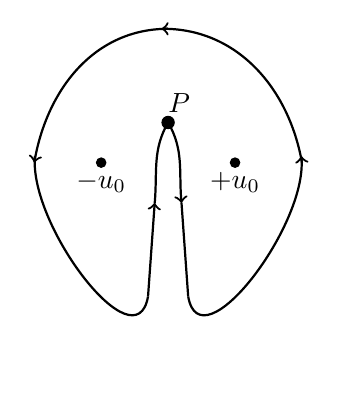
\begin{tikzpicture}[scale=1.7]
        \draw [<-,thick] (0,0) to [out=80,in=180] (1,1);
        \draw [<-,thick] (0.95,1) to [out=0,in=100] (2,0);
        \draw [thick] (0.005,0.05) to [in=-100, out=-95] (0.85,-1);
        \draw[->, thick] (1.15,-1) to [in=-85,out=-80] (1.995,0.05);
        \draw[->,thick] (0.85,-1) to (0.9,-0.3);
        \draw[thick] (0.9,-0.302) to [in=-120,out=85](1,0.3);
        \draw[->, thick] (1,0.3) to [in=95,out=-60](1.1,-0.302);
        \draw [thick] (1.1,-0.3) to (1.15,-1);
        \filldraw(1,0.3) circle (1.3 pt) node[right=4pt,above] {$P$};
        \filldraw (0.5,0) circle (1 pt) node[below] {$-u_{0}$};
        \filldraw (1.5,0) circle (1 pt) node[below] {$+u_{0}$};
    \end{tikzpicture}
    \vspace{3 mm}
    \caption{复平面大$\,\lvert u\rvert\,$值处的逆时针围道形变到一个从基点$\,P\,$出发, 逆时针绕行$\,-u_{0}\,$处的奇点一圈回到$\,P$, 再以逆时针绕行$\,+u_{0}\,$处的奇点一圈回到$\,P\,$的围道.}%
    \label{fig:29.1}%
  \end{figure}
  

我们来考虑只有两个奇点的可能性. (这被证明是参考文献[10]中\,Seiberg\,和\,Witten\,的第二篇文章所考虑的情况.) 在$\,a_{A}\to\mi a_{A}\,$的$\,\mathds{Z}_{8}\,$-对称性下, 我们有$\,u\to-u$, 所以奇点所在的$\,u\,$值必须是成对的, 记为$\,u_{0}\,$和$\,-u_{0}$. 从$\,u\,$空间中的一个非奇异基点$\,P\,$出发, 
然后以逆时针方向绕行$\,\pm u_{0}\,$处的两个奇点一圈回到$\,P$, 这将会产生一个等价的理论. 因此它必须采取对偶变换的形式, 一般会依赖于$\,P$, 
在这个变换中, 矢量$\,(a,a_{D})\,$要乘以一个$\,SL(2,\mathds{Z})\,$单值矩阵$\,M_{\pm}$, 就像方程(\ref{29.5.43})中那样. 
在固定的大$\,u\,$值处的逆时针围道可以形变成一个从$\,P\,$出发, 逆时针绕行$\,-u_{0}\,$一圈回到$\,P$, 再以逆时针绕行$\,+u_{0}\,$一圈回到$\,P$. 
(参看图\ref{fig:29.1}.) 由于这个形变不会改变积分, 单值矩阵在{\kai{这个顺序}}(从右往左读)下的乘积必须等于方程(\ref{29.5.56})中的矩阵:
\begin{equation}
    M_{+}M_{-} = M_{\infty} \equiv
    \begin{pmatrix}
    -1 & 0 \\ 2 & -1
    \end{pmatrix} \:. \label{29.5.57}
\end{equation}
当$\,a\,$和$\,a_{D}\,$所在的值使得某个粒子的质量为零时, 奇点会出现. 例如, 在$\,h(a)\,$的微扰论公式(\ref{29.5.52}) 中, $a=0\,$处有奇点是因为, 当$\,a\,$取这个值时, 基本带电荷粒子在微扰论中变成无质量的. 我们已经排除了只在$\,a=0\,$处有一个奇点的可能性, 
所以$\,\pm u_{0}\,$处的奇点必然来自于其它一些粒子的质量归零.

Seiberg--Witten\,计算的最显著部分是他们意识到这些粒子是底层$\,SU(2)\,$超对理论中发现的非基本磁单极子或双荷子. 
23.3\,节所做的那类半经典计算表明稳定的磁单极子和双核子有磁荷量子数$\,m=\pm 1\,$而电荷量子数$\,n\,$则是任意整数, 
并且这些粒子属于极多重态, 每个极多重态由一对\,Majorana\,旋量和一对复标量构成. 它们是``短''多重态, 质量由\,BPS\,值给出, 
而根据方程(\ref{27.9.24}) 和(\ref{29.5.47}), 这个值是
\begin{equation}
    M=\lvert Z_{12} \rvert/2 =\sqrt{2}\Bigl\lvert Na + h(a) \Bigr\rvert \:, \label{29.5.58}
\end{equation}
其中$\,N\equiv \pm n$. 计算在这个质量趋于零时发生了什么的最简单方法是考虑我们更加熟悉的问题: 当普通带电粒子的极多重态的质量趋于零时发生了什么, 然后使用对偶性转换会一个轻单极子的情况. $U(1)\,$规范耦合的$\,\beta\,$函数在这里由$\,C_{1}=0,$ $C_{2}^{f}=C_{2}^{s}=2\,$的方程(\ref{27.9.45})给出, 所以
\[
\beta(e)= +\frac{e^{3}}{8\uppi^{2}} \:.
\]
那么重整化群方程的解就是
\[
e^{-2}(a) = -\frac{1}{4\uppi^{2}}\ln \biggl(\frac{a}{\text{常数}}\biggr) \:.
\]
正如我们在推导方程(\ref{29.5.52})时所看到的, 这给出
\[
h^{\prime}(a) = 4\uppi\mi\,e^{-2}(a) = -\frac{\mi}{\uppi} \ln \biggl(\frac{a}{\text{常数}}\biggr) \:.
\]
因为这给出的$\,e^{2}(a)\,$在$\,a\to 0\,$时是一个小的正值, 所以, 如果理论确实包含普通带电粒子的极多重态且极多重态的质量在这个极限下为零, 那么这个公式是{\kai{可信}}的. 事实也的确如此, 我们假定存在质量趋于零的单极子或双荷子的极多重态, 为了处理这个情况, 我们可以使用将$\,a\,$变至$\,N(a)+h(a)\,$的对偶变换(\ref{29.5.43})
\begin{equation}
    \begin{pmatrix}
    a \\ h(a)
    \end{pmatrix} \to
    \begin{pmatrix}
    \hat{a} \\ \hat{h}(\hat{a})
    \end{pmatrix} =
    \begin{pmatrix}
    N & +1 \\ -1 & 0
    \end{pmatrix}
    \begin{pmatrix}
    a \\ h(a)
    \end{pmatrix} \:. \label{29.5.59}
\end{equation}
我们由此得出, 当$\,u\,$趋于使得$\,\hat{a}=Na+h(a)\to0\,$的点$\,u_{0}$, 我们有
\begin{equation}
    \frac{\dif \hat{h}(\hat{a})}{\dif \hat{a}} \to -\frac{\mi}{\uppi}
     \ln \biggl(\frac{\hat{a}}{\text{常数}}\biggr) \:, \label{29.5.60}
\end{equation}
或者, 换另一种形式,
\begin{equation}
    \frac{\dif a}{\dif (h(a)+Na)} \to +\frac{\mi}{\uppi} \ln \biggl(\frac{h(a)+Na}{\text{常数}}\biggr) \:. \label{29.5.61}
\end{equation}
解是
\begin{equation}
    a(u) = a_{0}+\frac{\mi}{\uppi}\Bigl(h(a)+Na(u)\Bigr)\ln\biggl(\frac{h(u)+Na(u)}{\Lambda_{0}}\biggr)\:, \label{29.5.62}
\end{equation}
其中$\,a_{0}\,$和$\,\Lambda_{0}\,$是积分常数. 我们还假定了在$u\to u_{0}\,$时, $h+Na\to0$, 所以我们可以把领头项写成
\begin{equation}
    h(u)+Na(u)\to c_{0}(u-u_{0}) \:. \label{29.5.63}
\end{equation}
因此方程(\ref{29.5.62})有领头项
\begin{equation}
    a(u)\to a_{0} +\frac{\mi\,c_{0}}{\uppi}(u-u_{0}) \ln\biggl(\frac{c_{0}(u-u_{0})}{\Lambda_{0}}\biggr) \:.
    \label{29.5.64}
\end{equation}

当我们让$\,u\,$围绕$\,u_{0}\,$逆时针绕行一圈时, $h(a)+Na\,$没有变化, 但$\,a\,$会被偏移$\,-2(h(a)+Na)$, 
所以这个奇点的单值矩阵是
\begin{equation}
    M_{+} = \begin{pmatrix}
    1-2N & -2 \\ 2N^{2} & 1+2N
    \end{pmatrix} \:. \label{29.5.65}
\end{equation}

同理, 如果$\,-u_{0}\,$处的奇点所对应的质量为零的单极子和双荷子有磁荷量子数$\,\pm'1\,$(撇号是为了与$\,u_{0}\,$的符号相区分)和电荷量子数$\,n'$, 那么在这个奇点处$\,h(u)\to N'a(u)\to 0$, 且
\begin{equation}
    a \to a_{0}^{\prime} + \frac{\mi}{\uppi}\Bigl(h(u) + N^{\prime}a(u)\Bigr)
    \ln\biggl(\frac{h(u)+N^{\prime}a(u)}{\Lambda_{0}^{\prime}} \biggr) \:, \label{29.5.66}
\end{equation}
其中$\,N'\equiv \pm'n'\,$而$\,a_{0}'\,$和$\,\Lambda_{0}'$是新的积分常数. 领头项是
\begin{equation}
    h(u) + N^{\prime}a(u) \to c_{0}^{\prime}(u+u_{0}) \:, \label{29.5.67}
\end{equation}
\begin{equation}
    a \to a_{0}^{\prime}+\frac{\mi\, c_{0}^{\prime}}{\uppi} (u+u_{0})
    \ln\biggl(\frac{c_{0}^{\prime}(u+u_{0})}{\Lambda_{0}^{\prime}}\biggr) \label{29.5.68}
\end{equation}
这个奇点的单值矩阵是
\begin{equation}
    M_{-}=\begin{pmatrix}
    1-2N^{\prime} & -2 \\ 2N^{\prime2} & 1+2N^{\prime}
    \end{pmatrix} \:. \label{29.5.69}
\end{equation}
这样直接就能看到, 当且仅当
\begin{equation}
    N^{\prime} = N-1 \:, \label{29.5.70}
\end{equation}
这些矩阵上的条件(\ref{29.5.57})才是满足的. 我们对$\,N\,$取什么值并不会有影响, 这是因为通过绕着无穷远处的圈$\,M\,$次, 我们可以将其偏移偶数$\,2M$, 而通过反射$\,u\to-u$, 我们可以将其偏移\,1. Seiberg 和\,Witten\,选择取$\,N=0$, 这使得$\,N'=-1$. 那么在$\,u\to u_{0}\,$时, 
\begin{equation}
    h(u)\to c_{0}(u-u_{0}) \:, \label{29.5.71}
\end{equation}
\begin{equation}
    a(u)\to a_{0}+\frac{\mi\,c_{0}}{\uppi}(u-u_{0})\ln\biggl(\frac{u-u_{0}}{\Lambda_{0}}\biggr) \:, \label{29.5.72}
\end{equation}
以及在$\,u\to-u_{0}\,$时
\begin{equation}
    h(u)-a(u)\to c_{0}^{\prime}(u+u_{0}) \:, \label{29.5.73}
\end{equation}
\begin{equation}
    a(u) \to a_{0}^{\prime} + \frac{\mi\, c_{0}^{\prime}}{\uppi}(u+u_{0})
    \ln\biggl(\frac{u+u_{0}}{\Lambda_{0}^{\prime}}\biggr) \:. \label{29.5.74}
\end{equation}

我们现在附加未破缺的$\,\mathds{Z}_{8}\,$-对称性条件(\ref{29.5.54}). 我们可以通过将$\,a(u)\,$写成$\,-\mi a(-u)\,$并使用方程(\ref{29.5.72})来计算它在$\,u\to-u_{0}\,$时的值. 那么, 在$\,u\to -u_{0}\,$时
\begin{equation}
    a(u) \to -\mi a_{0} + \frac{c_{0}}{\uppi}\ln\biggl(\frac{-c_{0}(u+u_{0})}{\Lambda_{0}}\biggr)\:. \label{29.5.75}
\end{equation}
与方程(\ref{29.5.74})相比较, 我们看到$\,c_{0}'=\mi c_{0}$, 所以在$\,u\to -u_{0}\,$时, 方程变成
\begin{equation}
    h(u)-a(u) \to \mi\,c_{0}\,(u+u_{0}) \:. \label{29.5.76}
\end{equation}

场$\,a\,$在定义包含了一个规范耦合因子$\,e$, 通过合适选择计算$\,e\,$的重整化点, $e\,$可以被赋予任何值. 
Seiberg\,和\,Witten\,选择定义$\,a\,$和$\,u\,$(保持$\,u=a^{2}/2\,$在无穷远处)的标度使得$\,u_{0}=1$; 
即奇点处在$\,u=\pm 1\,$处. 在这个约定下, 他们获得了解(定义解的复平面有$\,-1\,$到$\,+1\,$的割线)
\begin{equation}
    a_{\text{SW}}(u) =\frac{\sqrt{2}}{\uppi}\int_{-1}^{1}\dif x\: \sqrt{\frac{u-x}{1-x^{2}}} \:, \label{29.5.77}
\end{equation}
\begin{equation}
    h_{\text{SW}}(u) =\frac{\mi\,\sqrt{2}}{\uppi}\int_{1}^{u}\dif x\: \sqrt{\frac{u-x}{1-x^{2}}} \:. \label{29.5.78}
\end{equation}
最初用来获得这些结果的数学方法超出了本书的范围, 但幸运的是, 检验它们正确并不困难.

首先, 作为正确的解, 我们可以验证$\,a_{\text{SW}}(u)\,$和$\,h_{\text{SW}}(u)\,$在$\,u=\pm 1\,$处的奇点与(\ref{29.5.71}), 
(\ref{29.5.72}), (\ref{29.5.75})和(\ref{29.5.76})形式相同. 当$\,u\to 1\,$时, 方程(\ref{29.5.77})给出 
\begin{align}
    a_{\text{SW}}(u) &\to \frac{\sqrt{2}}{\uppi} \int_{-1}^{1}\frac{\dif x}{\sqrt{x+1}}
    +\frac{u-1}{2\uppi}\int_{-1}^{1}\frac{\dif x}{\sqrt{(1-x)(u-x)}} \nonumber \\
    &= \frac{4}{\sqrt{\uppi}} + \frac{u-1}{2\uppi}
    \ln\Biggl(\frac{u-1}{3+u-2\sqrt{2}\sqrt{1+u}}\Biggr) \nonumber \\
    &\to \frac{4}{\sqrt{\uppi}} - \frac{u-1}{2\uppi} \ln\Bigl(4(u-1)\Bigr) \:. \label{29.5.79}
\end{align}
另外, 方程(\ref{29.5.78})给出
\begin{equation}
    h_{\text{SW}}(u) \to \frac{\mi}{\uppi}\int_{1}^{u}\dif x\:\sqrt{\frac{u-x}{x-1}}
    = \frac{\mi(u-1)}{2} \:. \label{29.5.80}
\end{equation}
方程(\ref{29.5.79})和(\ref{29.5.80})与我们之前的结果(\ref{29.5.71})和(\ref{29.5.72})在$\,c_{0}=\mi\,$和$\,a_{0}=4/\sqrt{\uppi}\,$给出的值一致. 方程(\ref{29.5.77})满足$\,\mathds{Z}_{8}\,$反射性质(\ref{29.5.54}), 所以$\,a_{\text{SW}}(u)\,$在$\,u\to -1\,$时的行为自动是(\ref{29.5.75}), 并且(要注意从$\,u=-1\,$到$\,u=+1\,$的割线对平方根符号的影响)由此可以直接从方程(\ref{29.5.77})和 (\ref{29.5.78})得出$\,h_{\text{SW}}(u)-a_{\text{SW}}(u)\,$在$\,u\,$接近$\,-1\,$时正比于$\,u+1$. 


现在, 由于$\,a_{\text{SW}}\,$和$\,h_{\text{SW}}(u)\,$在$\,u\to\pm 1\,$处的奇点结构与$\,a(u)\,$和$\,h(u)\,$相同, 
它们有相同的单值性($N=0\,$和$\,N'=-1\,$的方程(\ref{29.5.59})和(\ref{29.5.69})): 当$\,u\,$绕点$\,+1\,$一圈, 我们有
\begin{equation}
    \begin{pmatrix}
    a_{\text{SW}} \\ h_{\text{SW}}
    \end{pmatrix} \to
    \begin{pmatrix}
     0 & +1 \\ -1 & 0
    \end{pmatrix}
    \begin{pmatrix}
    a_{\text{SW}} \\ h_{\text{SW}}
    \end{pmatrix} \:, \label{29.5.81}
\end{equation}
而当$\,u\,$绕点$\,-1\,$一圈,
\begin{equation}
    \begin{pmatrix}
    a_{\text{SW}} \\ h_{\text{SW}}
    \end{pmatrix} \to
    \begin{pmatrix}
    3 & -2 \\ 2 & -1
    \end{pmatrix}
    \begin{pmatrix}
    a_{\text{SW}} \\ h_{\text{SW}}
    \end{pmatrix} \:. \label{29.5.82}
\end{equation}


我们现在来考虑
\begin{equation}
    f(u)\equiv a(u) h_{\text{SW}}(u) - a_{\text{SW}}(u)h(u) \:. \label{29.5.83}
\end{equation}
这是一个$\,SL(2,\mathds{Z})\,$不变量, 所以它的单值性是平庸的: 当$\,u\,$绕着$\,+1\,$或$\,-1\,$一圈后, 它的值不变. 
$a(u)$, $h(u)$, $a_{\text{SW}}(u)\,$或$\,h_{\text{SW}}(u)\,$在有限处的奇点只能是在$\,\pm 1\,$处的对数奇点, 
但由于$\,f(u)\,$的单值性是平庸的, 它没有这些奇点, 因此它在所有的有限点处都是解析的.

为了计算全纯函数$\,f(u)$, 我们首先要验证函数$\,a_{\text{SW}}(u)\,$和$\,h_{\text{SW}}(u)\,$的渐进行为中的领头项分别
与$\,a(u)\,$和$\,h(u)\,$相同. 在$\,u\to\infty\,$时, 方程(\ref{29.5.77})给出
\begin{equation}
    a_{\text{SW}}(u)\to \frac{\sqrt{2u}}{\uppi} \int_{-1}^{1}\frac{\dif x}{\sqrt{1-x^{2}}} =\sqrt{2u} \:, \label{29.5.84}
\end{equation}
而方程(\ref{29.5.78})给出
\begin{equation}
    h_{\text{SW}}(u)\to \frac{\mi\sqrt{2u}}{\uppi} \int_{1}^{u}\frac{\dif x}{\sqrt{x^{2}-1}}
    \to  \frac{\mi\sqrt{2u}}{\uppi} \sqrt{u}\ln u  \:, \label{29.5.85}
\end{equation}
这与$\,a(u)\,$和$\,h(u)\,$的领头行为(\ref{29.5.55})相同.

这本身只证明了在$\,u\to\infty\,$时$\,f(u)/u\ln u\to 0$. 但注意到, $a(u)\,$的反射对称性(\ref{29.5.54})以及$\,a_{\text{SW}}(u)\,$的类似对称性告诉我们两个函数中的次领头项是$\,\sqrt{u}/u^{2}\,$阶的. 另外, $h(u)\,$和$\,h_{\text{SW}}(u)\,$中的次领头项是$\,\sqrt{u}\,$阶的. 由此得出我们可以通过令$\,a(u)=a_{\text{SW}}(u)=\sqrt{2u}\,$来计算$\,f(u)\,$渐进行为中的领头项, 
这使得在$\,u\to\infty\,$时$\,f(u)=O(u)$. 由于$\,f(u)\,$是全纯函数, 这意味着$\,f(u)\,$关于$\,u\,$是线性的. 
然而, $f(u)\,$在$\,u=+1\,$处为零, $h(u)\,$和$\,h_{\text{SW}}(u)\,$在这里是$\,O(u-1)$, 而$\,f(u)\,$也在$\,u=-1\,$处为零, 
$a(u)-h(u)\,$和$\,a_{\text{SW}}(u)-h_{\text{SW}}(u)\,$在这里则是$\,O(u-1)$, 所以$\,f(u)\,$必须处处为零. 我们由此得出
\begin{equation}
    \frac{a_{\text{SW}}(u)}{a(u)} = \frac{h_{\text{SW}}(u)}{h(u)} \equiv g(u) \:. \label{29.5.86}
\end{equation}
现在我们必须考虑函数$\,g(u)\,$的性质. 因为$\,h_{\text{SW}}(u)\,$和$\,h(u)\,$在$\,u=-1\,$以外的所有有限点处都是解析的, 
而$\,a(u)-h(u)\,$和$\,a_{\text{SW}}(u)-h_{\text{SW}}(u)\,$在$\,u=+1\,$以外的所有有限点处都是解析的, 
由此得出$\,g(u)\,$(也可以写为$[a_{\text{SW}}(u)-h_{\text{SW}}(u)]/[a(u)-h(u)]$)处处解析. ($a(u)\,$或$\,h(u)\,$在$\,u\neq\pm 1\,$是没有零点, 更何况二者的共同零点, 这是因为, 在$\,a(u)\,$或$\,h(u)\,$的零点处, 带电粒子或单极子的质量为零, 而我们已经假定对任何$\,u\neq \pm 1\,$都不是这样的情况.) 另外, 函数$\,a_{\text{SW}}(u)\,$和$\,h_{\text{SW}}(u)\,$在$\,u\to\infty\,$时的渐进行为中的领头项分别与$\,a(u)\,$和$\,h(u)\,$的相同, 这个性质意味着在$\,u\to\infty\,$时$\,g(u)\to 1$. 由此得出全纯函数$\,g(u)\,$对所有$\,u\,$都必须等于\,1, 因此
\begin{equation}
    a(u)=a_{\text{SW}}(u) \:, \qquad h(u)=h_{\text{SW}}(u) \:, \label{29.5.87}
\end{equation}
这正是所要证明的.



\section*{习题}
\noindent 1. 对于第\,\ref{cha:26}\,章习题\,4\,中的模型, 它在$\,a\neq 0\,$时的\,Witten\,指标是多少? $a=0\,$是多少? 
在$\,a=0\,$时, 这个模型中的超对称性是否会被高阶效应破缺? 试解释. \\

\noindent 2. 考虑这样的可重整超对称理论, 它有$\,SO(N_{c})\,$规范对称性以及$\,N_{f}\,$个处在$\,N\,$-矢量表示下的左手征标量超场$\,\Phi_{n}$. 当裸超势为零时, 你能对非微扰威尔逊型拉格朗日密度的非微扰结构说些什么? 如果有一个裸超势$\,\sum_{n}\Phi_{n}\Phi_{n}\,$又将如何? \\

\noindent 3. 在拉格朗日密度是(\ref{29.5.22})的理论中, 旋量场强超场$\,W_{\alpha}\,$的分量场与其对偶$\,\tilde{W}_{\alpha}\,$的分量场之间有什么关系? \\


%++++++++++++++++++参考文献+++++++++
\renewcommand{\sectionmark}[1]{\markright{ #1}{}}
\renewcommand{\bibname}{参考文献}

\begin{thebibliography}{99}
    \bibitem{1} E. Witten, {\textit{Nucl. Phys.}} {\bf{B185}}, 513 (1981), 这篇文章重印于{\textit{Supersymmetry}}, S. Ferrara\,编辑(North Holland/World Scientific, Amsterdam/Singapore, 1987).
    \bibitem[1a]{1a} J. Hughes and J. Polchinski, {\textit{Nucl. Phys.}} {\bf{B278}}, 147 (1986); J. Hughes, J. Liu, and J. Polchinski, {\textit{Phys. Lett.}} {\bf{B180}}, 370 (1986); J. Bagger and A. Galperin, {\textit{Phys. Lett.}} {\bf{B336}}, 25 (1994); {\textit{Phys. Rev.}} {\bf{D55}}, 1091 (1997); {\textit{Phys. Lett.}} {\bf{412}}, 296 (1997); L. Antoniadis, H. Partouche, and T. R. Taylor, {\textit{Phys. Lett.}} {\bf{B372}}, 83 (1996); S. Ferrara, L. Girardello, and M. Porrati, {\textit{Phys. Lett.}} {\bf{B376}}, 275 (1996).
    \bibitem{2} E. Witten, {\textit{Nucl. Phys.}} {\bf{B202}}, 253 (1982). 这篇文章重印于{\textit{Supersymmetry}}, 参考文献[1].
    \bibitem{3} A. C. Davis, M. Dine, and N. Seiberg, {\textit{Phys. Lett}}. {\bf{125B}}, 487 (1983); I. Affleck, M. Dine, and N. Seiberg, {\textit{Phys. Rev. Lett.}} {\bf{51}}, 1026 (1983); {\textit{Phys. Lett.}} {\bf{137B}}, 187 (1984), 重印于{\textit{Supersymmetry}}, 参考文献[1]; {\textit{Nucl. Phys.}} {\bf{B241}}, 493 (1984); {\textit{Nucl. Phys.}} {\bf{B52}}, 1677 (1984); {\textit{Phys. Lett.}} {\bf{140B}}, 59 (1984).
    \bibitem{4} N. Seiberg, {\textit{Phys. Lett.}} {\bf{B318}}, 469 (1993).
    \bibitem{5} V. A. Novikov, M. A. Shifman, A. I. Vainshtein, and V. I. Zakharov, {\textit{Nucl. Phys.}} {\bf{B229}}, 381 (1983); {\textit{Nucl. Phys.}} {\bf{B260}}, 157 (1985); G. C. Rossi and G. Veneziano, {\textit{Phys. Lett.}} {\bf{138B}}, 195 (1984), 重印于{\textit{Supersymmetry}}, %
        参考文献[1]. 综述可参看\,M. A. Shifman and A. I. Vainshtein, hep-th/9902018, 待发表.
    \bibitem{6} E. Witten, {\textit{J. High Energy Phys.}} {\bf{9802}}, 006 (1998).
    \bibitem{7} V. G. Kac and A. V. Smilga, hep-th/9902029, 待发表.
    \bibitem{8} I. Affleck, M. Dine, and N. Seiberg, {\textit{Nucl. Phys.}} {\bf{B256}}, 557 (1985).
    \bibitem{9} N. Seiberg, {\textit{Phys. Rev.}} {\bf{D49}}, 6857 (1994).
    \bibitem{10} N. Seiberg and E. Witten, {\textit{Nucl. Phys.}} {\bf{B426}}, 19 (1994); {\textit{erratum, Nucl. Phys.}} {\bf{B430}}, 485 (1994). N. Seiberg\,和\,E.Witten\,给出了到有物质极多重态的$\,N=2\,$理论的推广, {\textit{Nucl. Phys.}} {\bf{B431}}, 484 (1994). 综述可以参看: K. Intrilligator and N. Seiberg, {\textit{Nucl. Phys. Proc. Suppl.}} {\bf{45BC}}, 1 (1996); 另发表于\,{\textit{Summer School in High Energy Physics and Cosmology, Trieste, 1995}}, E. Gava\,编辑(World Scientific, Singapore, 1997), 又收录于\,{\textit{QCD and Beyond: Proceedings of the Theoretical Advanced Study Institute in Elementary Particle Physics, Boulder Colorado, 1995}}, D. E. Soper\,编辑(World Scientific, Singapore, 1996).
    \bibitem{11} E. Witten, {\textit{Phys. Lett.}} {\bf{86B}}, 283 (1979).
    \bibitem{12} N. Seiberg, {\textit{Phys. Lett.}} {\bf{B206}}, 75 (1988).
\end{thebibliography}
